%% 
%% Copyright 2007-2025 Elsevier Ltd
%% 
%% This file is part of the 'Elsarticle Bundle'.
%% ---------------------------------------------
%% 
%% It may be distributed under the conditions of the LaTeX Project Public
%% License, either version 1.3 of this license or (at your option) any
%% later version.  The latest version of this license is in
%%    http://www.latex-project.org/lppl.txt
%% and version 1.3 or later is part of all distributions of LaTeX
%% version 1999/12/01 or later.
%% 
%% The list of all files belonging to the 'Elsarticle Bundle' is
%% given in the file `manifest.txt'.
%% 
%% Template article for Elsevier's document class `elsarticle'
%% with numbered style bibliographic references
%% SP 2008/03/01
%% $Id: elsarticle-template-num.tex 272 2025-01-09 17:36:26Z rishi $
%%
\documentclass[preprint,12pt]{elsarticle}

%% Use the option review to obtain double line spacing
%% \documentclass[authoryear,preprint,review,12pt]{elsarticle}

%% Use the options 1p,twocolumn; 3p; 3p,twocolumn; 5p; or 5p,twocolumn
%% for a journal layout:
%% \documentclass[final,1p,times]{elsarticle}
%% \documentclass[final,1p,times,twocolumn]{elsarticle}
%% \documentclass[final,3p,times]{elsarticle}
%% \documentclass[final,3p,times,twocolumn]{elsarticle}
%% \documentclass[final,5p,times]{elsarticle}
%% \documentclass[final,5p,times,twocolumn]{elsarticle}

%% For including figures, graphicx.sty has been loaded in
%% elsarticle.cls. If you prefer to use the old commands
%% please give \usepackage{epsfig}

%% The amssymb package provides various useful mathematical symbols
\usepackage{amssymb}
% \usepackage[noend]{algpseudocode}
\usepackage[ruled,vlined]{algorithm2e}

%% The amsmath package provides various useful equation environments.
\usepackage{amsmath}
\usepackage[margin=1in]{geometry}


\usepackage{amsmath}
\usepackage{amsfonts}
\usepackage{amssymb}
\usepackage{graphicx}
\usepackage{booktabs} % For professional looking tables
\usepackage{longtable,makecell,tabularx,booktabs} % For tables that might span multiple pages
\usepackage{multirow}

% Add any other packages you commonly use

%% The amsthm package provides extended theorem environments
%% \usepackage{amsthm}

%% The lineno packages adds line numbers. Start line numbering with
%% \begin{linenumbers}, end it with \end{linenumbers}. Or switch it on
%% for the whole article with \linenumbers.
%% \usepackage{lineno}

\journal{Energy and Buildings}

\begin{document}

\begin{frontmatter}

%% Title, authors and addresses

%% use the tnoteref command within \title for footnotes;
%% use the tnotetext command for theassociated footnote;
%% use the fnref command within \author or \affiliation for footnotes;
%% use the fntext command for theassociated footnote;
%% use the corref command within \author for corresponding author footnotes;
%% use the cortext command for theassociated footnote;
%% use the ead command for the email address,
%% and the form \ead[url] for the home page:
%% \title{Title\tnoteref{label1}}
%% \tnotetext[label1]{}
%% \author{Name\corref{cor1}\fnref{label2}}
%% \ead{email address}
%% \ead[url]{home page}
%% \fntext[label2]{}
%% \cortext[cor1]{}
%% \affiliation{organization={},
%%             addressline={},
%%             city={},
%%             postcode={},
%%             state={},
%%             country={}}
%% \fntext[label3]{}

\title{A Co-Simulation Methodology for Integrating Data-Driven Thermal Sensation Models with Building Energy Control}

%% use optional labels to link authors explicitly to addresses:
%% \author[label1,label2]{}
%% \affiliation[label1]{organization={},
%%             addressline={},
%%             city={},
%%             postcode={},
%%             state={},
%%             country={}}
%%
%% \affiliation[label2]{organization={},
%%             addressline={},
%%             city={},
%%             postcode={},
%%             state={},
%%             country={}}

\author[hku]{Hongshan Guo} %% Author name
\author[hku]{Kanxuan He}
\author[nus]{Yue Lei}
% \author{hku}{Yu Chang}
%% Author affiliation
\affiliation[hku]{organization={Department of Architecture, Faculty of Architecture, The University of Hong Kong},%Department and Organization
            % addressline={}, 
            city={Hong Kong SAR},
            % postcode={}, 
            % state={},
            country={China}}

\affiliation[nus]{organization={Department of Built Environment, National University of Singapore},%Department and Organization
            % addressline={}, 
            % city={Hong Kong SAR},
            % postcode={}, 
            % state={},
            country={Singapore}}

%% Abstract
\begin{abstract}
This paper presents a novel co-simulation methodology that directly integrates data-driven thermal sensation models with EnergyPlus building control, addressing the gap between comfort prediction research and practical HVAC implementation. Our framework enables real-time coupling of any comfort predictor—from analytical PMV to deep learning models—with building control while handling actuator saturation and stochastic disturbances. 
We demonstrate the methodology by implementing seven control strategies using models trained on 148,148 occupant votes, including PMV, LightGBM, and a physics-informed neural network-variational autoencoder (PINN-VAE), revealing critical implementation challenges such as actuator saturation in ML-based controllers.
The framework reveals unexpected insights: grid-search optimized PMV achieves 15–18.5\% energy savings comparable to sophisticated ML models while requiring no training data and completing simulations 50x faster. All optimized strategies reduce uncomfortable hours from 25\% to below 3\% while saving energy. Furthermore, incorporating PINN-VAE's physiological predictions improves comfort by 14.85\% with minimal energy impact. These findings, enabled by our co-simulation methodology, demonstrate that control integration quality matters more than model sophistication—challenging assumptions about comfort-based building control and providing essential infrastructure for realistic control strategy evaluation.
\end{abstract}
%%Graphical abstract
\begin{graphicalabstract}
\centering
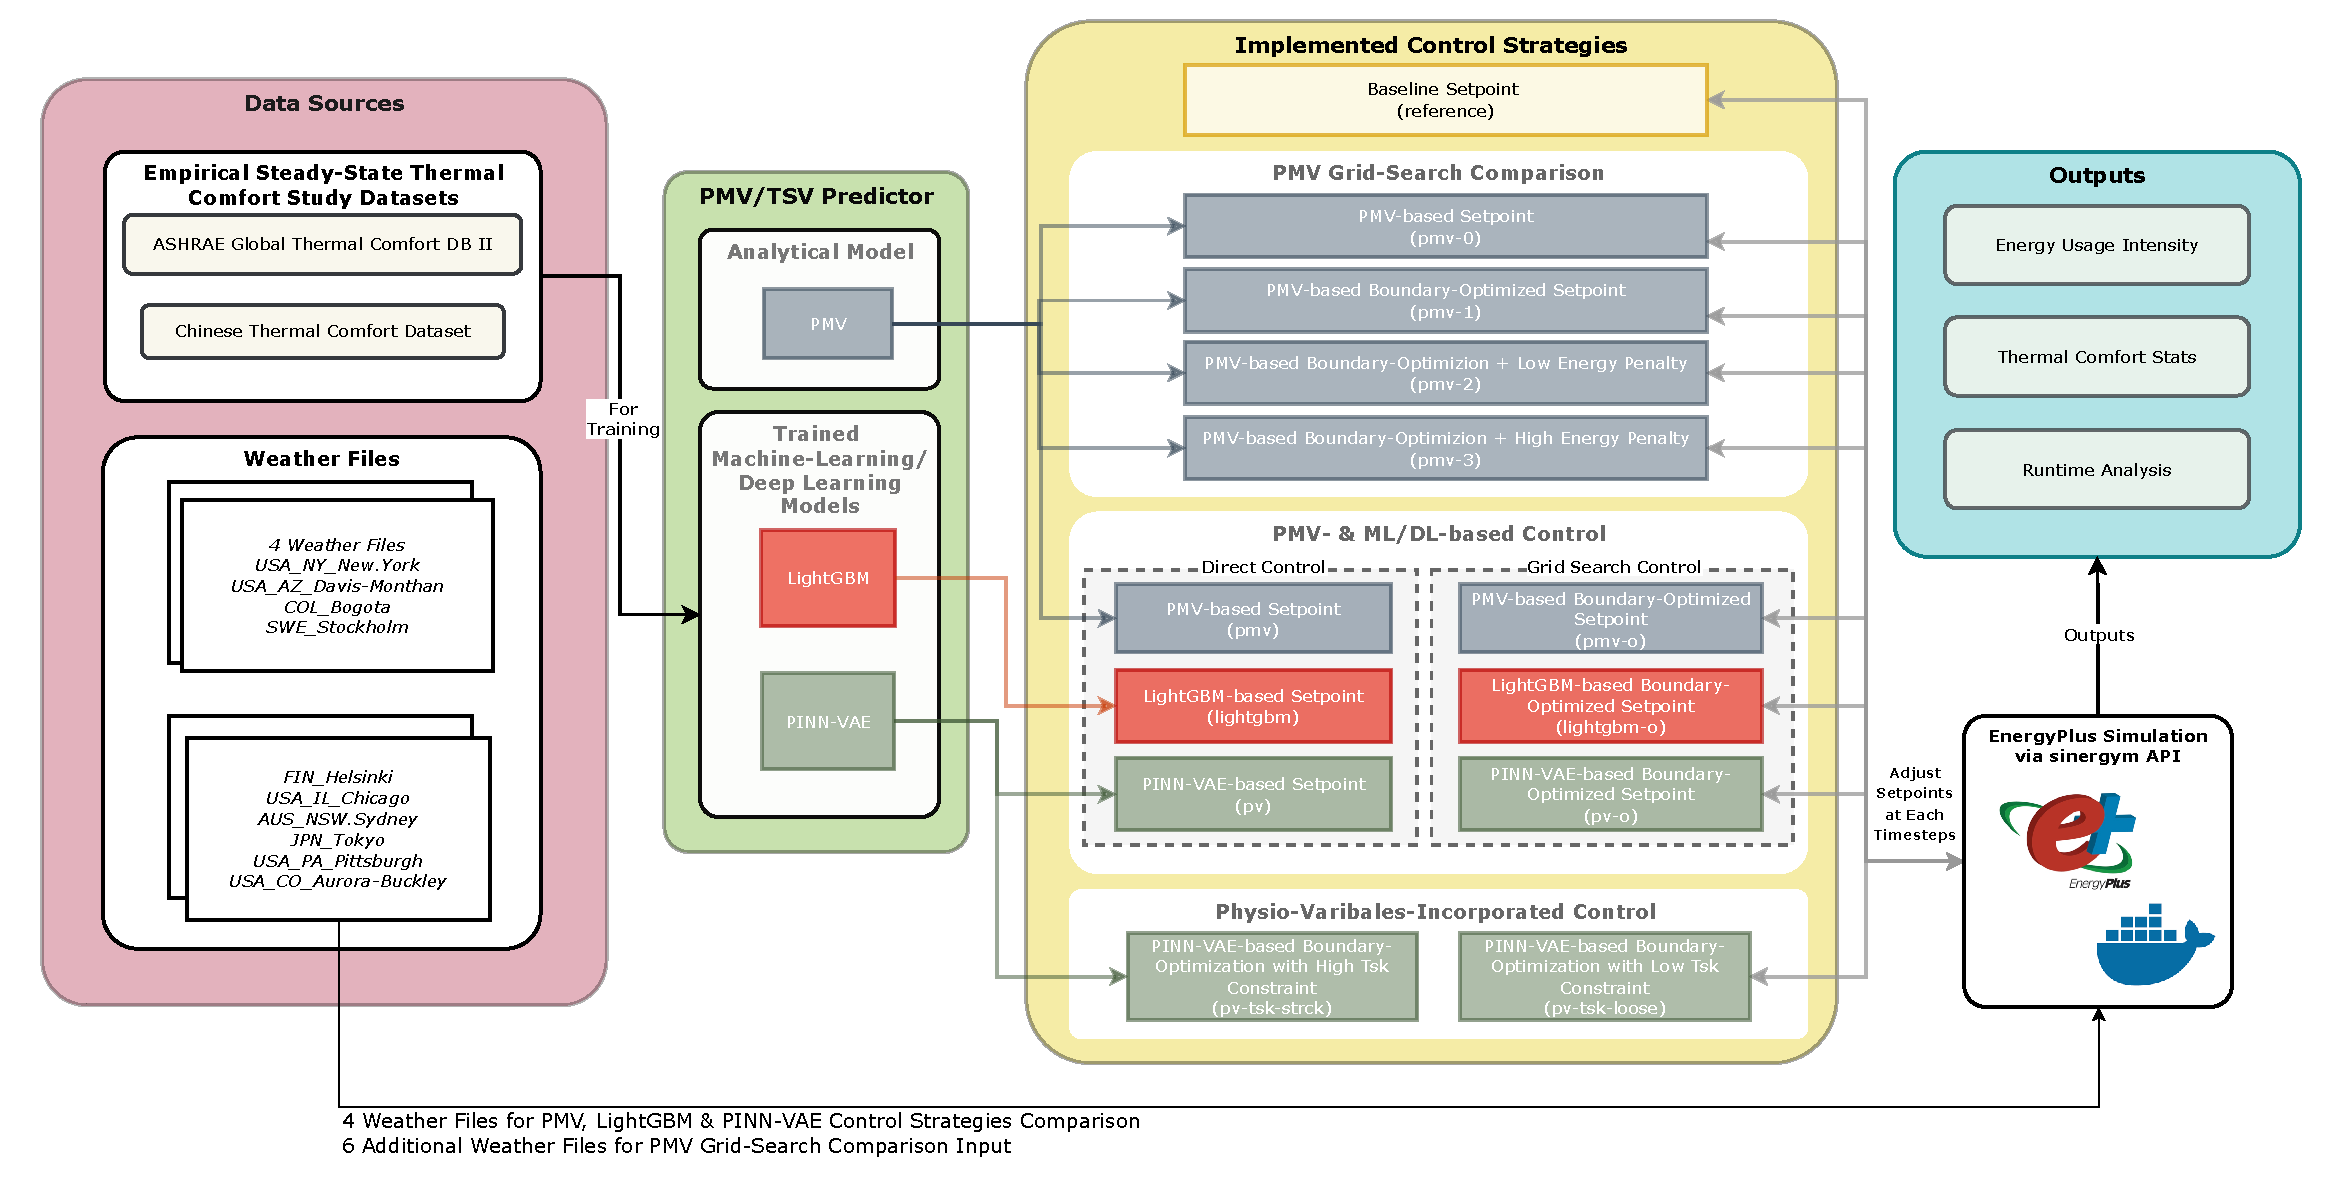
\includegraphics[width=.90\linewidth]{figs/gridworkflow_3.pdf}\\
\\
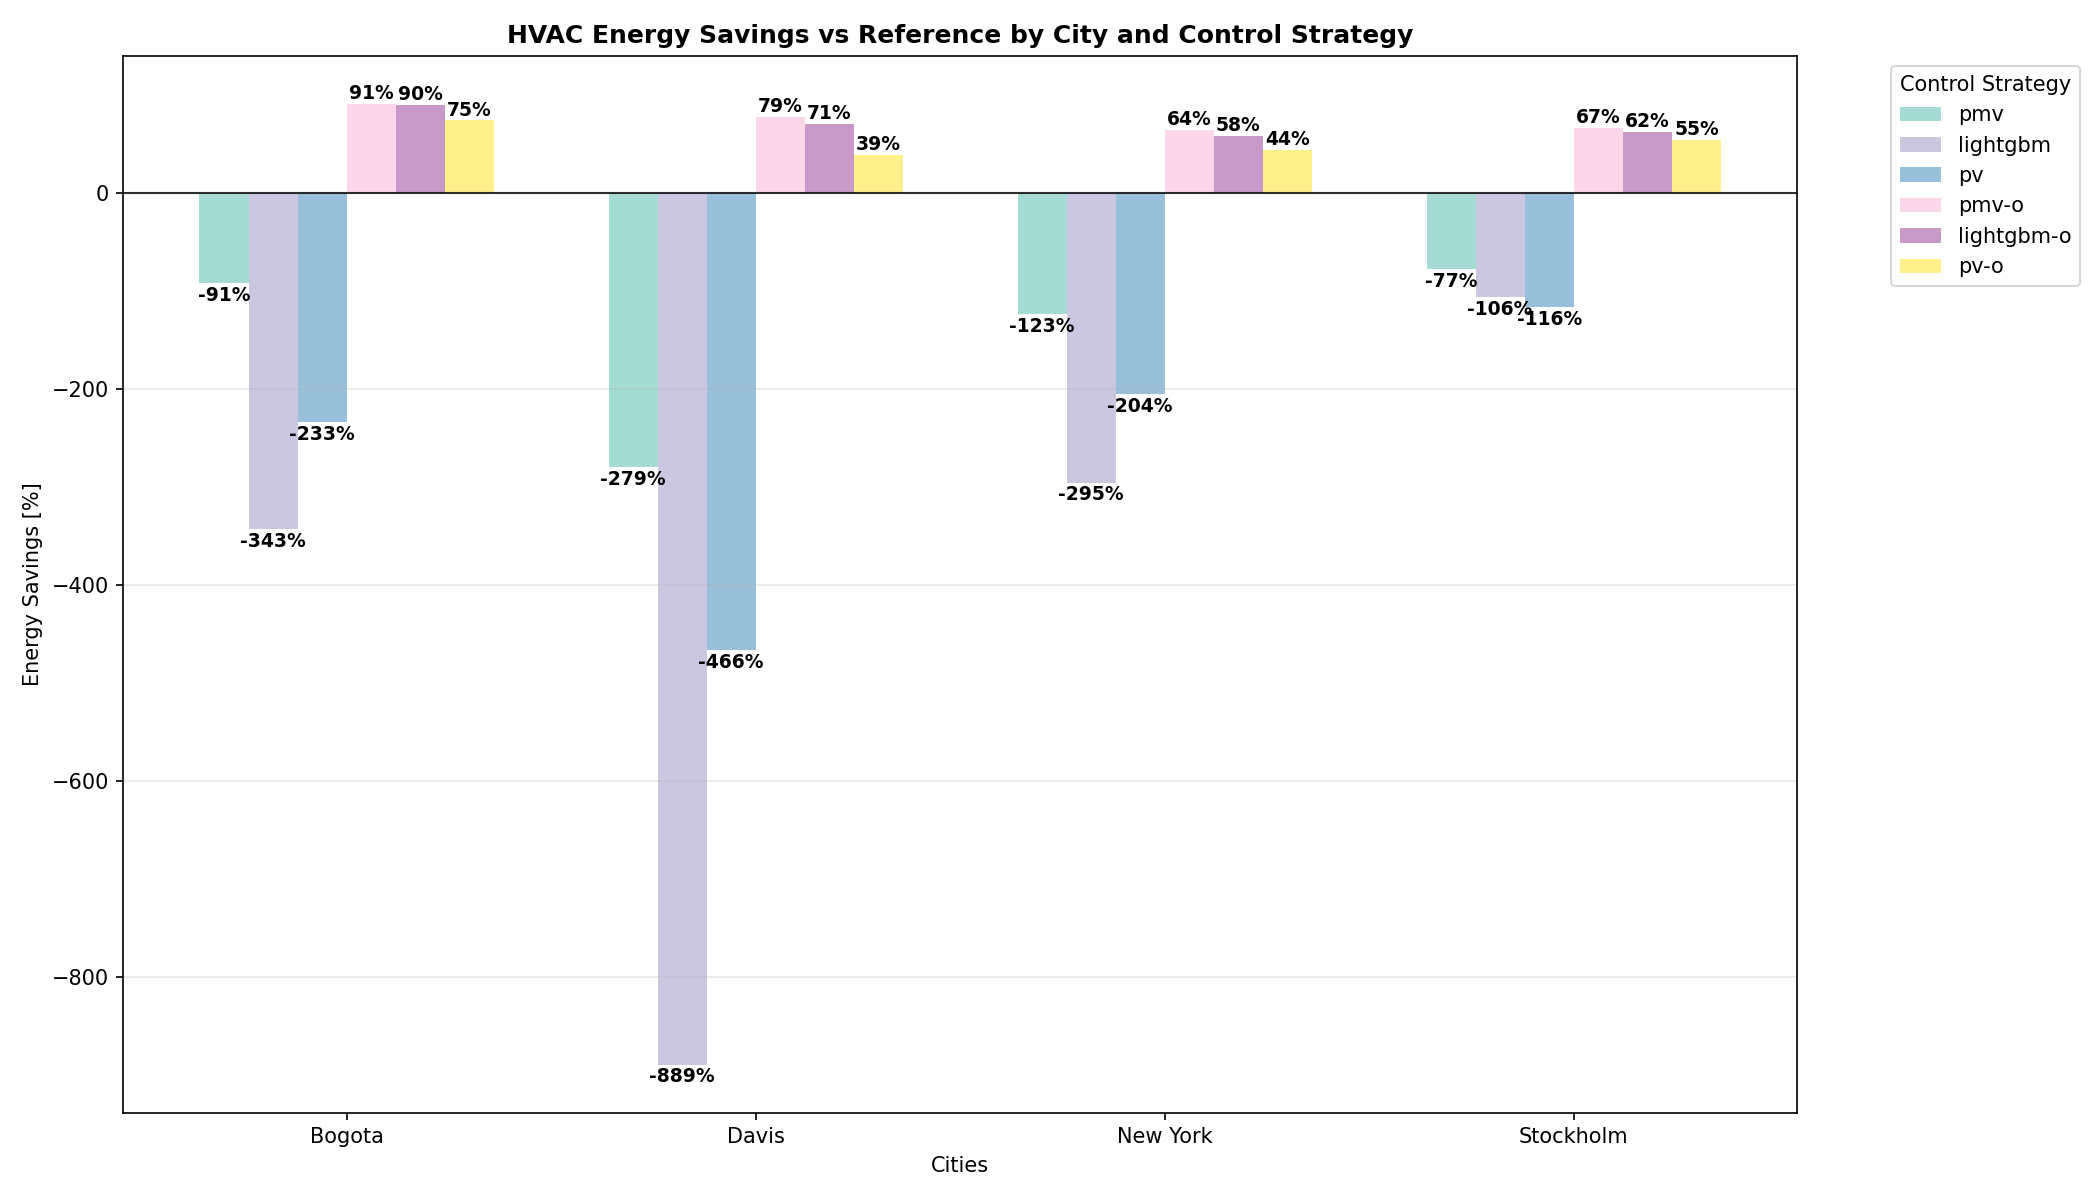
\includegraphics[width=.65\linewidth]{figs/savings_r.png}\\
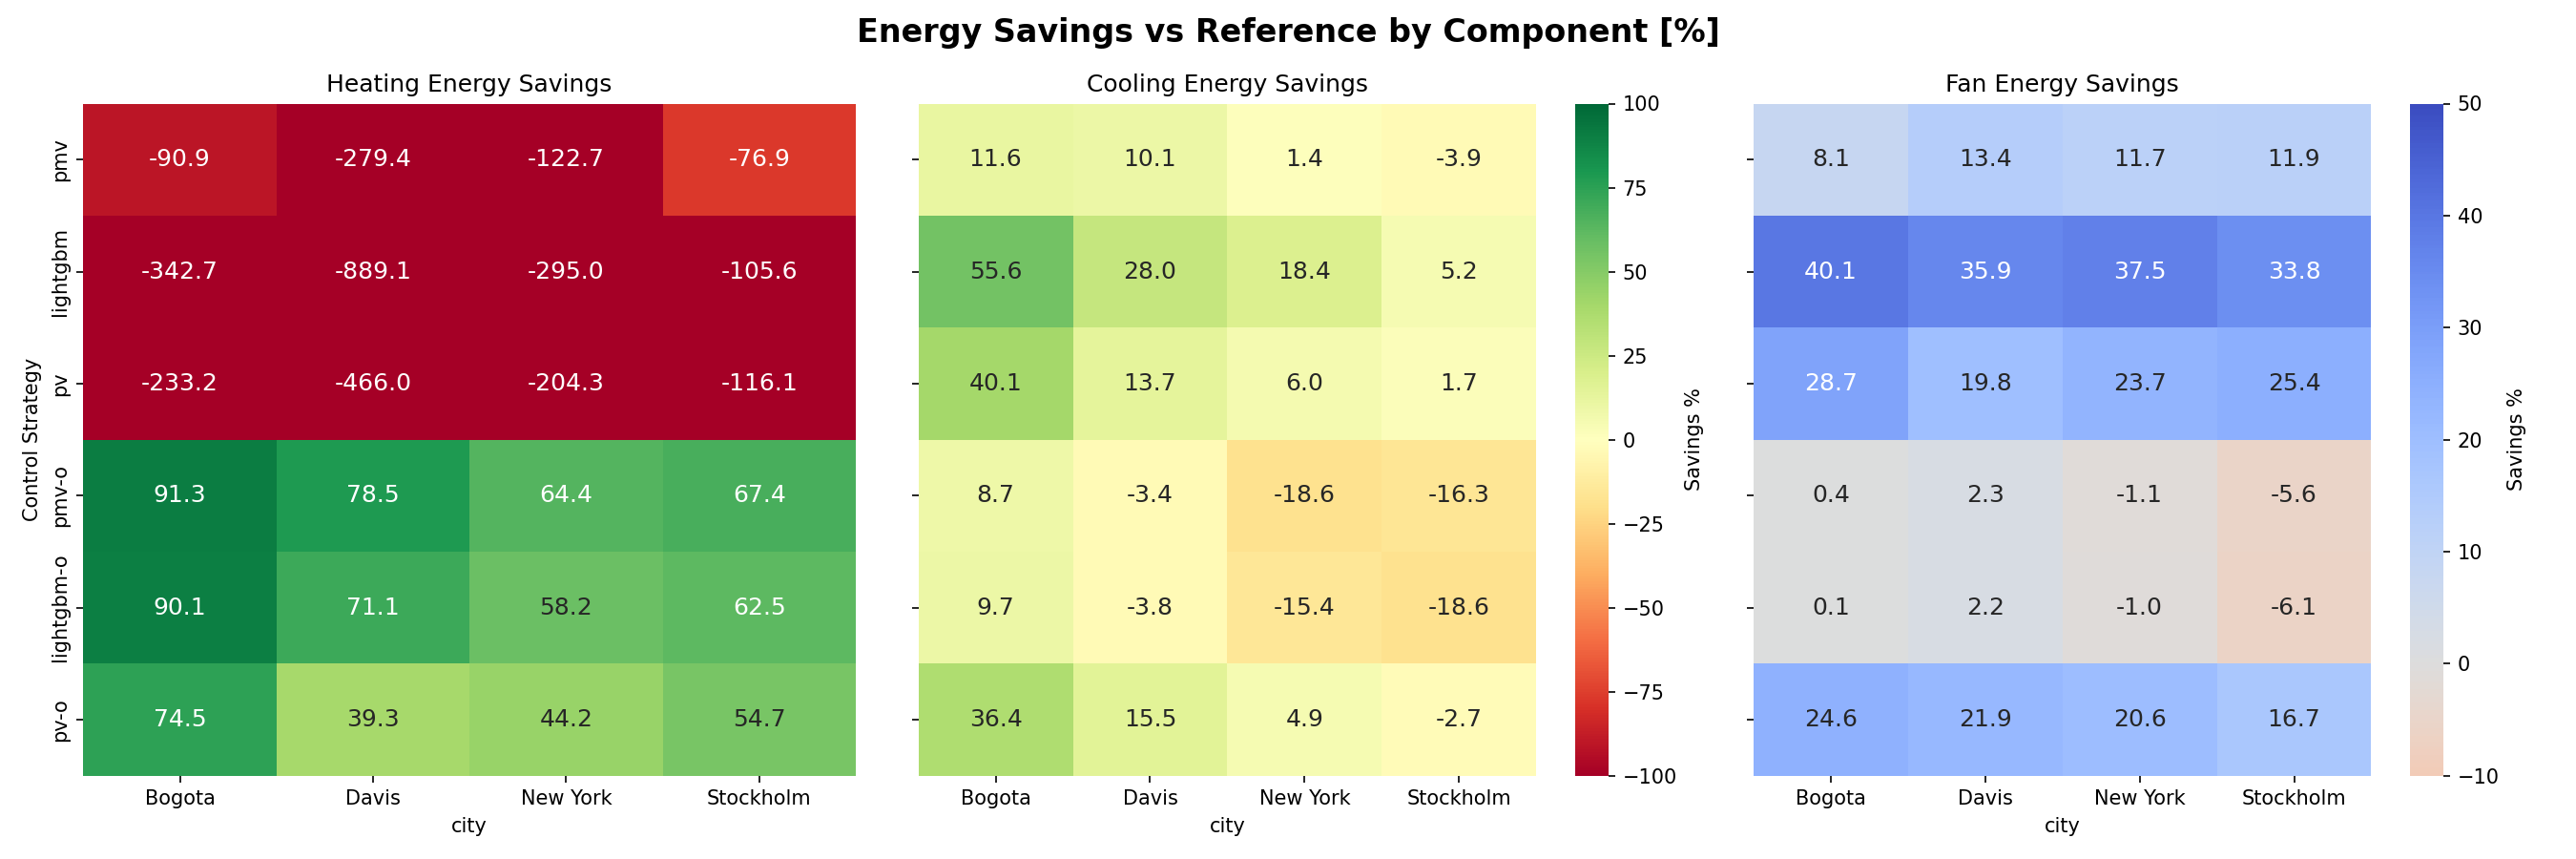
\includegraphics[width=.95\linewidth]{figs/saving_end_pct.png}
%
\includegraphics{grabs}
\end{graphicalabstract}

%%Research highlights
\begin{highlights}
\item Co-simulation of data-driven thermal sensation models (148,148 votes) with EnergyPlus
\item Grid-search PMV achieves 15-18.5\% energy savings, comparable to ML models
\item Runtime comparison: PMV/LightGBM <200s vs PINN-VAE 10-15min per year
\item Incorporating skin temperature improves comfort 14.85\% at 1.97\% energy cost
\item All optimized modes reduce unmet hours to <3\% while saving energy
\end{highlights}

%% Keywords
\begin{keyword}
building energy simulation \sep thermal sensation \sep machine learning \sep deep learning \sep model predictive control
\end{keyword}

\end{frontmatter}

%% Add \usepackage{lineno} before \begin{document} and uncomment 
%% following line to enable line numbers
%% \linenumbers

%% main text
%%

%% Use \section commands to start a section
The thermal load that building‐energy guidelines ascribe to occupants remains remarkably uniform: most major codes and simulation prototypes fix an office worker at 1.2\,met, equivalent to roughly 120\,W of metabolic heat as widely seen across building codes, design guidelines\citep{EN16798_2019, GB50189_2015, JISA4706_2007} and engineering references for building energy simualtion \citep{DOEPrototype2018, ECBC2017}.  This single‐value prescription persists even as the industry champions “occupant-centric” design and advanced comfort analytics.  Large post-occupancy surveys nevertheless continue to report chronic over-cooling complaints, disproportionately voiced by women and older adults \citep{Karjalainen2007, Schweiker2012, Kim2021}.  Such evidence suggests that the canonical 1.2\,met assumption may systematically overstate internal heat for sizeable portions of the population, driving lower supply-air temperatures, higher sensible and latent cooling loads, and gender-skewed discomfort.

The 1.2\,met default traces back to Fanger’s laboratory work, which converted a basal surface heat flux of 58.2\,W\,m$^{-2}$ into the unit \textit{met} and, by extension, into load tables used world-wide \citep{Fanger1970}.  Contemporary standards embed that lineage with little variation: the U.S. DOE prototype models for ASHRAE 90.1 set occupants at 120\,W; EN 16798-1 lists an office default of 118\,W; China’s GB 50189 prescribes 110\,W; Japanese and Indian codes lie in the same band. That is, even within different regulations towards the average wattage of heat generation from existing regulations, the EnergyPlus default at 120 watts per person is a generous over-estimation. Field studies have put real office workers heat generate rates to range from 45–110 W, with women disproportionately at the lower end \citep{Karjalainen2007, Kingma2015}. Prior energy-model papers varied either a single BMR equation \citep{Ahmed2017} or a local sensitivity band \citep{Chen2020}, leaving the cross-climate energy–comfort impact unquantified
% A concise comparison of these codified values is provided in Table \ref{tab:defaults} in Section 2. I don't think we need this sentence?

Physiological research, meanwhile, demonstrates a substantial variability in basal metabolic rate (BMR), and by association the resting metabolic rate, which represents the at-rest metabolic rates of average occupants.  Predictive equations such as Harris–Benedict, Cunningham, Henry, and Mifflin–St Jeor routinely yield BMR values of 60–80\,W for a large share of adult women and older adults, even after applying the conventional 10 \% lift from BMR to resting metabolic rate (RMR) \citep{HarrisBenedict1918, Cunningham1980, Henry2005, Mifflin1990}.  The gap between these empirically grounded values and the 120\,W default therefore ranges from 25 to 50 W per person—enough to bias predicted cooling loads and to justify lower operative setpoints that many occupants perceive as uncomfortably cold.

Despite decades of evidence for metabolic diversity, neither building codes nor mainstream simulation workflows have revisited the occupant heat-gain constant.  The resulting combination of inflated internal loads and one-size-fits-all comfort models risks unnecessary energy expenditure and unequal comfort outcomes.  This study addresses that overlooked lever by systematically quantifying (i) the energy penalty and (ii) the comfort inequity attributable to uniform metabolic-rate assumptions.

Two complementary update strategies are evaluated.  First, a set of composite scenarios recalculates per-person heat gains using established RMR equations scaled through Monte Carlo sampling of demographic distributions.  Second, a data-driven approach samples real occupant profiles from large thermal-comfort databases to generate stochastic metabolic-rate schedules.  Comparing these scenarios with the 120\,W baseline across a reference office building isolates the incremental cooling energy and predicted discomfort that current standards inadvertently lock in.  By quantifying these impacts, we aim to provide evidence-based guidance for revising occupant heat-gain inputs—thereby reducing avoidable cooling kilowatt-hours, carbon emissions, and persistent gendered discomfort in air-conditioned buildings. We find that replacing 120 W with a demographic-aware metabolic distribution lowers HVAC site energy by ⟨\%⟩ and halves gender-based comfort bias; Sections 2–4 detail methods, results and implications.

\section{Literature Review}

\subsection{Analytical PMV and Adaptive Comfort Models}

Fanger’s Predicted Mean Vote (PMV) model, codified in ASHRAE Standard~55, remains the foundational analytical approach for estimating average occupant thermal sensation based on heat‐balance equations and empirical metabolic and clothing parameters \cite{ASHRAE2020}. However, PMV assumes quasi–steady‐state conditions and representative activity levels, leading to inaccuracies under transient indoor environments such as variable HVAC cycles and dynamic occupancy patterns \cite{Run2025Transient}. To address computational challenges in large‐scale or transient populations, Sirhan and Golan proposed an efficient piecewise linear regression method for PMV calculation that significantly reduces computation time while maintaining acceptable accuracy in public settings \cite{Sirhan2021EfficientPMV}.

Adaptive comfort models extend the PMV paradigm by correlating occupant sensation with outdoor running‐mean temperatures and behavioral adaptation, improving relevance in naturally ventilated and free‐running buildings \cite{Yao2022Adaptive}. A recent review in \emph{Energies} analyzed office‐building field studies across diverse climates, confirming that adaptive models better capture occupant preferences while highlighting the need for climate‐specific comfort equations \cite{MDPI2023Adaptive}.

\subsection{Data‐Driven Thermal Comfort Modeling}

The release of ASHRAE Global Thermal Comfort Database II has catalyzed data‐driven comfort models. Raissi \emph{et al.} embedded transient heat‐transfer equations within a physics‐informed variational autoencoder (PINN‐VAE), achieving 15–20\% RMSE improvements over PMV benchmarks \cite{Raissi2022VAE}. Chen \emph{et al.} introduced a control‐oriented PhysCon PINN architecture that leverages building thermal‐mass parameters to enhance demand‐response predictions and energy management \cite{Chen2024PINN}. Boutahri and Tilioua demonstrated that ensemble ML models (SVM, ANN, RF, XGBoost) can reduce thermal sensation vote prediction errors by up to 20\% compared to analytical PMV metrics \cite{Boutahri2024}.

\subsection{Machine Learning for Energy Consumption Prediction}

Gradient‐boosting decision trees have emerged as a leading technique for building energy forecasting. Zhou \emph{et al.} showed that LightGBM outperforms XGBoost in predicting operational carbon emissions by capturing nonlinear interactions via SHAPley values, enabling more accurate downstream control strategies \cite{Zhou2024LightGBM}.

\subsection{Co‐Simulation and Control Optimization in HVAC Systems}

Co‐simulation frameworks coupling EnergyPlus with CONTAM or the Building Controls Virtual Test Bed allow integrated evaluation of HVAC strategies \cite{alonso2022using}. A taxonomic review highlighted the Functional Mock‐up Interface (FMI) as the most prominent co‐simulation standard for buildings and smart energy systems \cite{Alfalouji2023CoSim}.

Bayesian optimization has been applied to HVAC setpoint tuning, achieving near-optimal performance with minimal model evaluations \cite{Lin2023BayesOpt}. Evolutionary algorithms, including genetic algorithms and particle‐swarm optimization, have been used for multi‐objective HVAC control, balancing energy use and comfort across representative scenarios \cite{EC32024Evolutionary,MultiObj2024}. Reinforcement learning offers model‐free strategies that adapt to stochastic occupancy and weather; recent reviews synthesize best practices and safety constraints for RL‐based HVAC control \cite{RLReview2025}. However, many prior studies do not explicitly consider actuator-saturation (i.e., when commanded setpoints exceed the hard bounds of 12$^\circ$C or 30$^\circ$C and are clipped), which can lead to controllers becoming “stuck” at the boundary and masking true comfort-versus-energy trade-offs.
\section{Methodology}
\subsection{Overall Research Framework}
\label{sec:overall_framework}

Our workflow integrates thermal sensation modeling with building simulation in a unified co‐simulation loop (Figure~\ref{fig:workflow}) based on Sinergym virtual testbed \cite{campoy2025sinergym}. First, at each 15-minute timestep, Sinergym queries EnergyPlus for current zone states (air temperature, humidity, etc.) and weather inputs. Second, a chosen comfort predictor—PMV, LightGBM, or PINN-VAE—estimates zone‐level thermal sensation votes (TSVs). Third, the control module computes new heating ($T_{h}$) and cooling ($T_{c}$) setpoints based on the predicted TSV (or a $\Delta T$ grid search around an interior reset). Finally, these setpoints are sent back to EnergyPlus via Sinergym’s actuator API, and the simulation advances. This cycle repeats for all timesteps across each selected climate, enabling direct comparison of energy and comfort outcomes under different control strategies.

\begin{figure}[h!]
    \centering
    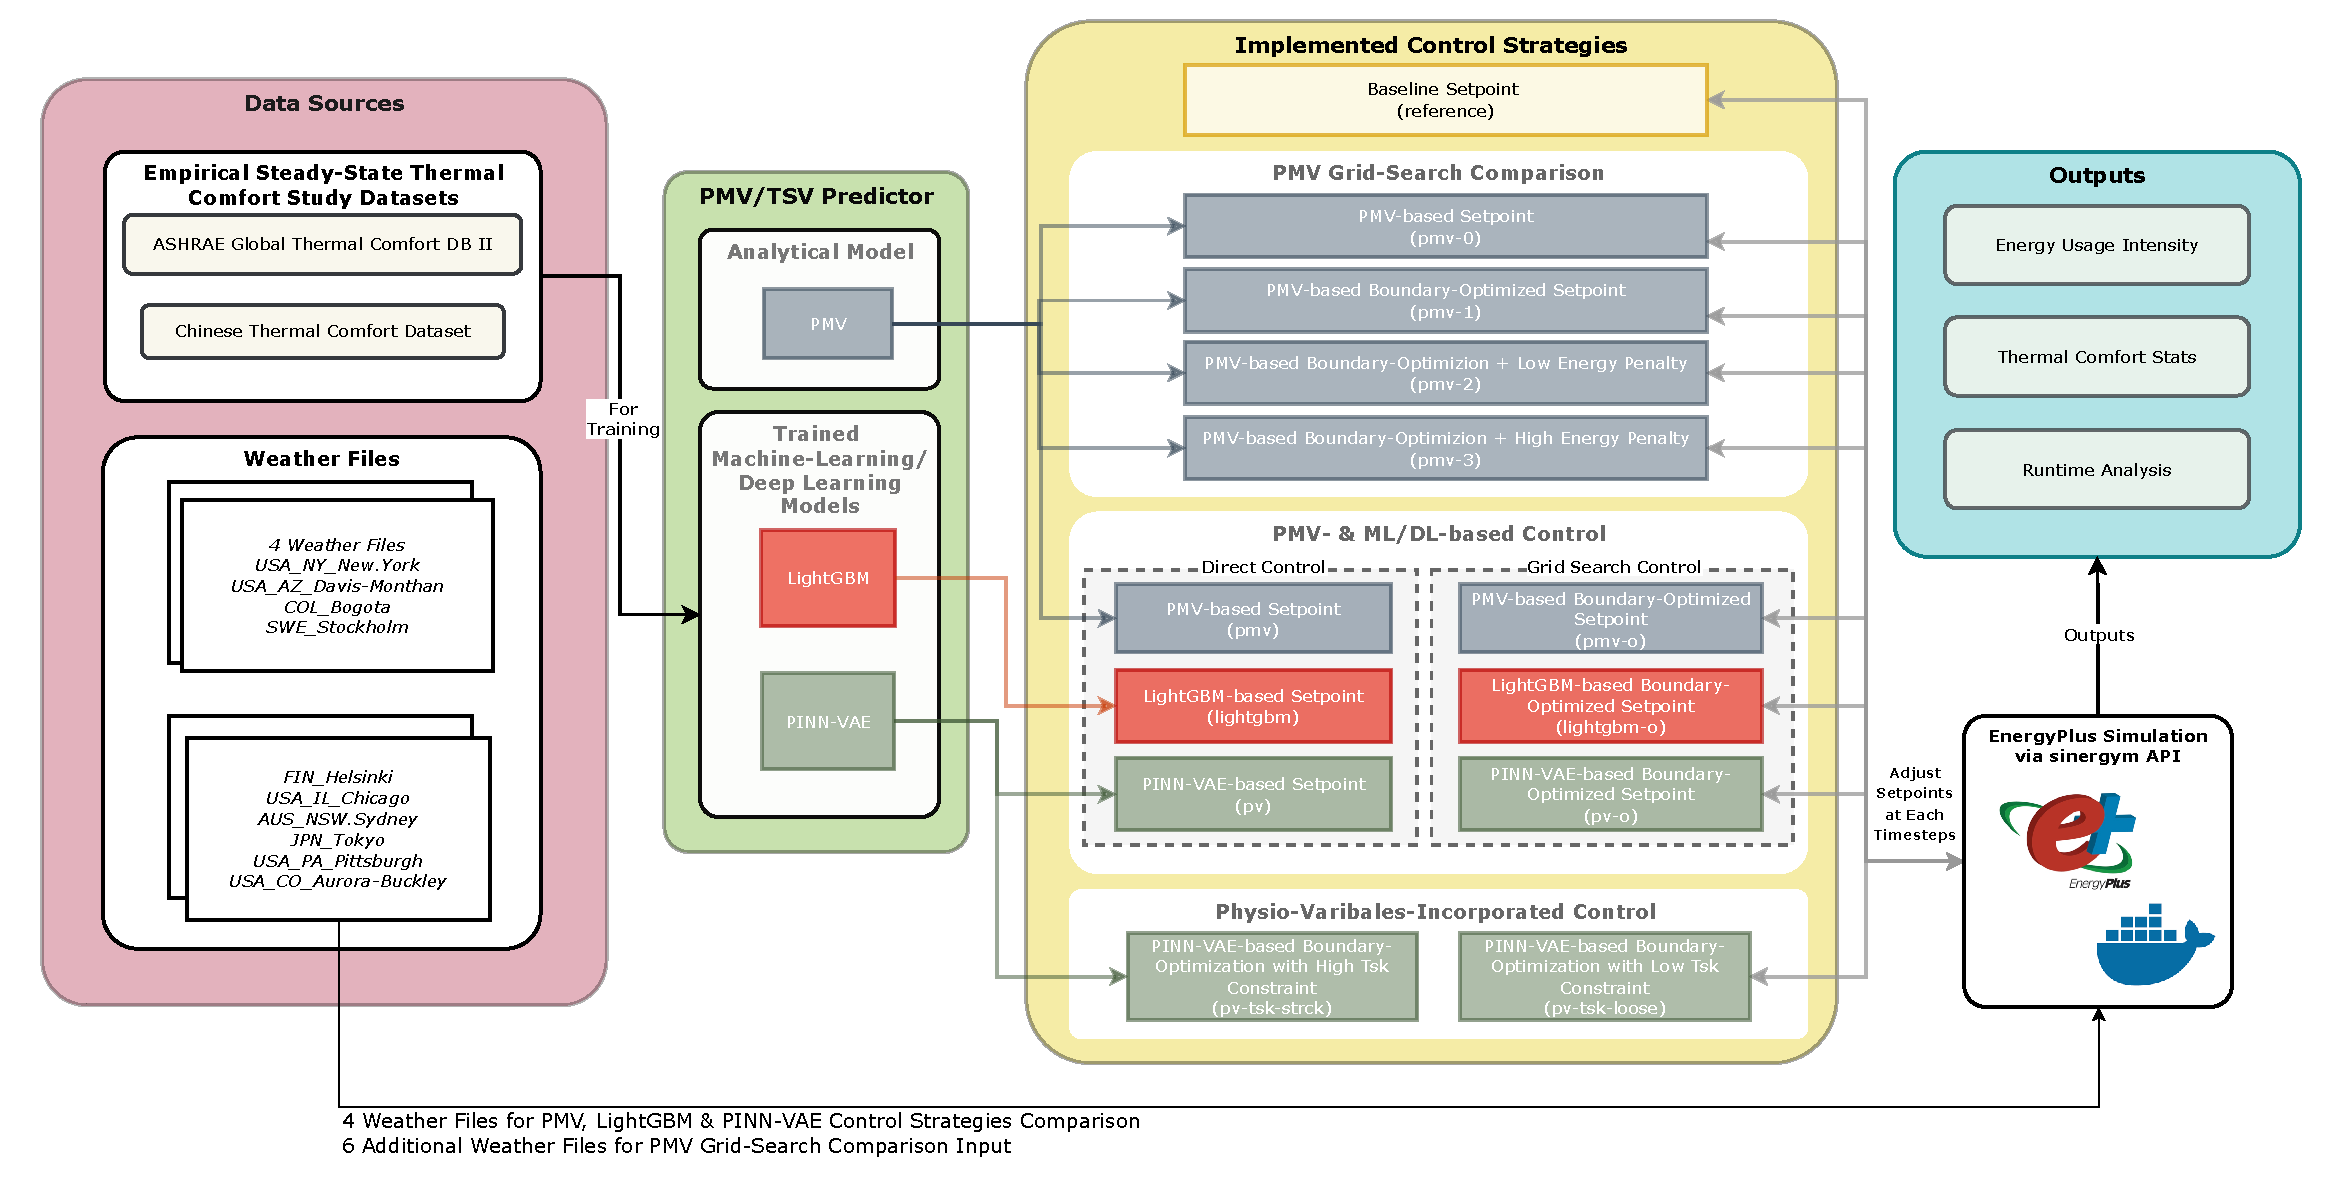
\includegraphics[width=0.95\linewidth]{figs/gridworkflow_3.pdf}
    \caption{Overall Workflow of Current Study}
    \label{fig:workflow}
\end{figure}

\subsection{Simulation Setup and Testbed Building}%Confirm we have enough on systems...?
% \subsubsection{Building Model Description and Justification}
This study adopts the \texttt{5ZoneAutoDXVAV} building model distributed with EnergyPlus \citep{energyplus}, which is commonly used for building control algorithm benchmarking \cite{gao2021deep, an2023clue, kadamala2024enhancing}. The model represents a single-story, 463 m$^2$ office building with five conditioned thermal zones and one return plenum, reflecting a prototypical open-plan office layout.

The building model supports zone-level temperature setpoint adjustment through Sinergym's actuator API, with the Energy Management System (EMS) framework enabling real-time control integration \cite{campoy2025sinergym}. We selected this model because it provides architectural symmetry and zoning simplicity that enable lightweight simulation environment and systematic algorithm testing, making it well-suited for comparative evaluation of different control strategies. While using a single building model limits generalizability to other building types and HVAC systems, this approach isolates performance differences attributable specifically to thermal comfort models and their climate interactions, rather than confounding variables from diverse building characteristics.


% \subsection{Envelope and Construction Details}
% The envelope construction is defined via abstracted \texttt{Construction} objects such as \texttt{WALL-1} and \texttt{ROOF-1}, though material layer specifications are absent in this JSON version. No window surface areas or window material properties are defined, and as such, the window-to-wall ratio (WWR) cannot be computed directly from this model. Nevertheless, the model's simplicity ensures consistent thermal response behavior and avoids geometric ambiguities \citep{drgovna2020all}.

% Each conditioned zone includes:
% \begin{itemize}
%   \item A \texttt{People} object representing occupancy density,
%   \item A \texttt{Lights} object simulating fixed lighting load, and
%   \item An \texttt{ElectricEquipment} object representing plug loads.
% \end{itemize}
% All internal gains are scheduled using \texttt{Schedule:Compact}, typically emulating business-hour profiles consistent with standard office operations. On top of that, the model includes:
% \begin{itemize}
%   \item A single \texttt{AirLoopHVAC} system with an outdoor air subsystem and return plenum (\texttt{PLENUM-1}),
%   \item Zone-level conditioning using VAV terminal units with DX cooling coils, and
%   \item Thermostat setpoint schedules that are designed to be overridden using external control via EMS actuators.
% \end{itemize}

% This setup supports cooling setpoint adjustment at the zone level, as exposed by Sinergym’s actuator API. The EMS framework facilitates real-time control from reinforcement learning agents without manual editing of EnergyPlus schedules or control logic.

% We selected this model for its:
% \begin{itemize}
%   \item \textbf{Representativeness}: Reflects the spatial and control complexity of a typical commercial office building;
%   \item \textbf{Simplicity}: Abstract geometry enables efficient simulation, particularly valuable for reinforcement learning experiments requiring thousands of rollouts;
%   \item \textbf{Modularity}: Provides a multi-zone testbed suitable for testing both centralized and decentralized control policies;
%   \item \textbf{Compatibility}: Fully integrated into the Sinergym ecosystem with predefined action and observation mappings \citep{perarnau2021sinergym};
%   \item \textbf{Reproducibility}: Used widely in prior RL-for-HVAC studies, including benchmarking efforts in \citep{gao2021deep}.
% \end{itemize}

% We understand the selection of a single IDF for this study may come with its own limitation, that the results we obtained will be specific to this building type and HVAC system. However, we believe a single, well-characterized IDF can help us isolate the performance differences that can be attributable solely to the model-enabled control strategies and their interactions with different climates, rather than variations in building systems/designs. %Reiterate this again in conclusions/discussions


\subsection{Data Source for Thermal Comfort Modeling} \label{sec:data_foundation}

As we're showing in Figure~\ref{fig:workflow}, the data source of the current study is a combination of both the ASHRAE Global Thermal Comfort Database II and the Chinese Thermal Comfort Datasets combined. This combined dataset represents a form of \textit{collective intelligence}, aggregated as 148,148 distinct pre-existing thermal sensation steady-state votes, encompassing both field and laboratory experiments from ASHRAE Thermal Comfort Database II and Chinese Thermal Comfort Datasets. This amalgamation results in a substantial corpus of 148,148 individual data points, capturing a wide diversity of environmental conditions, building typologies, geographical locations, and demographic profiles. 

The aggregation process involved careful harmonization of thermal sensation votes, typically reported on the 7-point ASHRAE scale, and standardization of input features to ensure consistency across the varied source studies. Further details on the construction, composition, and validation of this aggregated dataset can be found in [Dataset Paper Citation, if applicable, or a brief description of your harmonization process if not published separately]. This large-scale, diverse data foundation aims to foster the development of more generalized and robust thermal sensation models compared to those trained on smaller, single-source experimental data. Using this dataset, we were able to train both a machine learning (LightGBM) and deep learning (PINN-VAE, or physiological-informed neural net with variable autoencodeer) models for predicting thermal sensation are developed upon a comprehensive, aggregated dataset.

\subsection{Thermal Sensation Vote Predictors}\label{sec:comfort_models}
Aside from the analytical thermal sensation predictor of the population's mean thermal sensation, i.e. Predicted Mean Vote (PMV) \cite{Fanger1970}, we made explicit decisions on choosing the appropriate thermal sensation vote predictor. The selection process was guided by the dual objectives of robustness and innovation. We chose Light Gradient Boosting Machine (LightGBM) due to its consistently strong predictive performance with tabular datasets, as extensively validated in previous research\cite{Ke2017}. LightGBM offers computational efficiency, interpretability, and robust generalization capabilities, making it highly suitable for real-time predictive control tasks where reliability and speed are critical.

Concurrently, we introduce a novel Physics-Informed Neural Network combined with a Variational Autoencoder (PINN-VAE), specifically developed by the authors for thermal sensation prediction (publication forthcoming). This innovative model integrates physiological realism into thermal comfort modeling, explicitly leveraging Gagge's two-node model (Gagge et al., 1966) to analytically inform intermediate physiological outputs such as skin temperature ($T_{skin}$) and core body temperature ($T_{core}$). Unlike conventional predictive methods, the PINN-VAE architecture not only predicts thermal sensation with high fidelity through its deep neural network’s multi-head capability but simultaneously generates robust physiological data, significantly enhancing its utility in physiology-informed indoor environmental controls. This combination of predictive accuracy and physiological realism positions PINN-VAE as a potential transformative approach in building thermal environment management.

\subsubsection{Analytical Baseline: Predicted Mean Vote (PMV)}
\label{sec:pmv_model}
The Predicted Mean Vote (PMV) model, as developed by Fanger and standardized in ISO 7730 \citeplaceholder{ISO7730} and ASHRAE Standard 55 \citeplaceholder{ASHRAE55}, serves as an analytical baseline. PMV predicts the mean thermal sensation vote of a large group of people based on six key parameters: air temperature ($T_a$), mean radiant temperature ($T_r$), relative humidity ($RH$), air velocity ($v_{air}$), metabolic rate (Met), and clothing insulation ($I_{cl}$). In this study, when PMV-based control is active, these input parameters are derived from EnergyPlus outputs as observation of the environmental variables, coupled with predefined assumptions for occupant metabolic rate and clothing insulation, with more details documented in Section \ref{sec:control_strategies}.

We adopted standardized assumptions for occupant metabolic rates and clothing insulation based on established industry guidelines and widely accepted thermal comfort research. Specifically, a metabolic rate (MET) of 1.1 (sedentary office work) was used uniformly across simulations, consistent with recommendations by ASHRAE Standard 55\cite{ASHRAE2020}. Clothing insulation values (clo) were set to 0.65 during summer and 1.0 in winter, reflecting typical seasonal clothing variations commonly observed in office environments \cite{ASHRAE2020}.

These standardized assumptions facilitate reproducibility and enable direct comparability with established comfort models, such as PMV, while simultaneously aligning with typical office conditions documented in thermal comfort literature. Although using fixed values simplifies simulation procedures, we acknowledge potential limitations arising from the natural variability of individual occupant behavior and adaptive clothing choices in real-world scenarios.

\subsubsection{Machine Learning Benchmark: LightGBM}\label{sec:lightgbm_model}
A Light Gradient Boosting Machine (LightGBM) model is utilized as a high-performance machine learning benchmark for thermal sensation prediction. LightGBM is a tree-based gradient boosting framework known for its efficiency and accuracy \citeplaceholder{LightGBM\_Paper}. The model is trained on the aggregated dataset described in Section \ref{sec:data_foundation} to predict Thermal Sensation Vote (TSV) on the 7-point ASHRAE scale. Inputs to the LightGBM model include key environmental parameters such as [$T_a, T_r, RH, v_{air}$, clo, MET, gender, height, weight, etc.]. The model was trained using k-fold cross-validation, with hyperparameters optimized for predictive accuracy (details of training and validation are beyond the scope of this section but can be found in Appendix).

\subsubsection{Deep Learning Model: Physics-Informed Neural Network - Variational Autoencoder (PINN-VAE)}
\label{sec:pinn_vae_model}
The core novel model investigated in this study is a Physics-Informed Neural Network combined with a Variational Autoencoder (PINN-VAE), designed specifically for thermal sensation prediction and co-simulation of key physiological variables. This model architecture, detailed in a pending publication at BAE (will cite when publication is finalized), aims to overcome limitations of purely data-driven approaches by integrating domain knowledge such as physiological constraints on skin/core temperature, heat balance whilst improving the quality of input data that are missing.

In particular, the VAE component learns a robust latent representation of the input data, beneficial for handling the complexities and potential imperfections inherent in large-scale aggregated datasets. The PINN component incorporates physiological realism by embedding constraints derived from principles of human thermoregulation [e.g., based on a simplified Gagge's 2-node model \citeplaceholder{Gagge1966} or similar -- specify principles used, e.g., heat balance equations for core and skin compartments]. These physics-informed constraints guide the model to produce physiologically plausible predictions for mean skin temperature ($T_{skin}$) and core body temperature ($T_{core}$), alongside the primary output of TSV.

Inputs to the PINN-VAE are similar to the LightGBM model: [$T_a, T_r, RH, v_{air}$]. Its outputs for this study are the predicted TSV (on the 7-point ASHRAE scale), predicted $T_{skin}$, and predicted $T_{core}$. The key advantages of this PINN-VAE approach include its potential for improved generalization due to the physics-based regularization, enhanced interpretability through the prediction of intermediate physiological states, and the unique ability to leverage $T_{skin}$ as part of advanced control strategies. Training and validation details are provided in the aforementioned paper.

\section{Control Framework Implementation and Testing}
To demonstrate our co-simulation methodology's capabilities and assess its effectiveness, we implement seven distinct control strategies spanning analytical models to sophisticated deep learning approaches. This implementation serves multiple purposes: (1) confirming the framework successfully accommodates diverse model types and control logics, (2) testing the robustness of the actuator saturation handling and stochastic weather integration, and (3) generating initial insights into the relative performance of different comfort modeling approaches when deployed in actual control loops.

We emphasize that this section presents a systematic testing of our methodology rather than validation against measured building data—such empirical validation represents important future work once the framework's capabilities are established.

Our testing protocol comprises three complementary investigations:
\begin{itemize}
    \item PMV Grid-Search Optimization Study (Section 5.2): We first examine whether systematic optimization can enhance classical PMV control performance. Using 10 diverse climate locations, we compare naive PMV control against three grid-search variants to establish the potential of optimization for analytical models.
    \item Comprehensive Control Strategy Comparison (Section 5.3): We then apply our complete framework to compare seven control strategies—including both optimized and non-optimized variants of PMV, LightGBM, and PINN-VAE models—across four representative DOE climate zones. This investigation tests the framework's ability to fairly evaluate fundamentally different modeling approaches.
    \item Physiological Variable Integration (Section 5.4): Finally, we demonstrate the framework's extensibility by incorporating PINN-VAE's unique physiological predictions (skin temperature) into control logic, showcasing how our methodology enables novel control strategies beyond traditional comfort metrics.
\end{itemize}

\subsection{Control Strategies Tested}
\label{sec:control_strategies}
Across all three investigations, control strategies share common implementation characteristics. Despite their different internal logic, all controls implement a bang–bang adjustment of the heating and cooling set-points to be directly comparable against one another, with a maximum step of 1$^\circ$C per timestep (every 15 minutes). All modes share the following pre-processing steps:

\begin{itemize}
  \item \textbf{Occupancy check:} The space is considered unoccupied if it is a weekend day or outside the hours of 06:00–22:00. In unoccupied periods, the allowable comfort range is relaxed by \(\pm\SI{2}{\degreeCelsius}\).
  \item \textbf{Seasonal set‐points:} Two baseline comfort ranges, \(\left[T_\mathrm{low}^\mathrm{sum},T_\mathrm{high}^\mathrm{sum}\right]\) for summer (June 1–September 30) and \(\left[T_\mathrm{low}^\mathrm{win},T_\mathrm{high}^\mathrm{win}\right]\) for the remainder of the year, are defined a priori.  
  \item \textbf{Environmental inputs:} At each timestep, the current air temperature \(T_a\), relative humidity RH, and mean radiant temperature \(T_r\) are read from the observation vector.  
\end{itemize}

\subsubsection{Baseline Control (reference)}
\label{sec:reference_control}
The reference controller adjusts set-points based solely on the air temperature relative to the comfort range. Let
\[
(T_\mathrm{low},\,T_\mathrm{high}) = 
\begin{cases}
(T_\mathrm{low}^\mathrm{sum},\,T_\mathrm{high}^\mathrm{sum}), & \text{summer},\\
(T_\mathrm{low}^\mathrm{win},\,T_\mathrm{high}^\mathrm{win}), & \text{winter},
\end{cases}
\]
expanded by \(\pm2\)\,$\degree$C if unoccupied. Denote the current heating and cooling set‐points by \(T_\mathrm{htg}\) and \(T_\mathrm{clg}\). Then:
\begin{equation}
\begin{aligned}
\text{if } T_a &< T_\mathrm{low}: & T_\mathrm{htg}&\leftarrow T_\mathrm{htg}+1,\quad T_\mathrm{clg}\leftarrow T_\mathrm{clg}+1,\\
\text{if } T_a &> T_\mathrm{high}: & T_\mathrm{htg}&\leftarrow T_\mathrm{htg}-1,\quad T_\mathrm{clg}\leftarrow T_\mathrm{clg}-1,\\
\text{otherwise:} & & T_\mathrm{htg},\,T_\mathrm{clg}&\text{ unchanged.}
\end{aligned}
\end{equation}

\subsubsection{PMV-Based Setpoint Control (pmv)}
\label{sec:pmv_control}
The PMV controller uses the predicted Predicted Mean Vote (PMV) from the \texttt{pmv\_ppd\_iso} function, computed over the current conditioned air state. We define
\[
\mathrm{PMV} = f_\mathrm{ISO}\bigl(T_a,\,T_r,\,\mathrm{RH},\,\mathrm{met}=1.1,\,\mathrm{clo}\bigr),
\]
where \(\mathrm{clo}=0.65\) in summer and \(1.0\) in winter (adjusted for unoccupied periods as above). Denoting the mean PMV by \(\overline{\mathrm{PMV}}\), the set-point adjustment is
\begin{equation}
\begin{aligned}
\text{if } \overline{\mathrm{PMV}} &< -0.5: & T_\mathrm{htg}&\leftarrow T_\mathrm{htg}+1,\quad T_\mathrm{clg}\leftarrow T_\mathrm{clg}+1,\\
\text{if } \overline{\mathrm{PMV}} &> +0.5: & T_\mathrm{htg}&\leftarrow T_\mathrm{htg}-1,\quad T_\mathrm{clg}\leftarrow T_\mathrm{clg}-1,\\
\quad \quad & \text{otherwise:} & & T_\mathrm{htg},\,T_\mathrm{clg} \text{ unchanged.}
\end{aligned}
\end{equation}

Both controllers’ outputs \((T_\mathrm{htg},\,T_\mathrm{clg})\) are clipped to the environment’s allowable action space before being sent to EnergyPlus. These two modes serve as benchmarks against which we compare our ML­-enhanced and grid-search optimized strategies.

\subsubsection{LightGBM- and PINN-VAE- Based Control (lightgbm \& pv)}
\label{sec:lightgbm_control}

The two ML/DL-based controllers use our pre‐trained Gradient Boosting model (lightgbm) and PINN-VAE model (pv) respectively to predict the proxy occupants’ Thermal Sensation Vote (TSV) and applies a simple bang–bang adjustment of the HVAC set‐points. At each timestep, the following procedure is executed:

\begin{enumerate}
  \item \textbf{Feature assembly.} Construct a feature vector (or matrix) \(\mathbf{x}\) containing the current indoor air temperature \(T_a\), relative humidity RH, mean radiant temperature \(T_r\), clothing insulation (\(\mathrm{clo}\)), etc., exactly as in Section~\ref{sec:control_strategies}.
  \item \textbf{TSV prediction.}  
    \[
      \widetilde{\mathrm{TSV}} = \mathrm{ModelWrapper.predict}(\mathbf{x}),
    \]
    where \(\widetilde{\mathrm{TSV}}\in\mathbb{R}^n\) (one prediction per zone or sample).  
  \item \textbf{Aggregate comfort metric.} Compute the median sensation vote:
    \[
      \mathrm{TSV}_{\mathrm{med}} = \mathrm{median}\bigl(\widetilde{\mathrm{TSV}}\bigr).
    \]
  \item \textbf{Bang–bang set‐point update.} Let \(T_{\mathrm{htg}}\) and \(T_{\mathrm{clg}}\) be the current heating and cooling set‐points. Then
    \[
    \begin{cases}
      T_{\mathrm{htg}} \leftarrow T_{\mathrm{htg}} + 1,\quad
      T_{\mathrm{clg}} \leftarrow T_{\mathrm{clg}} + 1, 
      & \text{if } \mathrm{TSV}_{\mathrm{med}} < -0.5,\\[6pt]
      T_{\mathrm{htg}} \leftarrow T_{\mathrm{htg}} - 1,\quad
      T_{\mathrm{clg}} \leftarrow T_{\mathrm{clg}} - 1, 
      & \text{if } \mathrm{TSV}_{\mathrm{med}} > +0.5,\\[6pt]
      \text{unchanged,} & \text{otherwise.}
    \end{cases}
    \]
  \item \textbf{Clipping.} Finally, clip \((T_{\mathrm{htg}},T_{\mathrm{clg}})\) to the environment’s allowable action‐space.
\end{enumerate}

\noindent\emph{Computational considerations:}  
Because the wrapper instantiates a LightGBM model and meta‐information only once per episode (caching column order, category mappings, etc.), the per‐timestep cost is dominated by a single vectorized predict call, \(\mathcal{O}(n)\) in the number of samples. Memory overhead is negligible for typical zone counts (\(n<10\)).


\subsubsection{Boundary-Optimized Control (pmv-o, lightgbm-o \& pv-o)}
\label{sec:opt_boundary_pseudocode}

All boundary modes perform the same grid-search over a set of temperature offsets \(\Delta T\) to drive the predicted comfort metric as close as possible to the comfort boundaries \(\pm0.5\). The PMV or TSV values are predicted with different prediction models, i.e., PMV, LightGBM and PINN-VAE (abbreviated hereinafter as pmv-o, lightgbm-0 and pv-o). We summarize the procedure in Algorithm~\ref{alg:boundary_opt}.

\begin{algorithm}[ht]
\caption{Boundary‐Optimized Set‐Point Adjustment}\label{alg:boundary_opt}
\KwIn{Current features $\mathbf{x}$, set‐points $(T_\text{htg},T_\text{clg})$, predictor $\mathsf{pred}(\cdot)$}
\KwData{Shifts $\mathcal{D}=\{-2,\dots,2\}$}
Build batch $\mathbf{X}\leftarrow[\mathbf{x}+\delta_1;\dots;\mathbf{x}+\delta_m]$\;
$\mathbf{y}\leftarrow\mathsf{pred}(\mathbf{X})$\;
Reshape into $\mathbf{Y}\in\mathbb{R}^{m\times n}$\;
\For{$i\leftarrow1$ \KwTo $m$}{
  $s_i^-\leftarrow|\mathrm{med}(\mathbf{Y}_i)+0.5|$\;
  $s_i^+\leftarrow|\mathrm{med}(\mathbf{Y}_i)-0.5|$\;
}
$\delta^-\leftarrow\arg\min_i s_i^-$; $\delta^+\leftarrow\arg\min_i s_i^+$\;
$\delta^*\leftarrow\arg\min_{\delta\in\{\delta^-,\delta^+\}}|\delta|$\;
$T_\text{htg}\mathbin{+{\mkern-8mu}=}\delta^*$; $T_\text{clg}\mathbin{+{\mkern-8mu}=}\delta^*$\;
Clip to action space\;
\end{algorithm}

Because we reset any extreme setpoints to (19$^\circ$C, 27$^\circ$C) before evaluating ∆T, none of the candidate shifts (\pm2$^\circ$C, \pm1$^\circ$C, \pm0.5$^\circ$C) ever crosses the hard bounds [12$^\circ$C, 23.25$^\circ$C]×[23.25$^\circ$C, 30$^\circ$C], thereby eliminating actuator saturation in the grid-search process.
\noindent\emph{Practical considerations:}  
The single batch predict call reduces overhead compared to looping over shifts. Total complexity remains \(\mathcal{O}(mn)\) model evaluations, with memory to hold \(m\!n\) feature rows. In our experiments (\(m=9,n<10\)), this executes in under 150\,ms per timestep, making it suitable for real‐time or near‐real‐time HVAC control loops.

\subsubsection{Physiological Variables Incorporated Boundary-Optimized Control (pv-tsk-strick \& pv-tsk-loose)}
\label{sec:pv_tsk_control}
The PINN-VAE model, with its intrinsically physiological-constrained model design, is capable of predicting physiological variables, including skin temperature ($T_{skin}$), apart from TSV value. Built upon the aforementioned boundary-optimized PINN-VAE control strategy (\texttt{pv-o}), we further incorporate the predicted $T_{skin}$ into control strategy to better leverage the capacities of the advanced model. Specifically, at each action point, the agent evaluates whether both the predicted TSV and $T_{skin}$ falls within the target range while maintaining the same grid search strategy to find the minimum setpoint deviation that meet the both criterion (\texttt{pv-tsk-strict}). Alternatively, as a more relaxed control strategy, the comfort requirement is considered to be met if either the TSV or $T_{skin}$ falls within its respective comfort range (\texttt{pv-tsk-loose}). The $T_{skin}$ target range is set at a conservative comfort range $32.8\,^\circ\mathrm{C} \leq T_{skin} \leq 33.8\,^\circ\mathrm{C}$ as reported by Weiwei et al. \cite{liuUseMeanSkin2015}. Since pv-o itself never generates clipped setpoints, these pv-tsk variants likewise avoid any actuator saturation.

\subsection{Inputs and Outputs}
\paragraph{Weather Files used}\label{sec:weather_noise}
We employed twelve EPW-format weather files as the nominal dataset for year-long EnergyPlus simulations\footnote{Typical EPW fields and structure are defined in the EnergyPlus Weather File Data Dictionary\cite{EPW_Data_Dictionary}}.  
From these, four representative files—selected according to DOE climate zone classifications (e.g., 2B: hot‐dry; 4A: mixed‐humid; 5C: cool‐marine; 7: cold)—were used to benchmark the control strategies outlined in Section~\ref{sec:control_strategies}.  

An additional eight EPW files were reserved for extended validation of PMV-based set‐point optimization. To account for meteorological variability and reinforce the robustness of our findings, we enabled the stochastic weather module in the Sinergym package, which injects Gaussian perturbations (zero mean, $\sigma$ = 2.5 $\degree$C) into the dry-bulb and radiant temperature series for each timestep\cite{Sinergym_Stochastic}.


This stochastic weather module is critical for establishing the statistical robustness of our findings. Rather than evaluating control performance under a single deterministic weather year—which could lead to overfitting to specific weather patterns—each simulation experiences unique weather realizations. The Gaussian perturbations ($\sigma$ = 2.5°C) applied to dry-bulb and radiant temperatures at every timestep ensure that our control strategies are tested against a distribution of possible weather conditions, not just historical averages. This approach inherently provides statistical validation by demonstrating that the performance rankings and energy savings remain consistent despite weather variability, strengthening confidence in the generalizability of our results.
\begin{itemize}
  \item \textbf{EPW format:} Comma-delimited with hourly records for 8,760 hours, containing standard fields such as Year, Month, Day, Hour, Dry-Bulb Temperature, and Sky Infrared Radiation\cite{EPW_Format}.
  \item \textbf{Climate selection:} Four climates (2B, 4A, 5C, 7) chosen to span hot-dry, mixed-humid, cool-marine, and cold conditions.
  \item \textbf{Stochastic noise:} Gaussian noise ($\mu$=0, $\sigma$=2.5 $\degree$C) added to temperature fields via Sinergym’s stochastic environments\cite{Sinergym_Stochastic}, enhancing sensitivity analysis and result stability.
\end{itemize}

\paragraph{Performance Metrics (Overview)}
To compare the different control strategies (reference, PMV, LightGBM, PINN-VAE and optimized variants), we will evaluate the outputs from the EnergyPlus simulation across:  
\begin{itemize}
  \item Annual energy consumption by end use types (and percent savings relative to the reference), on top of energy usage intensitivies.  
  \item Fraction of occupied hours with TSV within the $\pm$0.5 comfort/thermal neutral band.  
  \item Average simulation runtime per annual run.  
\end{itemize}
The results of the comparison of these metrics across different runs are reported in the results section of this paper and further discussed in corresponding discussion sections.%Add more?
The precise mathematical definitions and any additional robustness or combined‐FoM (Combined Figure of Merit) metrics are given in Section~\ref{sec:performance_metrics}.%? I guess perhaps add some more to appendix?


\subsection{Actuator Limits and Saturation Considerations}
\label{sec:actuator_saturation_method}

In \texttt{5ZoneAutoDXVAV} example file, the default heating and cooling setpoints are hard‐limited beyond the EnergyPlus allowable range to
\[
12\,^\circ\mathrm{C} \;\leq T_{h} \;\leq 23.25\,^\circ\mathrm{C} 
\quad\text{and}\quad
23.25\,^\circ\mathrm{C} \;\leq T_{c} \;\leq 30\,^\circ\mathrm{C}.
\]
Whenever a controller requests a setpoint outside these bounds, Sinergym automatically clips it to the nearest limit—a phenomenon we refer to as \emph{actuator saturation}. If left unaddressed, any logic that naively drives $T_{h}<12\,^\circ\mathrm{C}$ or $T_{c}>30\,^\circ\mathrm{C}$ will simply “stick” at the boundary, masking the true comfort–energy trade‐off.

In our initial “pure” implementations (PMV inversion, LightGBM inversion, PV inversion), we observed that repeated attempts to push setpoints beyond $12\,^\circ\mathrm{C}$ or $30\,^\circ\mathrm{C}$ yielded clipped controls that never returned to an interior value. To mitigate this, we introduced a boundary‐optimized grid‐search protocol as follows:  
\begin{enumerate}
  \item \textbf{Interior Reset.} Whenever the previous setpoint pair $(T_{h},T_{c})$ falls outside $[13\,^\circ\mathrm{C},29\,^\circ\mathrm{C}]$, we immediately reset to $(19\,^\circ\mathrm{C},\,27\,^\circ\mathrm{C})$.  
  \item \textbf{$\Delta T$ Grid Search.} From that interior point, we evaluate seven candidate offsets
    \[
      \Delta T \;\in\; \{-2.0,\,-1.0,\,-0.5,\,0.0,\,+0.5,\,+1.0,\,+2.0\}\,\text{°C}
    \]
    simultaneously. Because $(19\,^\circ\mathrm{C} \pm 2\,^\circ\mathrm{C})$ and $(27\,^\circ\mathrm{C} \pm 2\,^\circ\mathrm{C})$ lie strictly within the allowable $[12\,^\circ\mathrm{C},\,30\,^\circ\mathrm{C}]$ band, none of these candidates are ever clipped.  
  \item \textbf{Final Gap Enforcement.} After selecting the best $\Delta T$ (based on $\bigl|\lvert \text{comfort}\rvert - 0.5\bigr|$ plus an energy penalty), we reimpose a $2\,^\circ\mathrm{C}$ heating–cooling gap and then perform one last clamp to guarantee feasibility.  
\end{enumerate}

By acknowledging Sinergym’s actuator saturation up front and embedding this reset + $\Delta T$ grid logic in the methodology, we ensure that none of our “optimized” setpoints are artifactual products of clipping. This approach eliminates “sticking” at $12\,^\circ\mathrm{C}$ or $30\,^\circ\mathrm{C}$ and preserves a meaningful comfort gradient throughout the simulation.
\section{Results}

\subsection{Simulation Results Overview}
All results presented represent performance under stochastic weather conditions, with each simulation experiencing unique perturbations to the baseline weather data. This ensures our findings reflect robust performance across weather variability rather than optimization to specific weather patterns. The co-simulations are conducted through 3 categories of control strategies, corresponding to our specific research focus as outlined as follows:
\begin{itemize}
    \item \textbf{PMV-based}: Applying variants with different regulating methods and energy penalty to fully exploring the potential of PMV as an analytical model in building control.
    \item \textbf{PMV- \& ML-based variants}: Introducing LightGBM and PINN-VAE predicted TSV as controlling metic to further compare the performance of various models and the tradeoff in computation resources.
    \item \textbf{PV-based}: Incorporating $T_{skin}$ as additional constraint as a preliminary attempt to integrate physiological variables into HVAC control.
\end{itemize}
The percentage change in EUI compared to \texttt{reference} of all control strategies are shown in Table~\ref{tab:overview_results}. The $T_{skin}$-involved strategies are compared to \texttt{pv-o} rather than \texttt{reference}, since the objective is not to evaluate control performance per se, but to investigate the viability of integrating physiological indicators into the control framework as further explained in Section~\ref{sec:tsk_results}. As we show in Section 5.3.1, both LightGBM‐ and PV‐only variants frequently saturate at 12 $^\circ$C or 30 $^\circ$C, which artificially depresses their reported EUI values; Section~\ref{sec:tsk_results} will quantify this saturation.

\begin{table}[htbp]
\centering
\small % Reduce font size for the entire table
\caption{Overview of Percentage Change in Energy Use Intensity (EUI) for Different Control Strategies Compared to `reference' Control}
\label{tab:overview_results}
\setlength{\tabcolsep}{4pt}
\begin{tabularx}{\textwidth}{llXr}
\toprule
\textbf{Category} & \textbf{Name} & \textbf{\makecell{Description\\(model + method + extra)}} & \textbf{\makecell{EUI\\(\%)}} \\
\midrule

\multirow{4}{*}{PMV-based} 
  & pmv-0 & PMV + Bang-bang adjustment                        & 11.23\% \\
  & pmv-1 & PMV + Boundary-optimization                       & \textbf{-12.75}\% \\
  & pmv-2 & PMV + Boundary-optimization + Low energy penalty  & -12.66\% \\
  & pmv-3 & PMV + Boundary-optimization + High energy penalty & -12.52\% \\

\midrule
\multirow{6}{*}{\makecell{PMV- \& ML- \\ based variants} } 
  & pmv         & PMV + Bang-bang adjustment (same as pmv-0)     & 11.23\% \\
  & lighgbm     & LightGBM + Bang-bang adjustment                & 24.48\% \\
  & pv          & PINN-VAE + Bang-bang adjustment                & 19.13\% \\
  & pmv-o       & PMV + Boundary-optimization (same as pmv-1)    & -7.96\% \\
  & lightgbm-o  & LightGBM + Boundary-optimization               & -7.45\% \\
  & pv-o        & PINN-VAE + Boundary-optimization               & \textbf{-9.49}\% \\

\midrule
\multirow{2}{*}{PV-based} 
  & pv-tsk-strict & PINN-VAE + Boundary-optimization + Strict $T_{skin}$ constraint & 1.97\% \\
  & pv-tsk-loose  & PINN-VAE + Boundary-optimization + Loose $T_{skin}$ constraint  & -0.09\% \\

\bottomrule
\end{tabularx}
\vspace{1.0em} % Add some space before the note
\begin{minipage}{\linewidth}
\footnotesize\raggedright
\textit{Note:} 1. The EUI(\%) values in PMV-based and PMV- \& ML- based variants categories reflects the mean of percentage changed compared to their `reference' control strategy across four cities compared, values reported in `PV-based' category represent percentage change compared to \texttt{pv-o} strategy.\\
2. The EUI(\%) values in PMV-based category is averaged through 10 various cities/sites as outlined in Section~\ref{sec:pmv_results}, while the values in PMV- \& ML- based variants and PV-based categories are averaged through 4 cities/sites as outline in Section~\ref{sec:all_control_strategies}. \\
3. Positive values indicate an increase in EUI; negative values signify a decrease (energy savings).
\end{minipage}
\end{table}

\subsection{PMV-Grid-Search: Energy and Comfort Implications}
\label{sec:pmv_results}
The study investigates the impact of various Predicted Mean Vote (PMV)-driven HVAC optimization strategies on energy consumption compared to a standard bang-bang control (`reference`). The results in Table~\ref{tab:pmv_results}, showcasing percentage changes in Energy Use Intensity (EUI), are analyzed across ten diverse global locations. We evaluated control performance across four representative climate categories—Temperate Oceanic (Sydney, Australia), Humid Continental (Stockholm, Sweden), Subtropical Highland (Bogotá, Colombia), and Humid Subtropical (New York, USA)—supplemented by eight additional sites (e.g., Helsinki, Chicago, Tokyo, Davis-Monthan AFB) to ensure robustness under diverse heating, cooling, and humidity loads.  

\begin{table}[htbp]
\centering
\small % Reduce font size for the entire table
\caption{Percentage Change in EUI for PMV Optimization Strategies Compared to Reference Bang-Bang Control, and General Climate Classifications.}
\label{tab:pmv_results}
% Adjust \tabcolsep for better spacing
\setlength{\tabcolsep}{4pt}
% Use tabularx to make the table fit within \textwidth
\begin{tabularx}{\textwidth}{@{} l >{\raggedright\arraybackslash}X c c c c >{\raggedright\arraybackslash}X @{}}
\toprule
\makecell[l]{City/\\Site} & \makecell[l]{Climate Type\\(General)} & \makecell{pmv0\\(\%)} & \makecell{pmv1\\(\%)} & \makecell{pmv2\\(\%)} & \makecell{pmv3\\(\%)} & \makecell[l]{Uncovered\\Savings}\\
\midrule
Sydney       & Temperate Oceanic        & 4.30  & $-18.47$ & $-18.08$ & $-18.13$ & Significant  \\
Helsinki     & Humid Continental        & 21.44 & $-17.85$ & $-18.00$ & $-17.40$ & Significant  \\
Bogota       & Subtropical Highland     & 11.33 & $-15.52$ & $-15.55$ & $-15.33$ & Significant  \\
Stockholm    & Humid Continental        & 23.53 & $-15.31$ & $-15.75$ & $-15.62$ & Significant  \\
Antananarivo & Subtropical Highland     & 6.08  & $-15.29$ & $-15.05$ & $-14.94$ & Significant  \\
Chicago      & Humid Continental        & 22.00 & $-11.40$ & $-11.14$ & $-11.13$ & Consistent   \\
Pittsburgh   & Humid Continental        & 20.50 & $-10.08$ & $-10.05$ & $-9.75$  & Consistent   \\
Davis-Monthan& Hot Desert               & 7.68  & $-8.61$  & $-8.30$  & $-8.18$  & Consistent   \\
New York     & Humid Subtropical        & 20.45 & $-7.97$  & $-8.06$  & $-7.91$  & Consistent   \\
Tokyo        & Humid Subtropical        & 20.06 & $-7.01$  & $-6.65$  & $-6.78$  & Consistent   \\
\bottomrule
\end{tabularx}
\vspace{0.7em} % Add some space before the note
% {\footnotesize\textit{Note:} The values in pmv0 through pmv3 represent the percentage change in EUI relative to the reference control strategy (value of 0.0). Positive values indicate an increase in EUI; negative values signify a decrease (energy savings).}
\end{table}


\begin{figure}[h!]
    \centering
    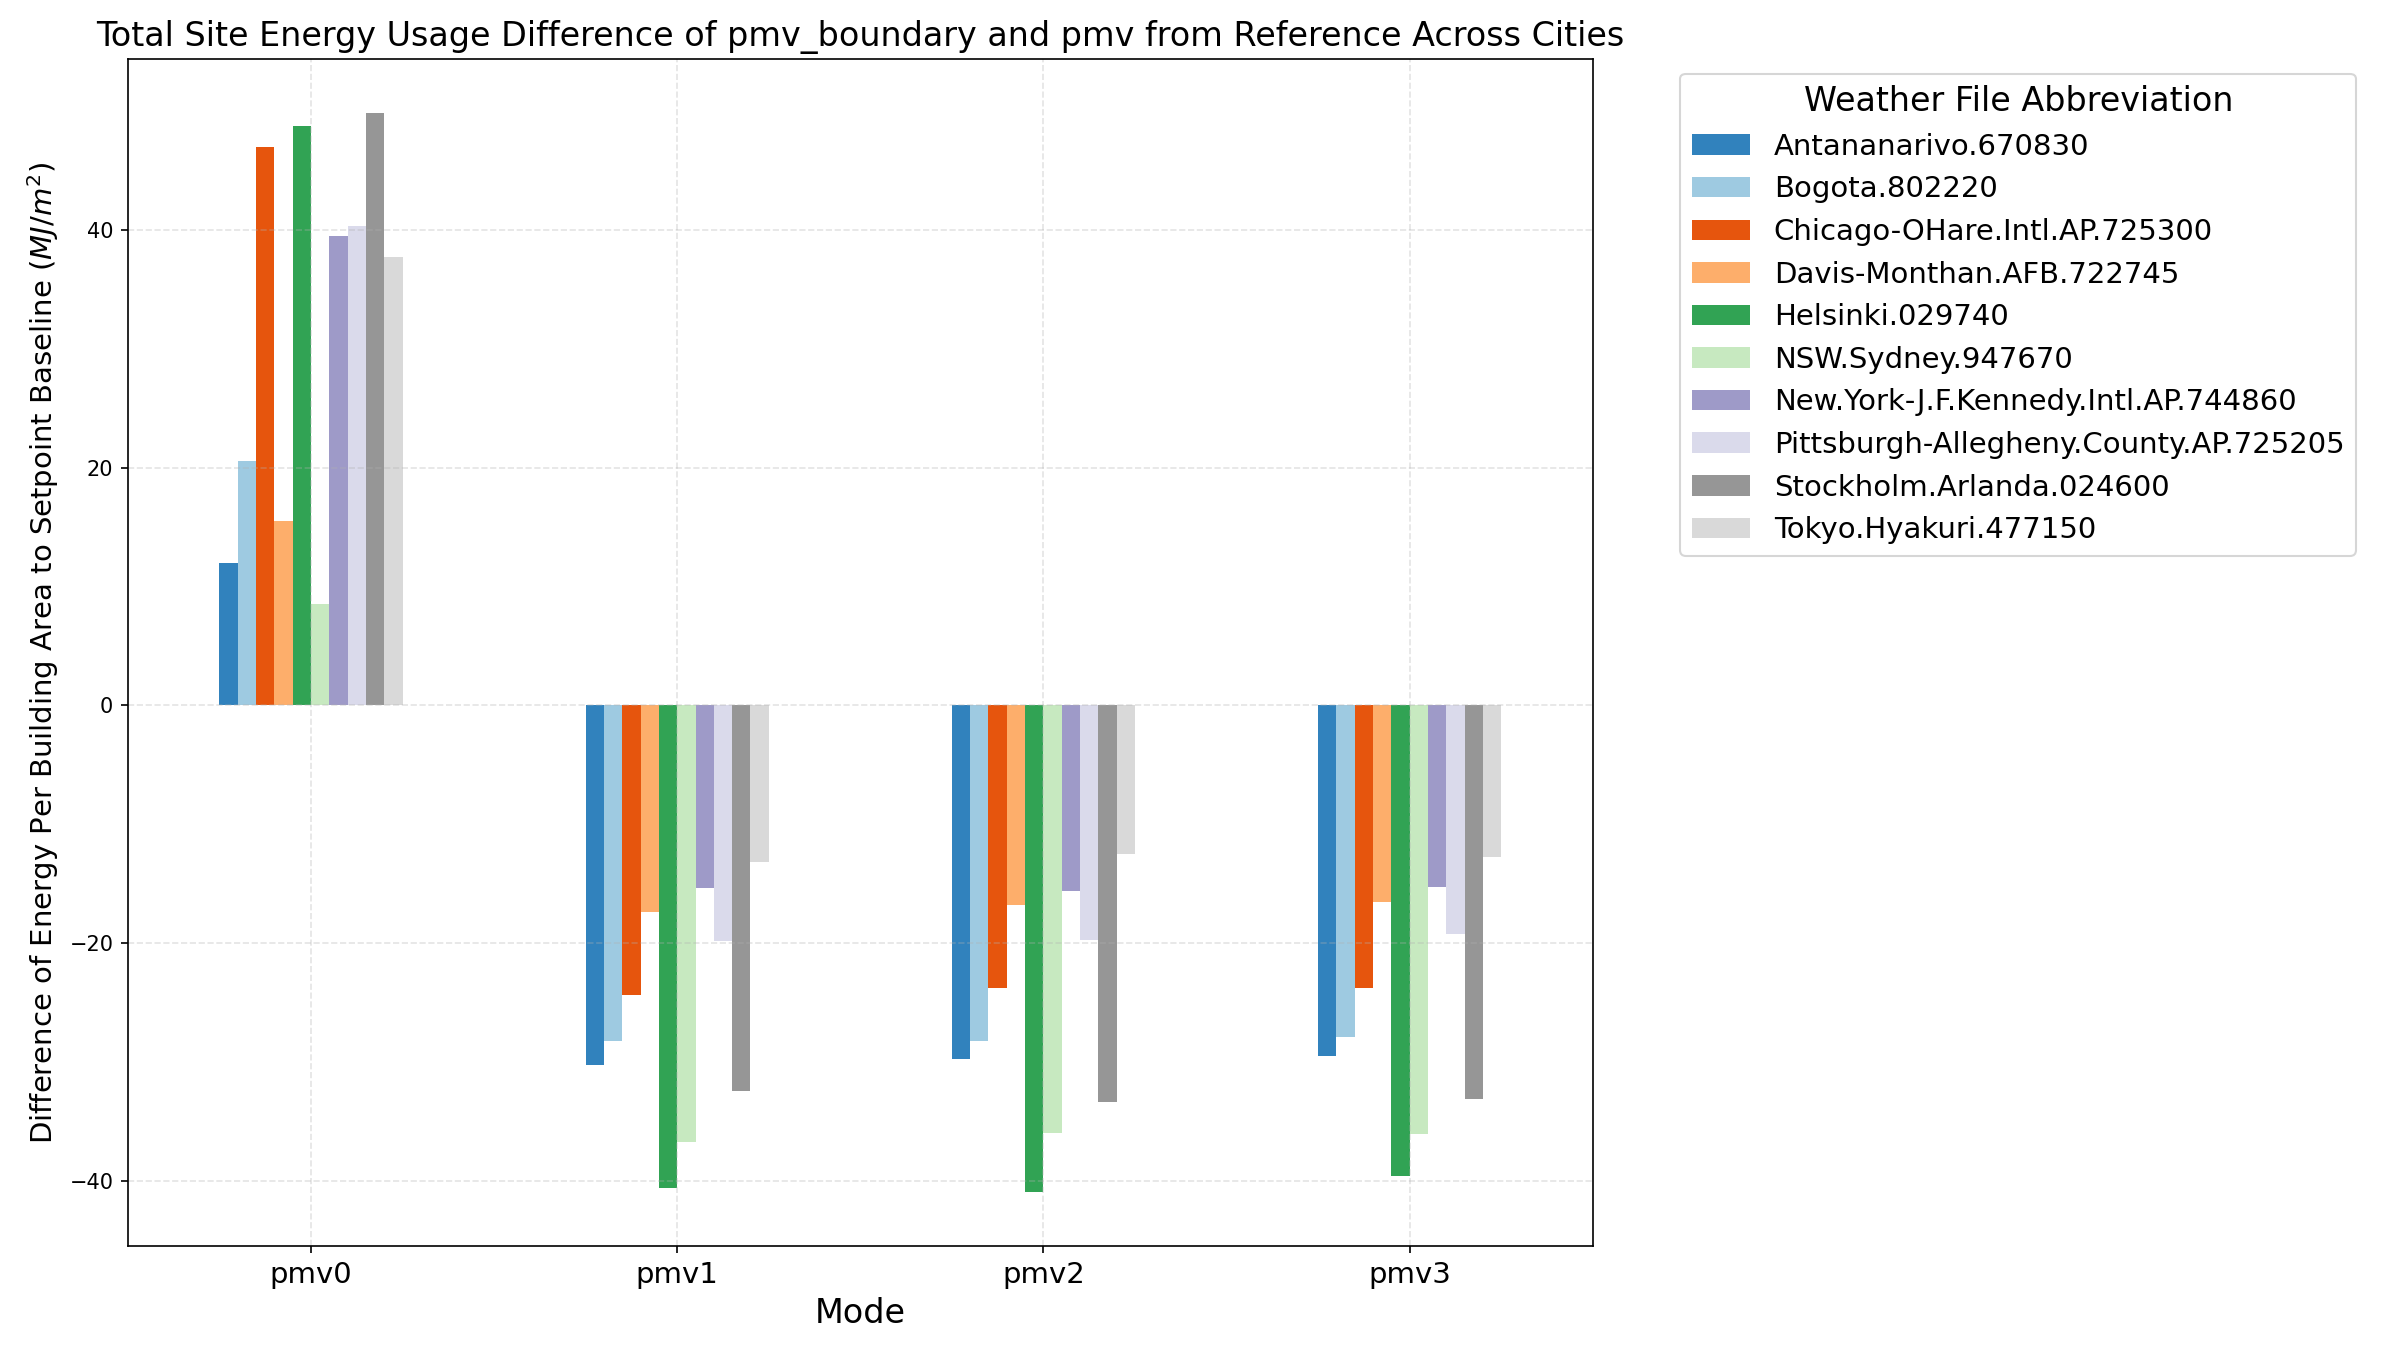
\includegraphics[width=0.85\linewidth]{figs/pmv_search_weather.png}
    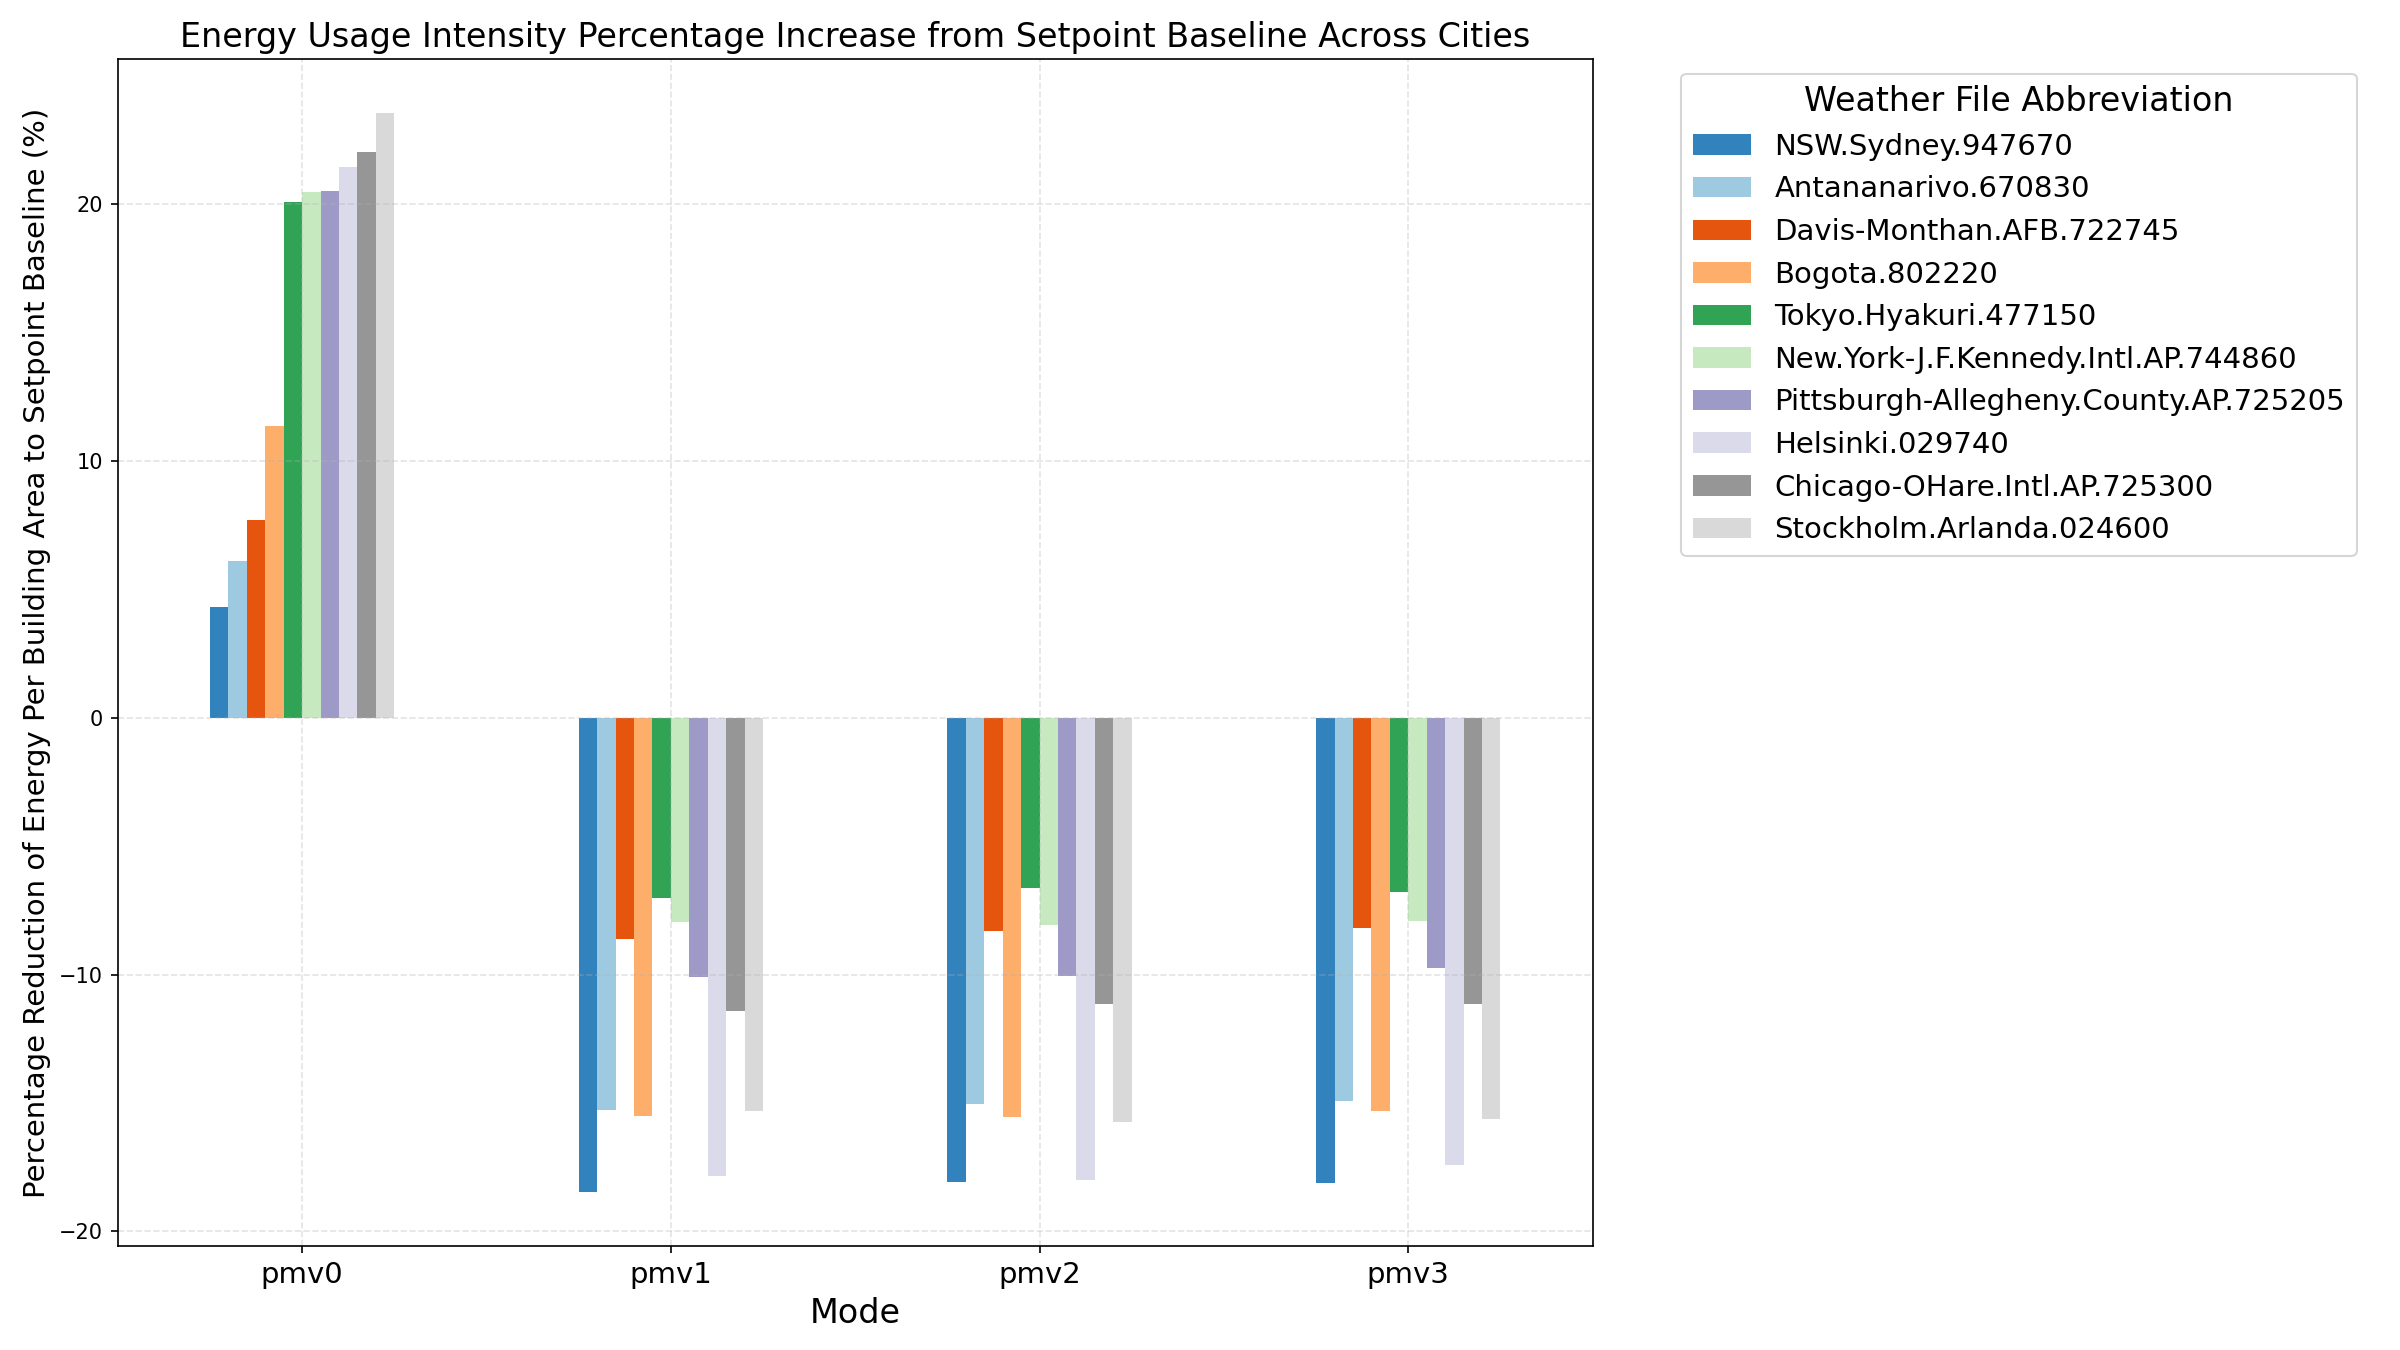
\includegraphics[width=0.85\linewidth]{figs/pmv_search_weather_perc.png}
    \caption{Energy Usage Intensity from EnergyPlus Simulations across multiple weather files (as specified with Figure~\ref{fig:workflow}}
    \label{fig:pmv-grid}
\end{figure}


\subsubsection{Observed Energy Savings with Grid-Search PMV Optimization}

In contrast to \texttt{pmv0}, the PMV-driven strategies employing grid-search optimization (\texttt{pmv1}, \texttt{pmv2}, \texttt{pmv3}), which incorporate different weightings for the energy/comfort trade-off and varied setpoint adjustment step sizes, demonstrated considerable success in reducing energy consumption relative to the bang-bang control.
\paragraph{Significant Savings (approx. 15\% to 18.5\% reduction):} Locations such as Helsinki ($ \approx -17.4\% \text{ to } -18.0\%$), Stockholm ($ \approx -15.3\% \text{ to } -15.8\%$), Sydney ($ \approx -18.1\% \text{ to } -18.5\%$), Bogota ($ \approx -15.3\% \text{ to } -15.6\%$), and Antananarivo ($ \approx -14.9\% \text{ to } -15.3\%$) fall into this category. These results are particularly prominent in climates with substantial heating seasons (Helsinki, Stockholm) but are also evident in the temperate oceanic climate of Sydney and the cooler subtropical highland climates. This suggests that intelligent PMV control can effectively capitalize on opportunities for energy reduction in varied conditions, possibly by optimizing system operation during significant heating/cooling periods or leveraging favorable ambient conditions in milder climates.

\paragraph{Consistent Savings (approx. 7\% to 11.5\% reduction):} Cities like Chicago ($ \approx -11.1\% \text{ to } -11.4\%$), Pittsburgh ($ \approx -9.8\% \text{ to } -10.1\%$), Davis-Monthan AFB ($ \approx -8.2\% \text{ to } -8.6\%$), New York ($ \approx -7.9\% \text{ to } -8.1\%$), and Tokyo ($ \approx -6.7\% \text{ to } -7.0\%$) showed this level of EUI reduction. These savings are observed in continental climates with distinct seasonal swings (Chicago, Pittsburgh, New York) as well as in a hot desert climate (Davis-Monthan) and a humid subtropical one (Tokyo). While the percentage is lower than the first group, the consistency across these demanding climates indicates the broad applicability and benefit of the grid-search PMV approach. Even in cooling-dominated or highly humid environments, these strategies identify pathways to improved efficiency over basic control. 

\begin{figure}[h!]
    \centering
    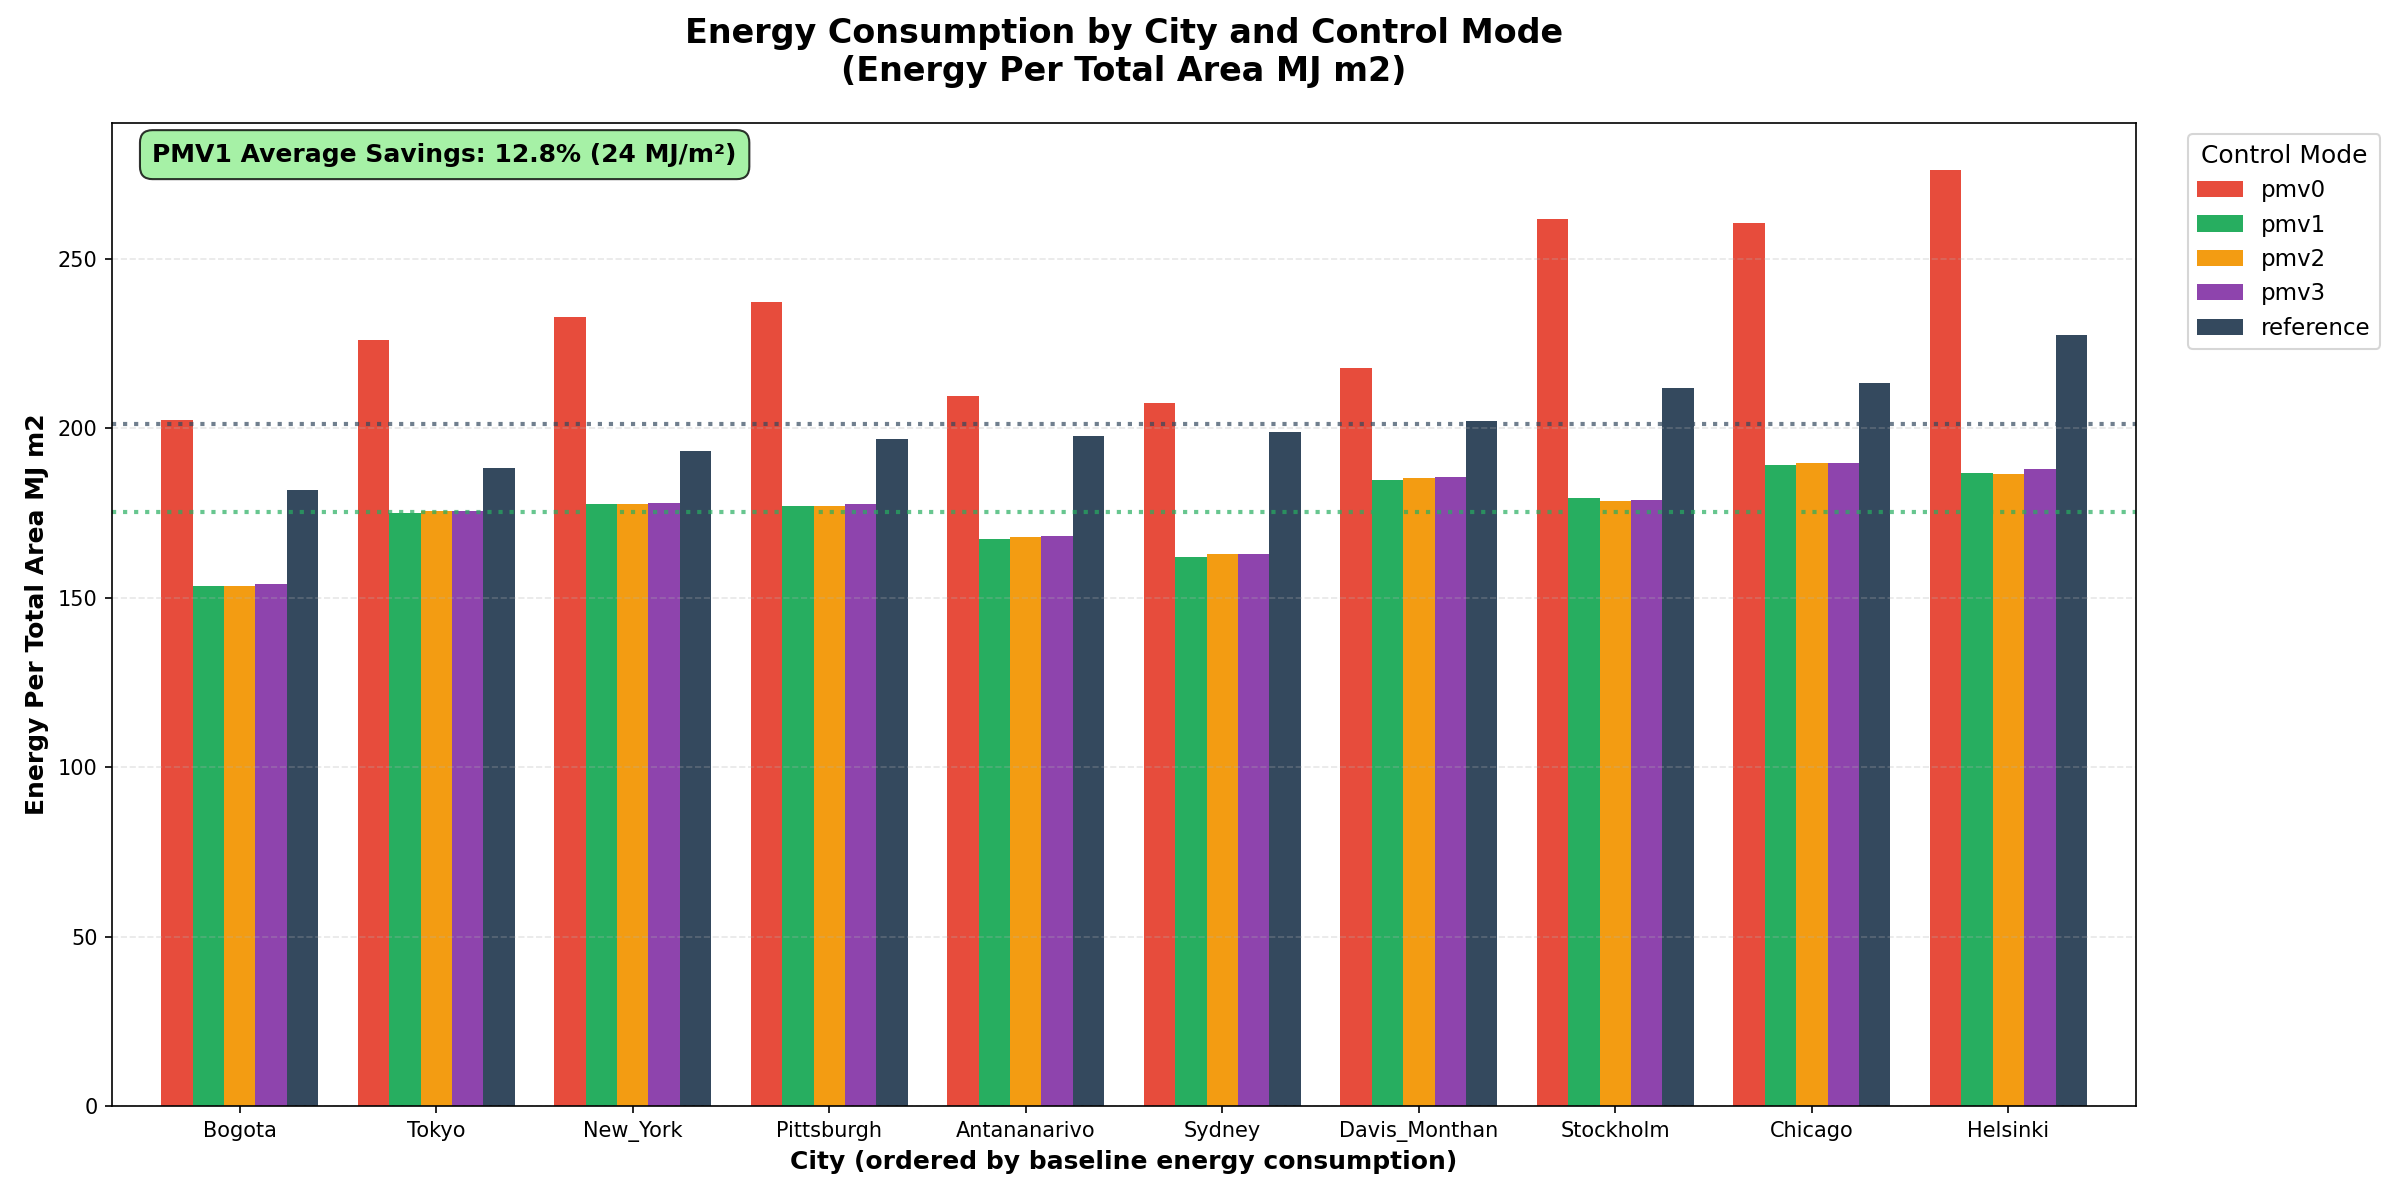
\includegraphics[width=0.95\linewidth]{figs/Energy_Per_Total_Area_MJ_m2_pmv.png}
    \caption{Energy per total area savings across all climates between reference state and all PMV-based control mode variations.}
    \label{fig:MJm2pmv}
\end{figure}

This can be better seen in Figure~\ref{fig:MJm2pmv}, where grid-search approach (\texttt{pmv1}, \texttt{pmv2}, \texttt{pmv3}) is broadly helpful and effective in achieving energy savings. These strategies consistently outperformed both the reference bang-bang control and the simplistic \texttt{pmv0} strategy. Optimized PMV-based control achieved consistent energy savings (averaging at around 12.75\% for PMV1), notably matching ML-based controls. This highlights the unexpected yet robust efficiency achievable by classical comfort models when systematically optimized.

The results clearly highlight that the grid-search approach (pmv1, pmv2, pmv3) is broadly helpful and effective in achieving energy savings. These strategies consistently outperformed both the reference bang-bang control and the simplistic pmv0 strategy. Notably, the three grid-search variants yielded remarkably similar energy savings within each city—typically varying by only one or two percentage points—suggesting that the underlying framework of PMV-based grid search with energy/comfort trade-offs is inherently robust. This convergence in performance indicates there is no single "one-solution-fits-all" strategy among pmv1, pmv2, and pmv3 that consistently yields superior energy results across all diverse climates. While all are effective, the specific parameters (weights, step sizes) explored in these variants might lead to different comfort experiences for occupants, which is not captured in this EUI data but would be a critical consideration for practical implementation. The choice among these similar-performing strategies might ultimately hinge on their differential impact on occupant comfort or other operational considerations beyond pure energy efficiency.

Optimized PMV controls consistently achieved significant (15–18.5\%) or moderate (7–11.5\%) energy savings across diverse climates, demonstrating robust performance independent of geographic and climatic variations. This highlights that grid-search optimization of classical comfort models effectively balances comfort and energy efficiency, rivaling sophisticated ML models.

\subsubsection{Observed Energy Savings with Grid‐Search PMV Optimization}
\label{sec:pmv_energy}

Figure~\ref{fig:stockholm-tokyo} illustrates how the \texttt{pmv1} grid‐search control exploits climatic differences to widen the neutral comfort band. In Stockholm’s cold‐continental summer, lower humidity allows indoor temperatures to reach 27–28\,$^\circ$C (a 5–7\,$^\circ$C expansion from the baseline) without violating PMV neutrality, effectively utilizing `free cooling' from economizer mode operation from June through September. Tokyo's humid-subtropical summer climate restricts this expansion to only 2–3\,$^\circ$C (25–26\,$^\circ$C) due to higher humidity levels that affect thermal comfort. The PMV1 algorithm inherently recognizes these psychrometric constraints and maintains setpoint extremes until indoor conditions approach the boundaries of the expanded comfort range (see Figure~\ref{fig:zoomed-tkst}), resulting in extended economizer mode operation and substantial annual energy reductions without compromising occupant comfort.

\begin{figure}[h!]
    \centering
    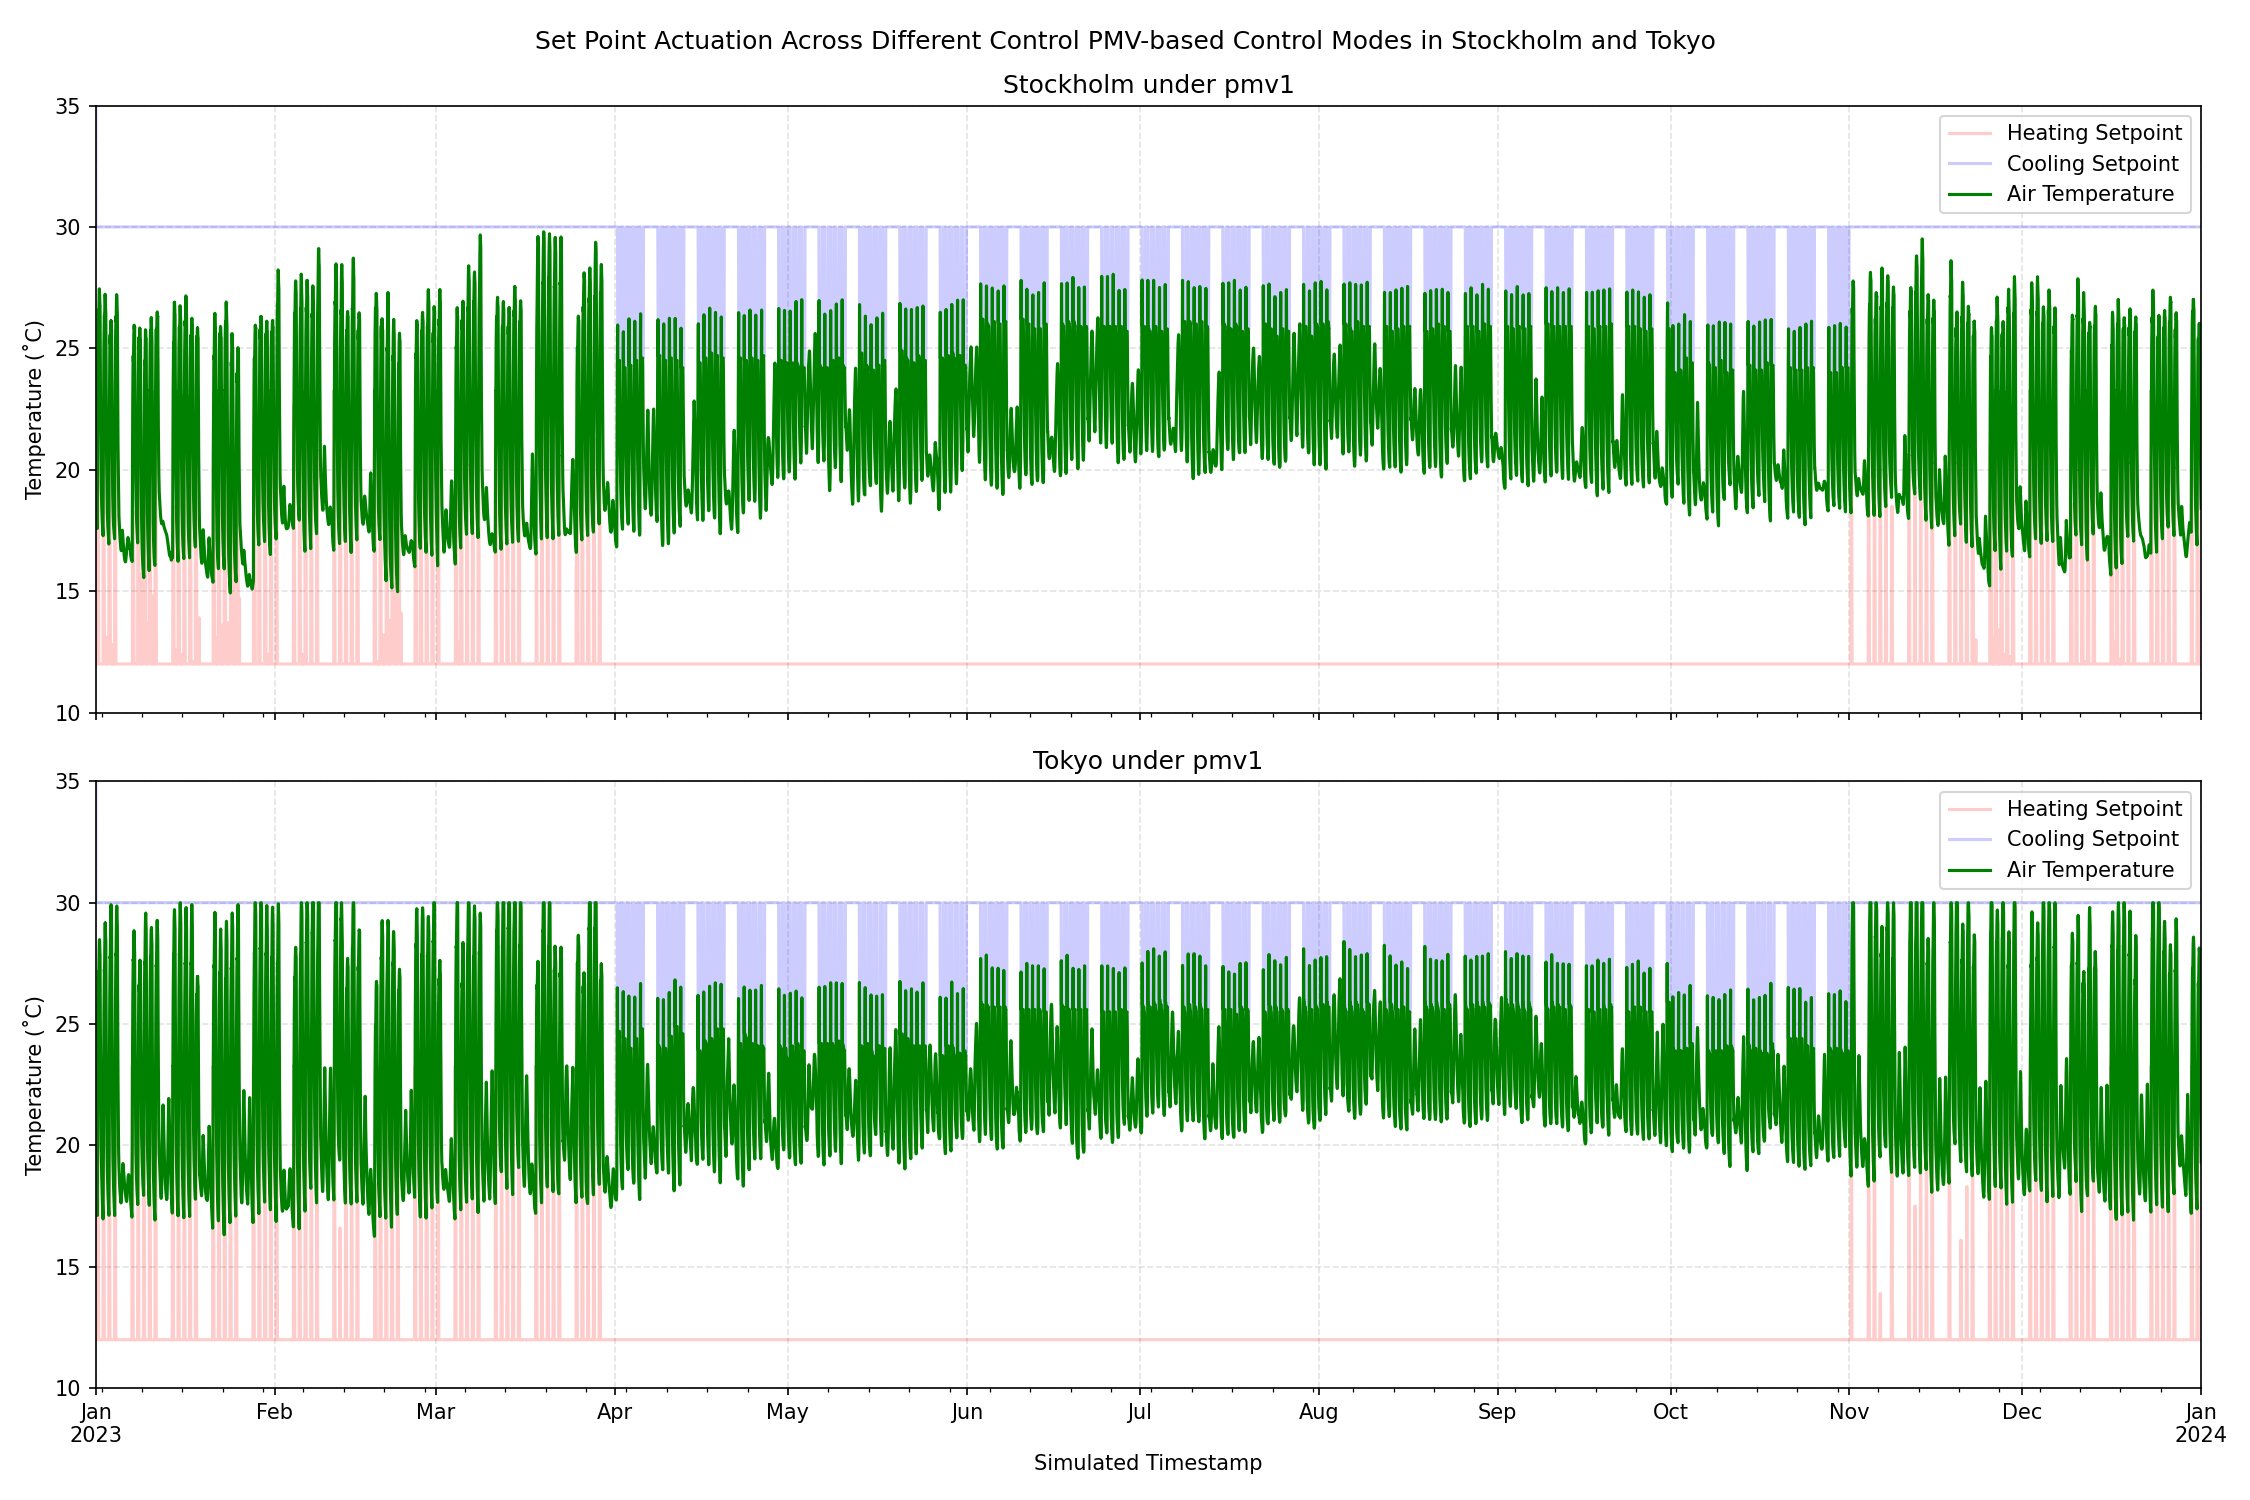
\includegraphics[width=0.95\linewidth]{figs/Stockholm_Tokyo.png}
    \caption{PMV1 control adaptation in contrasting climates: (a) Stockholm’s lower summer humidity permits indoor setpoints of 27–28\,$^\circ$C while maintaining PMV neutrality; (b) Tokyo’s higher humidity constrains summer setpoints to 25–26\,$^\circ$C.}
    \label{fig:stockholm-tokyo}
\end{figure}

\begin{figure}[h!]
    \centering
    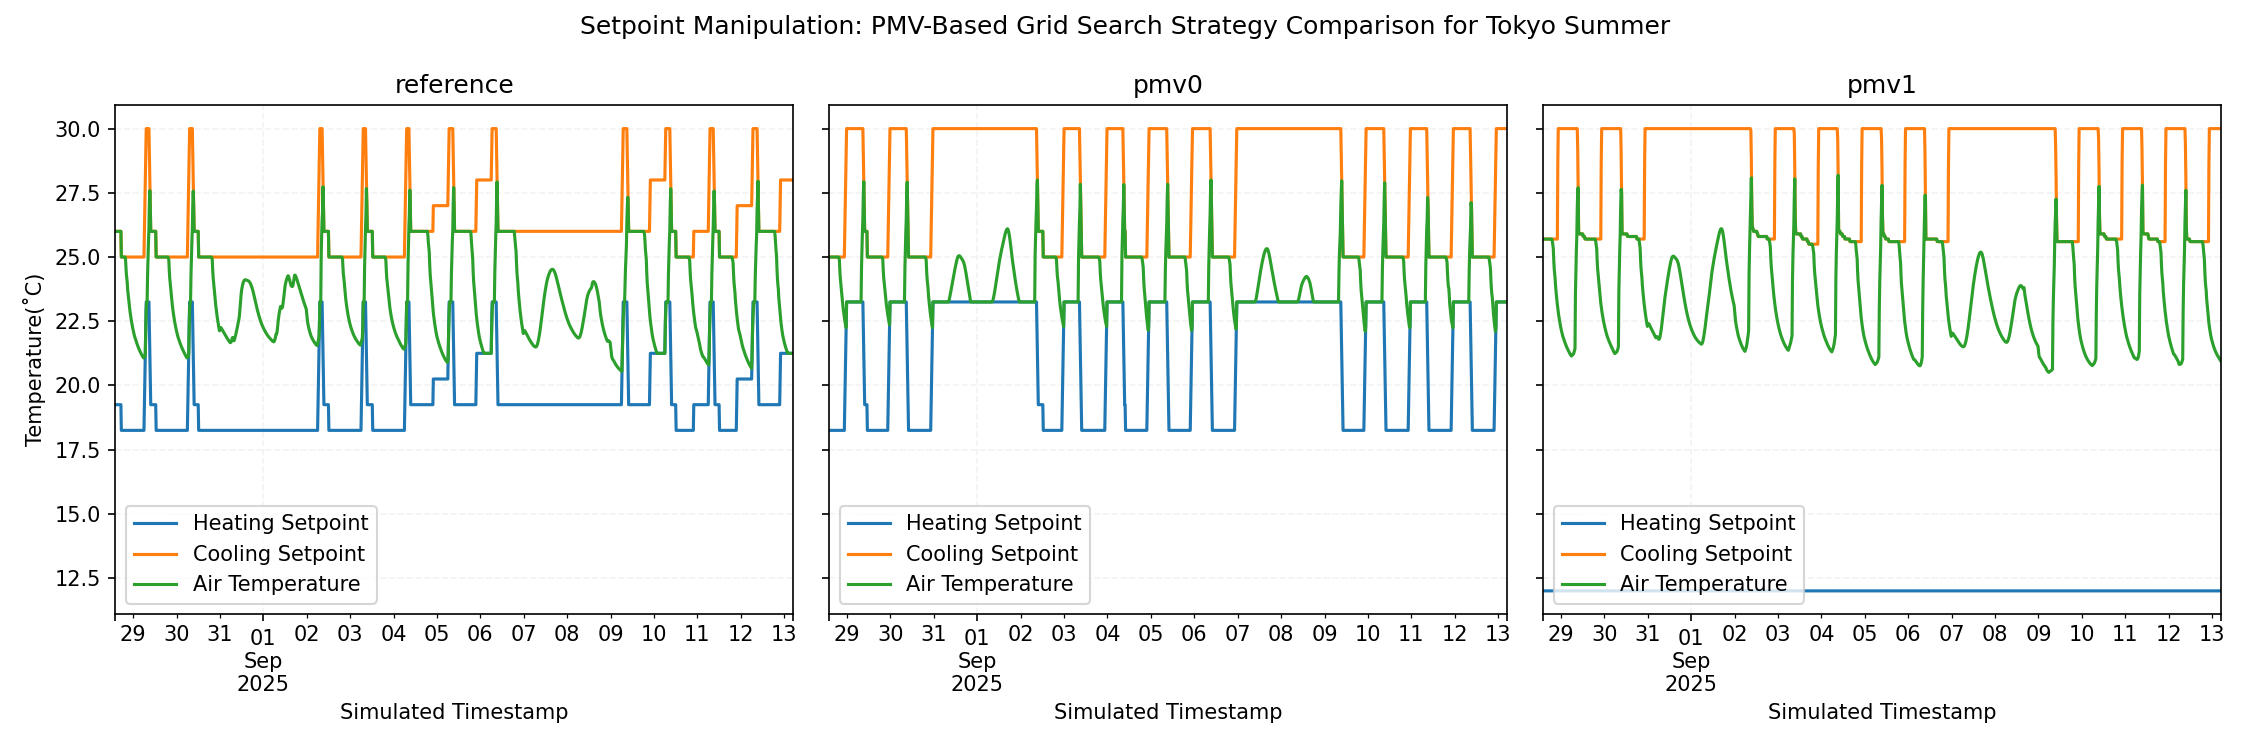
\includegraphics[width=0.75\linewidth]{figs/realcontrol_tk.png}
    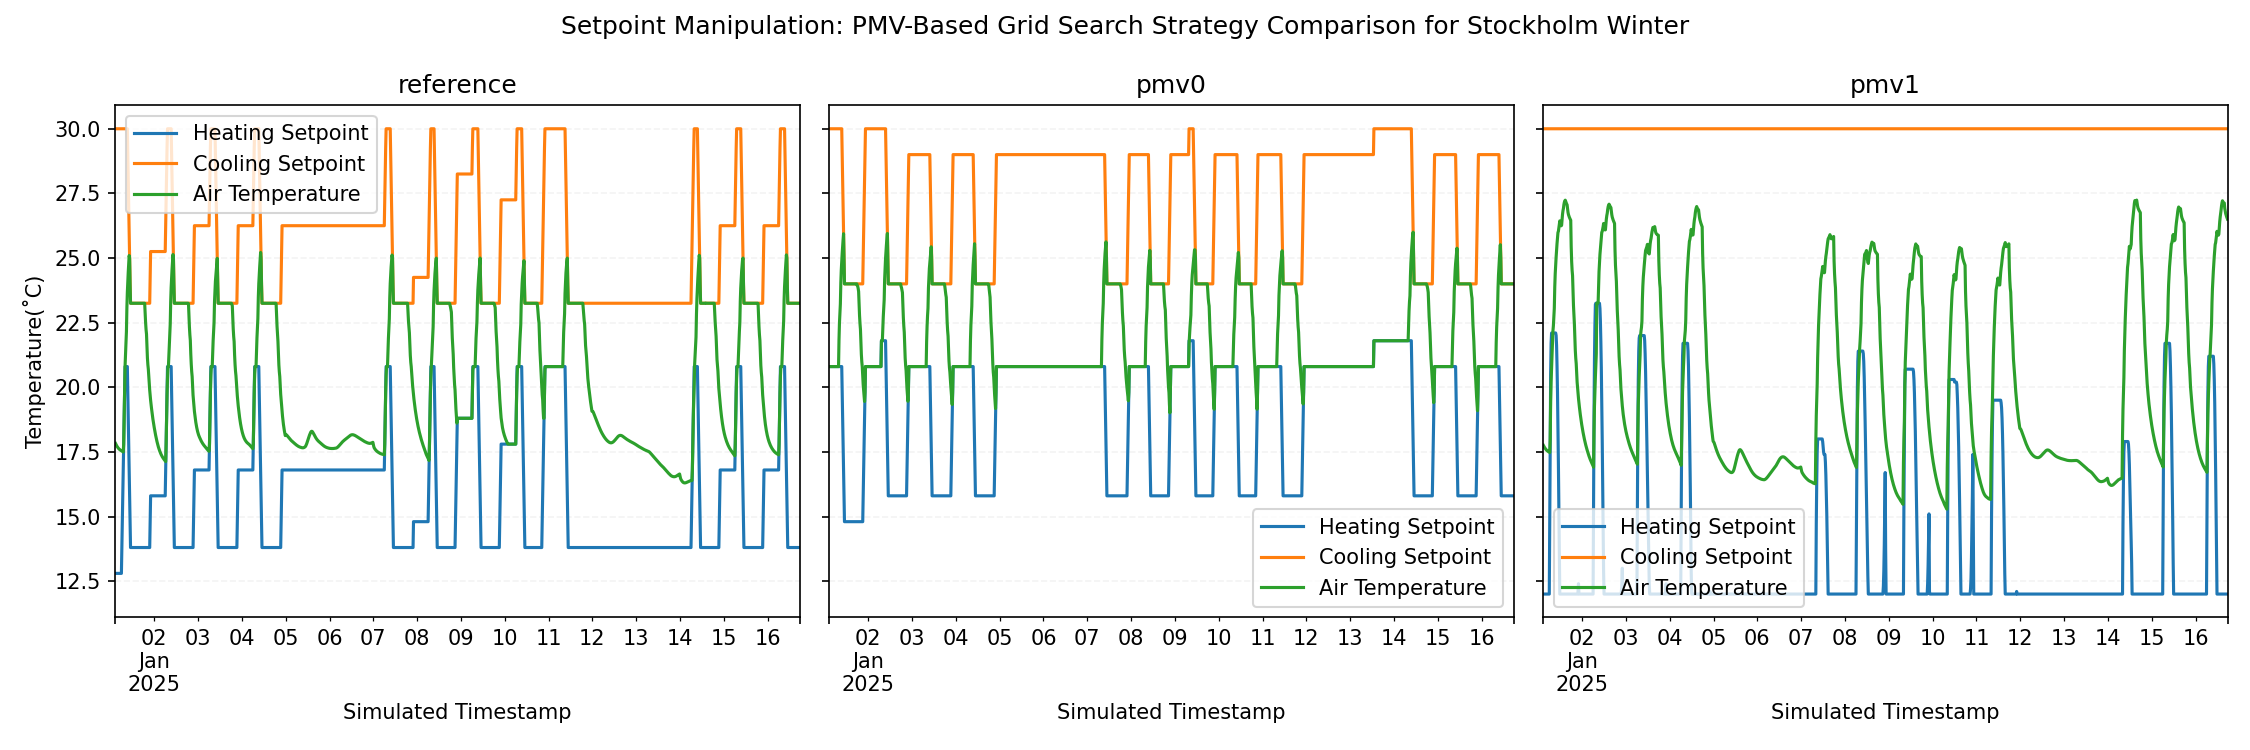
\includegraphics[width=0.75\linewidth]{figs/realcontrol_st.png}
    \caption{Detailed setpoint behavior under PMV1: (top) Tokyo summer holds cooling at the grid‐searched maximum until indoor temperature drifts outside the widened band; (bottom) Stockholm winter holds heating at the minimum as passive gains maintain comfort.}
    \label{fig:zoomed-tkst}
\end{figure}

\subsection{Control Strategy Comparison}
\label{sec:all_control_strategies}
As outlined in the methodology, we compared the seven different control scenarios across four different weather files within our selected IDF file, where we analyze their corresponding energy usage, thermal comfort status, and overall runtime. Figure~\ref{fig:runtime} presents the runtime comparison between the 7 control scenarios. As anticipated, the reference case is consistently the fastest, typically completing annual simulations in 15-20 seconds with no external components to communicate. PMV shows comparable performance at similar runtimes since it's also an analytical model using deterministic calculations. The machine learning models show significantly longer runtimes. LightGBM takes approximately 150-200 seconds per simulation—roughly 10 times slower than reference/PMV—due to model loading and prediction for anticipated occupant arrays. PINN-VAE demonstrates even longer runtimes at 600-900 seconds, as deep learning models require more computational overhead despite vectorized processing.

\begin{figure}[h!]
    \centering
    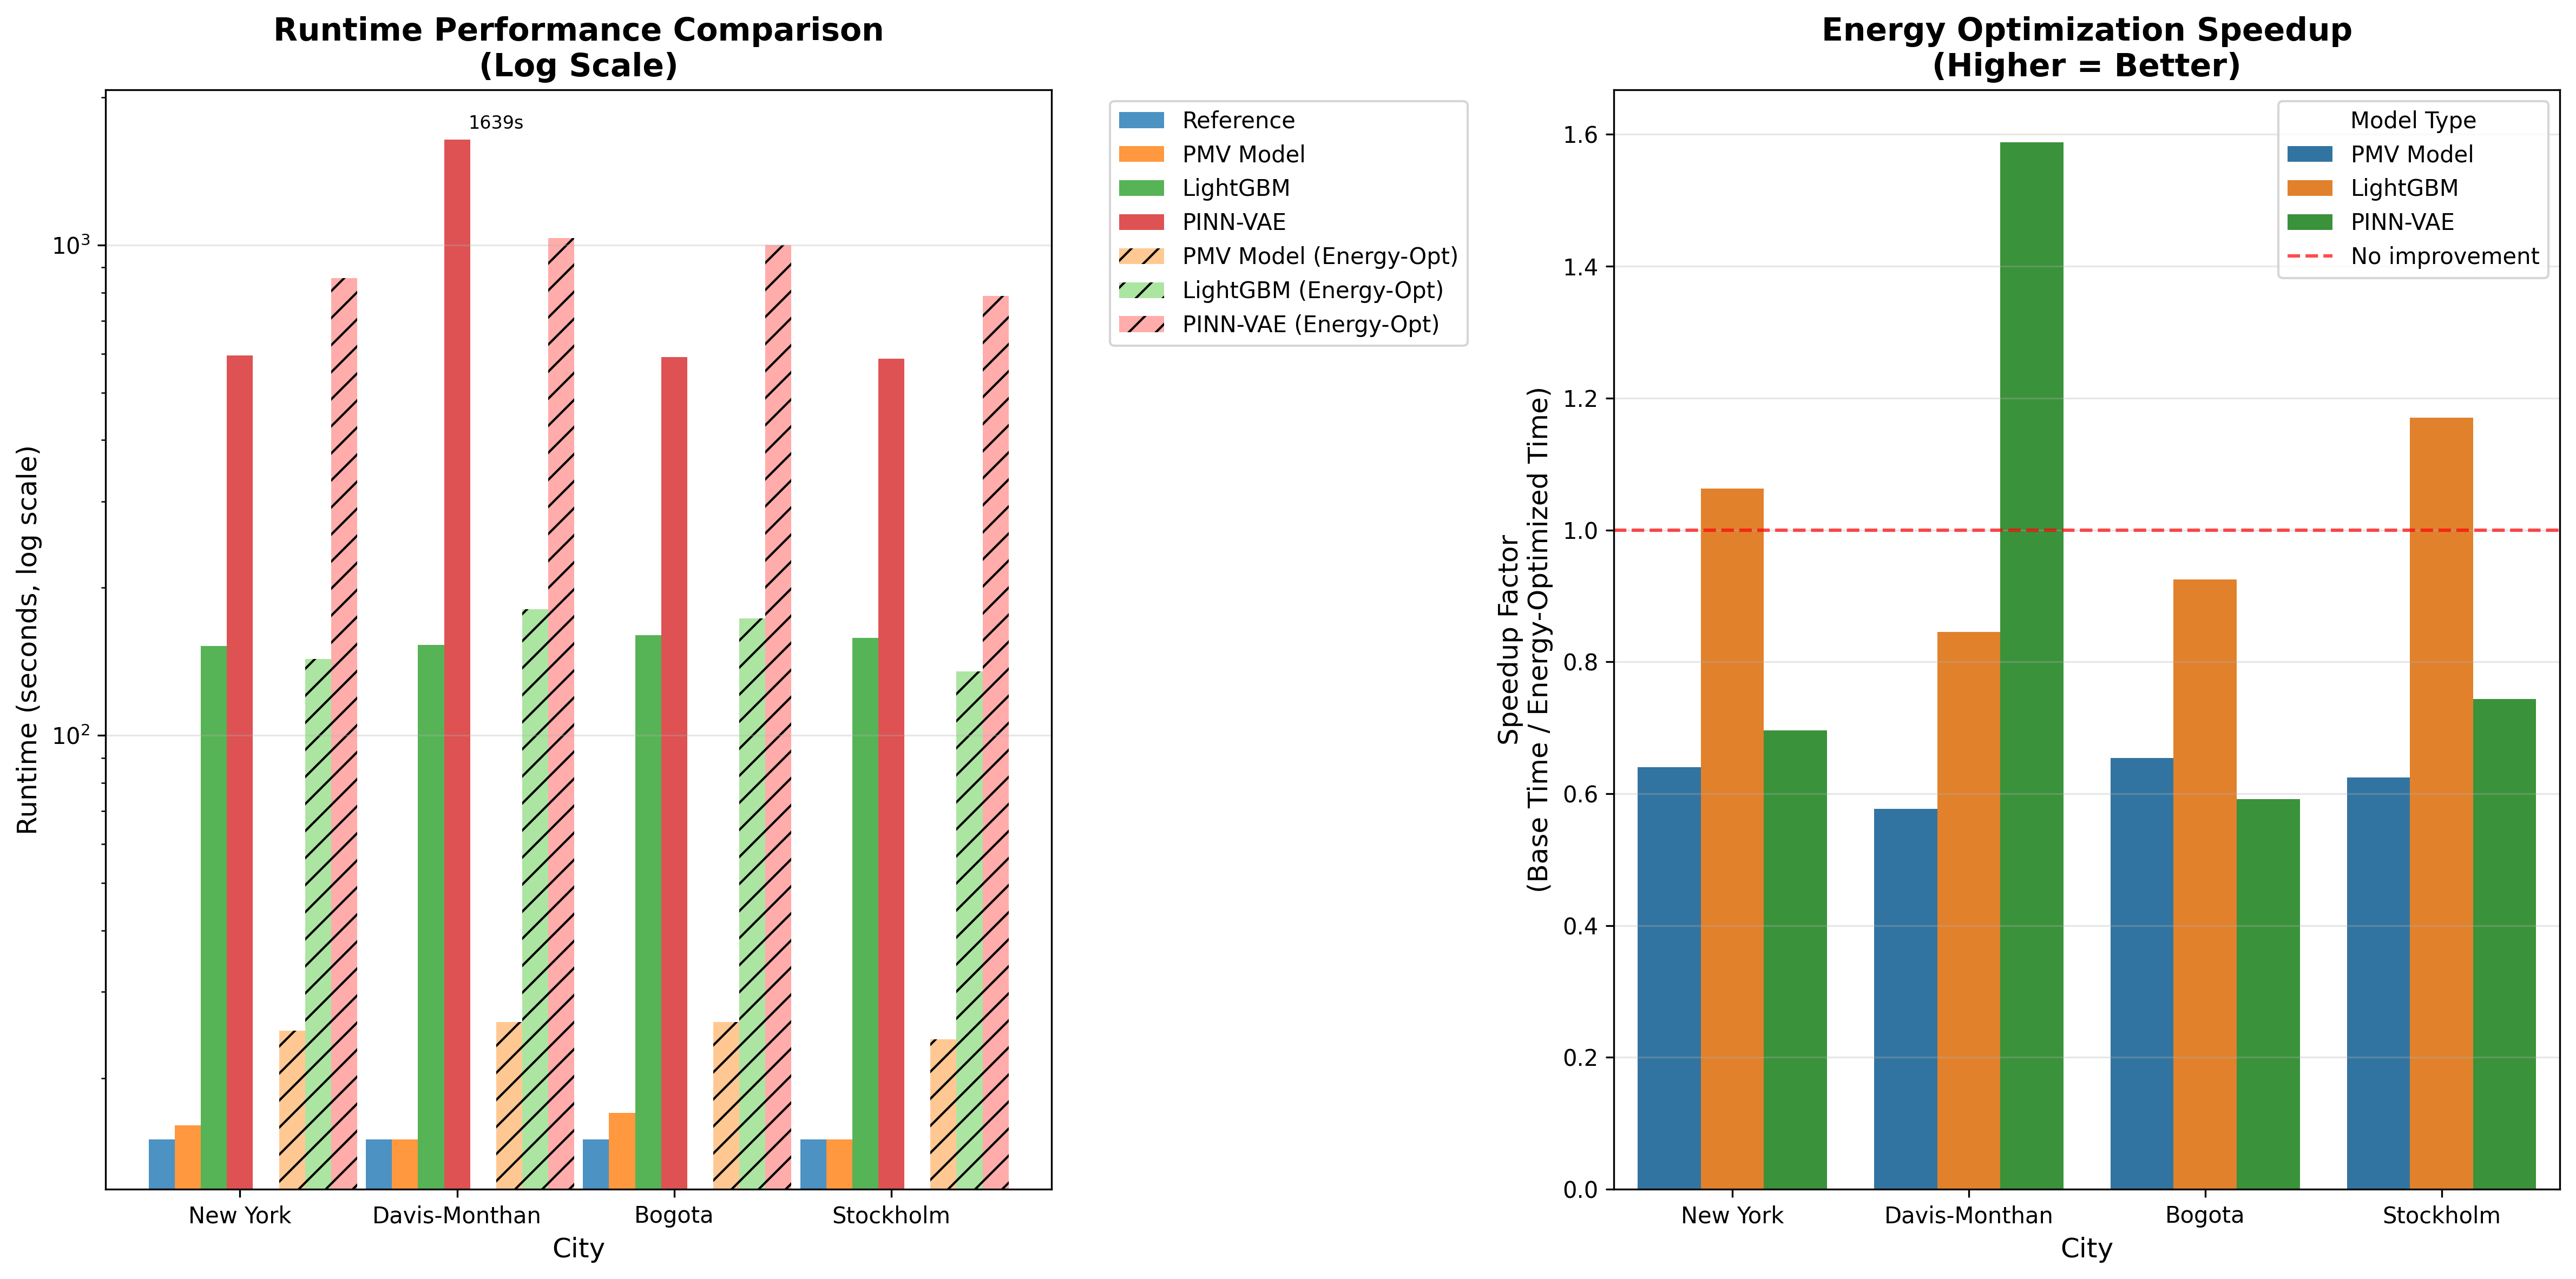
\includegraphics[width=0.75\linewidth]{figs/runtime.png}
    \caption{Runtime comparison between different thermal sensation prediction base models and computational time increase from implicit energy-saving $\Delta T$ grid search.}
    \label{fig:runtime}
\end{figure}

In contrast, the grid search optimization (`-o' variants) reveals interesting patterns: for PMV and LightGBM, the grid search approximately doubles runtime compared to their base versions, reflecting the computational cost of evaluating multiple temperature offset scenarios. However, PINN-VAE shows minimal runtime increase with optimization (comparing `pv' to `pv-o'), suggesting that model inference time dominates over the additional grid search computations. These runtime differences have important implications for real-time control applications, where the sub-200 second performance of optimized PMV and LightGBM remains practical, while PINN-VAE's 10-15 minute runtimes may limit its deployment to offline optimization scenarios.

\subsubsection{Energy Usage and Thermal Comfort Statistics}
\label{sec:energy_comfort_analysis}
This section analyzes the quantitative energy and comfort outcomes of each control strategy, examining total consumption, component-level breakdowns, and thermal comfort distributions.
We first examine the energy and comfort performance of each control strategy. Figure~\ref{fig:energy_ranking} presents the annual energy consumption ranking (1 = most efficient) for each control mode in Bogota, Davis‐Monthan, New York, and Stockholm. Across all four climates, the optimized grid‐search variants (\texttt{pmv-o}, \texttt{lightgbm-o}, \texttt{pv-o}) consistently occupy the top three positions, demonstrating robust, climate‐independent performance. In contrast, the “pure” modes (\texttt{pmv}, \texttt{lightgbm}, \texttt{pv}) occupy the lower ranks (5–7), despite sometimes achieving localized cooling or fan energy reductions. This discrepancy arises because unoptimized controllers frequently request setpoints beyond the 12 $^\circ$C–30 $^\circ$C limits, leading to actuator clipping and spurious energy savings in one end use that are more than offset by large energy penalties in another. The baseline \texttt{reference} (`bang–bang') control invariably sits in the middle (rank 4), underscoring that naïve comfort‐based inversions can underperform a simple hysteresis thermostat when actuator saturation is not considered.

\begin{figure}[h!]
    \centering
    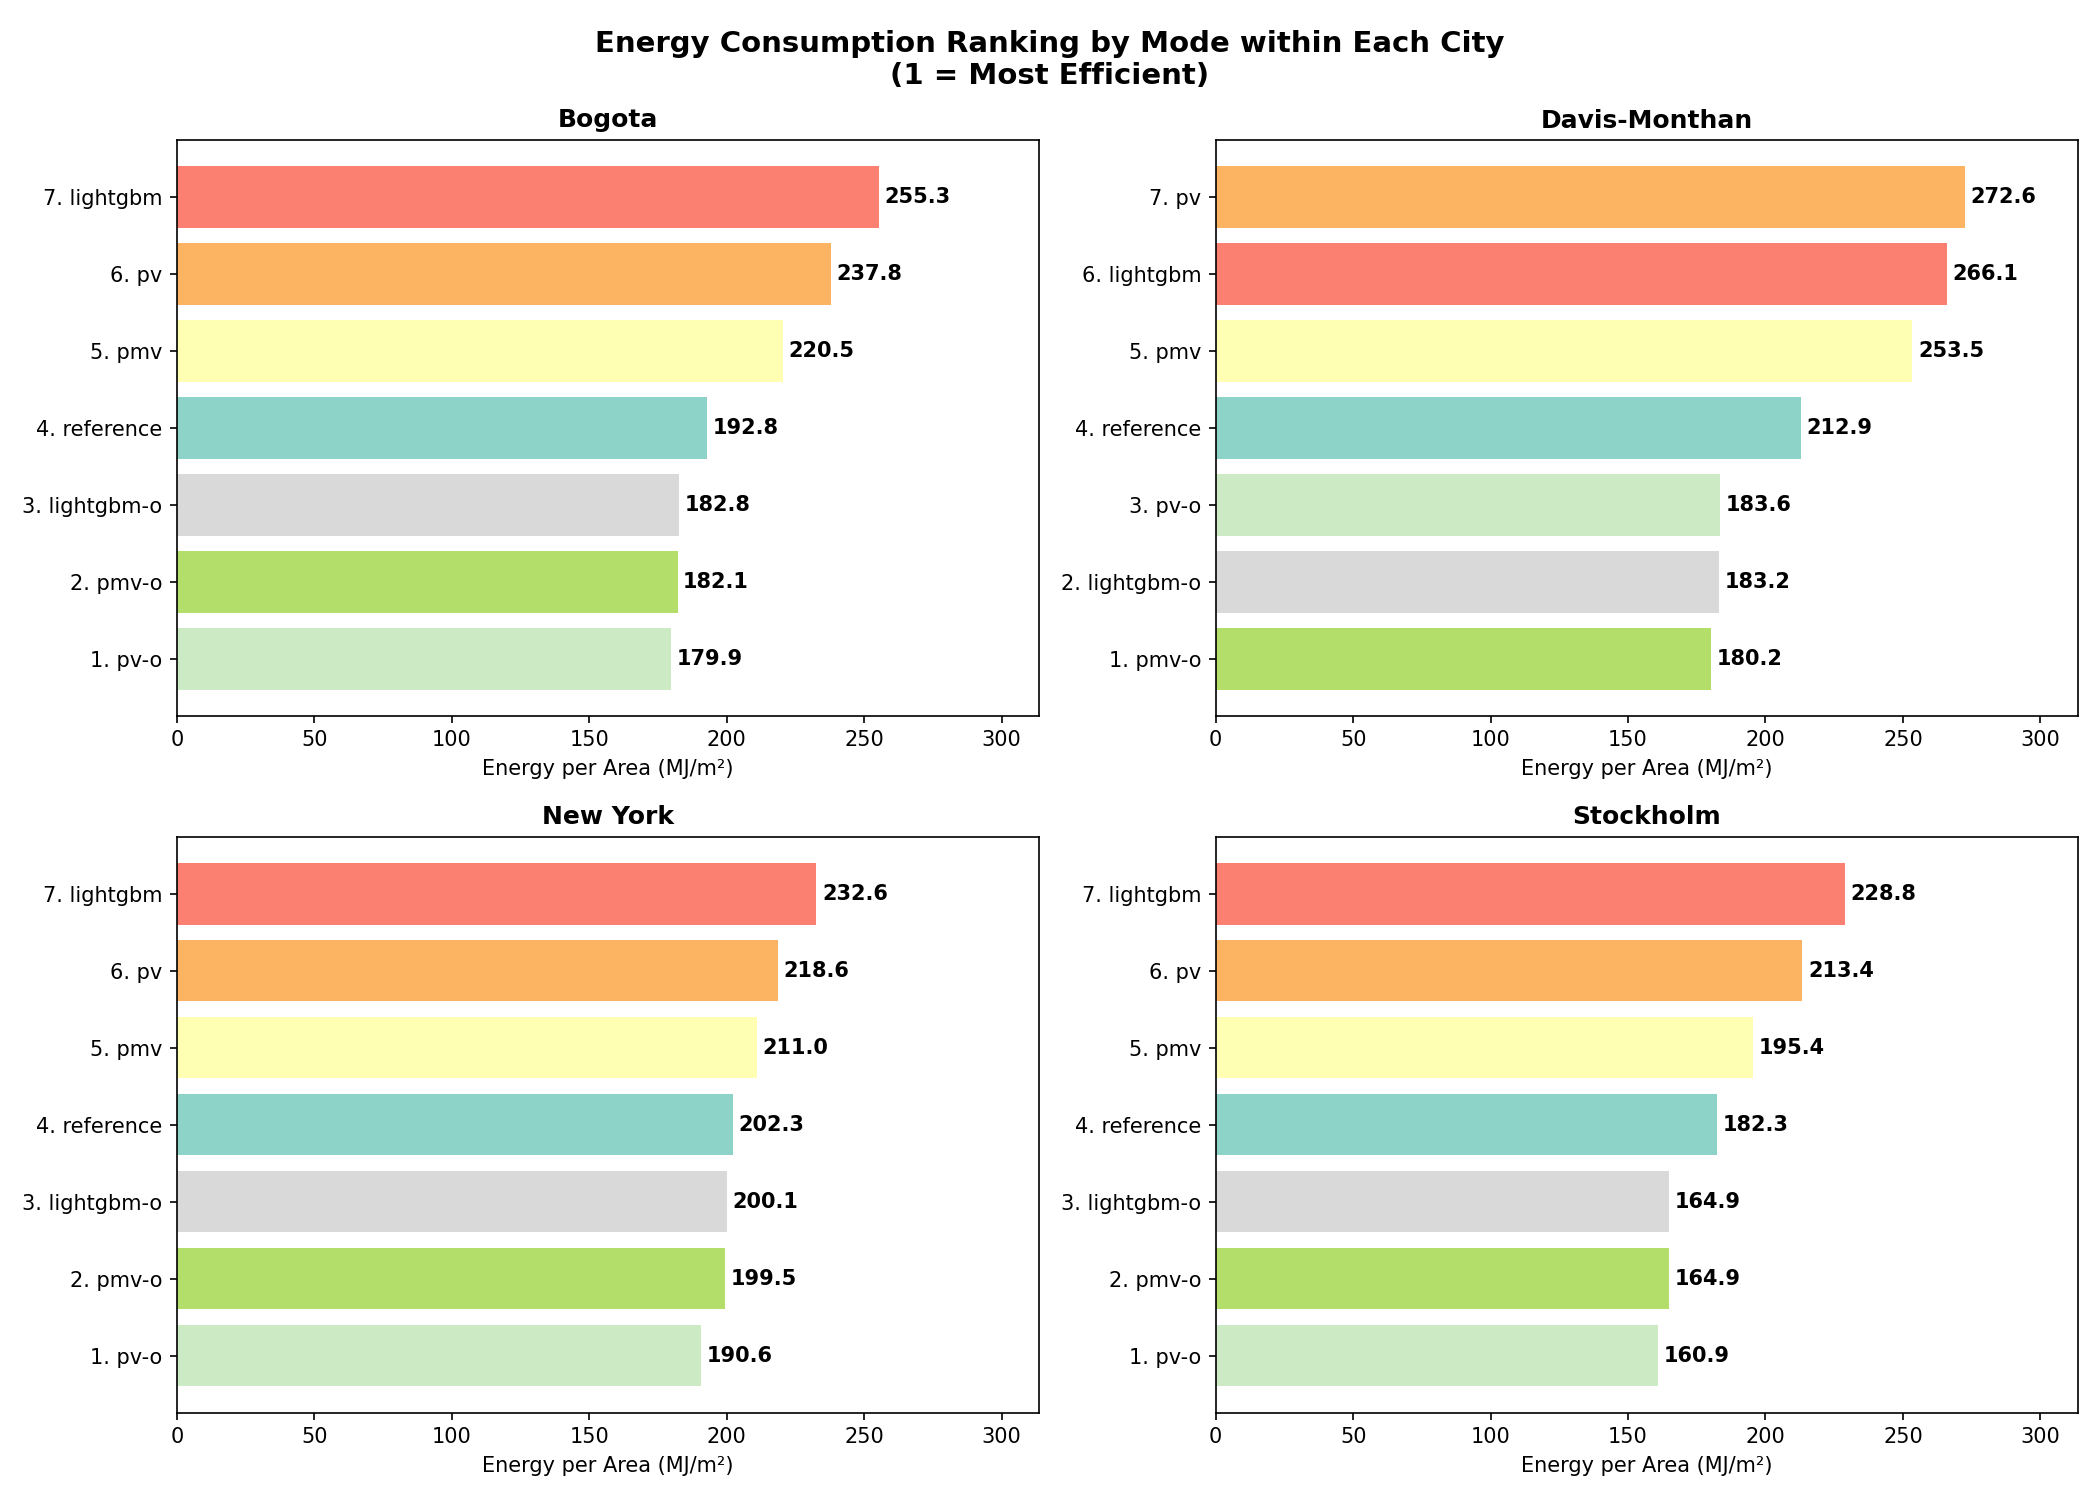
\includegraphics[width=\linewidth]{figs/energy_consumption_ranking_by_mode_within_each_city.png}
    \caption{Energy consumption ranking (1 = most efficient) for each control mode in four cities. Grid‐search variants (\texttt{pmv-o}, \texttt{lightgbm-o}, \texttt{pv-o}) occupy the top three ranks, while unoptimized “pure” modes (\texttt{pmv}, \texttt{pv}, \texttt{lightgbm}) lie at the bottom.}
    \label{fig:energy_ranking}
\end{figure}

Figure~\ref{fig:thermal_comfort} compares thermal comfort (Predicted Mean Vote, PMV) and indoor temperature distributions across all seven modes in the same four cities. The grid‐search variants maintain median PMV values tightly within the neutral band (–0.5 to +0.5) and exhibit markedly smaller interquartile ranges than the pure modes. For example, \texttt{pv-o} and \texttt{pmv-o} rarely exceed $\pm$0.5, indicating consistent comfort despite varying external conditions. By contrast, \texttt{lightgbm} and \texttt{pv} without optimization show bimodal PMV distributions, with frequent excursions above +1.0 or below –1.0, reflecting repeated setpoint clipping at 12$^\circ$C or 30$^\circ$C. These clipping‐induced comfort violations correspond to the oscillatory indoor temperature patterns visible in the lower panel: the pure ML/PV modes force indoor air to swing between the extremes of 12$^\circ$C and 30$^\circ$C, whereas grid‐search controllers keep most of their temperatures in the 22–26$^\circ$C range. This stabilization of indoor conditions not only preserves occupant comfort but also eliminates the energy wasted on cycling between extremes.

\begin{figure}[h!]
    \centering
    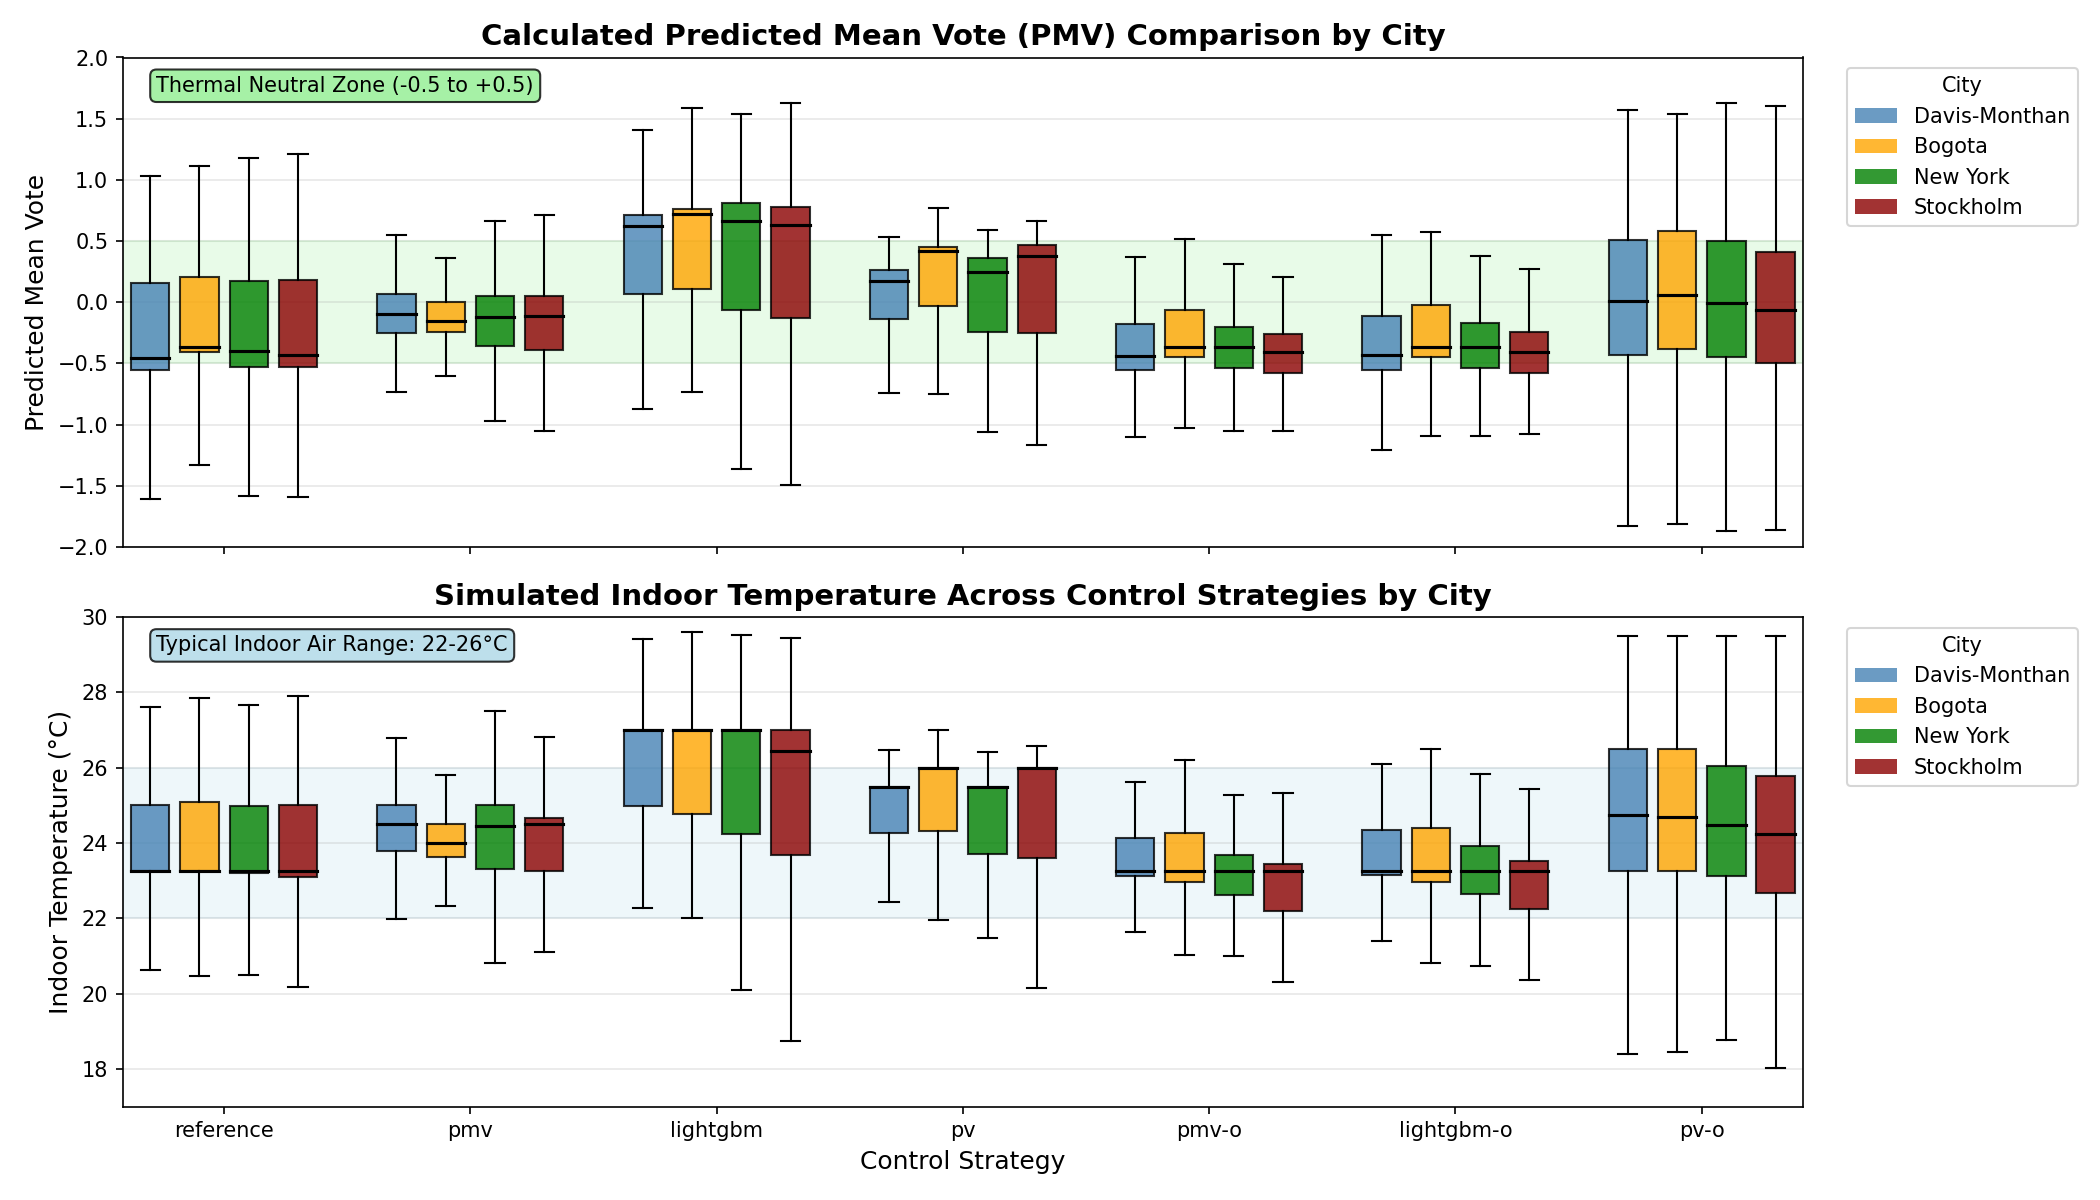
\includegraphics[width=\linewidth]{figs/thermal_comfort_comparison_improved.png}
    \caption{Top: PMV distributions by control mode and city (green shading = comfort zone, $\pm$0.5). Bottom: Indoor temperature distributions (blue shading = typical comfort range, 22–26$^\circ$C). Grid‐search variants exhibit tighter comfort control and avoid clipping‐induced extremes.}
    \label{fig:thermal_comfort}
\end{figure}

Figure~\ref{fig:component_savings} breaks down energy savings (relative to \texttt{reference}) into heating, cooling, and fan components for each city. The grid‐search PMV variant (\texttt{pmv-o}) achieves the largest heating reductions—up to +91\% in Bogota and +79\% in Davis—by tolerating expanded neutral temperature bands in summer and leveraging passive gains in winter. Although \texttt{pmv-o} incurs small negative cooling savings in colder climates (e.g., –16\% in Stockholm), the net effect is still a substantial reduction in overall HVAC energy. Similarly, \texttt{lightgbm-o} and \texttt{pv-o} realize significant heating savings (+58\% to +75\%) with modest cooling trade‐offs. In contrast, the unoptimized \texttt{lightgbm} and \texttt{pv} modes display large negative heating “savings”—for instance, –889\% in Davis and –295\% in New York—because they remain pinned at 12$^\circ$C during extremes and then must repeatedly reheat, creating enormous energy penalties. Their apparent cooling or fan energy gains are insufficient to offset these heating losses, confirming that actuator clipping can produce misleading component‐level metrics.

\begin{figure}[h!]
    \centering
    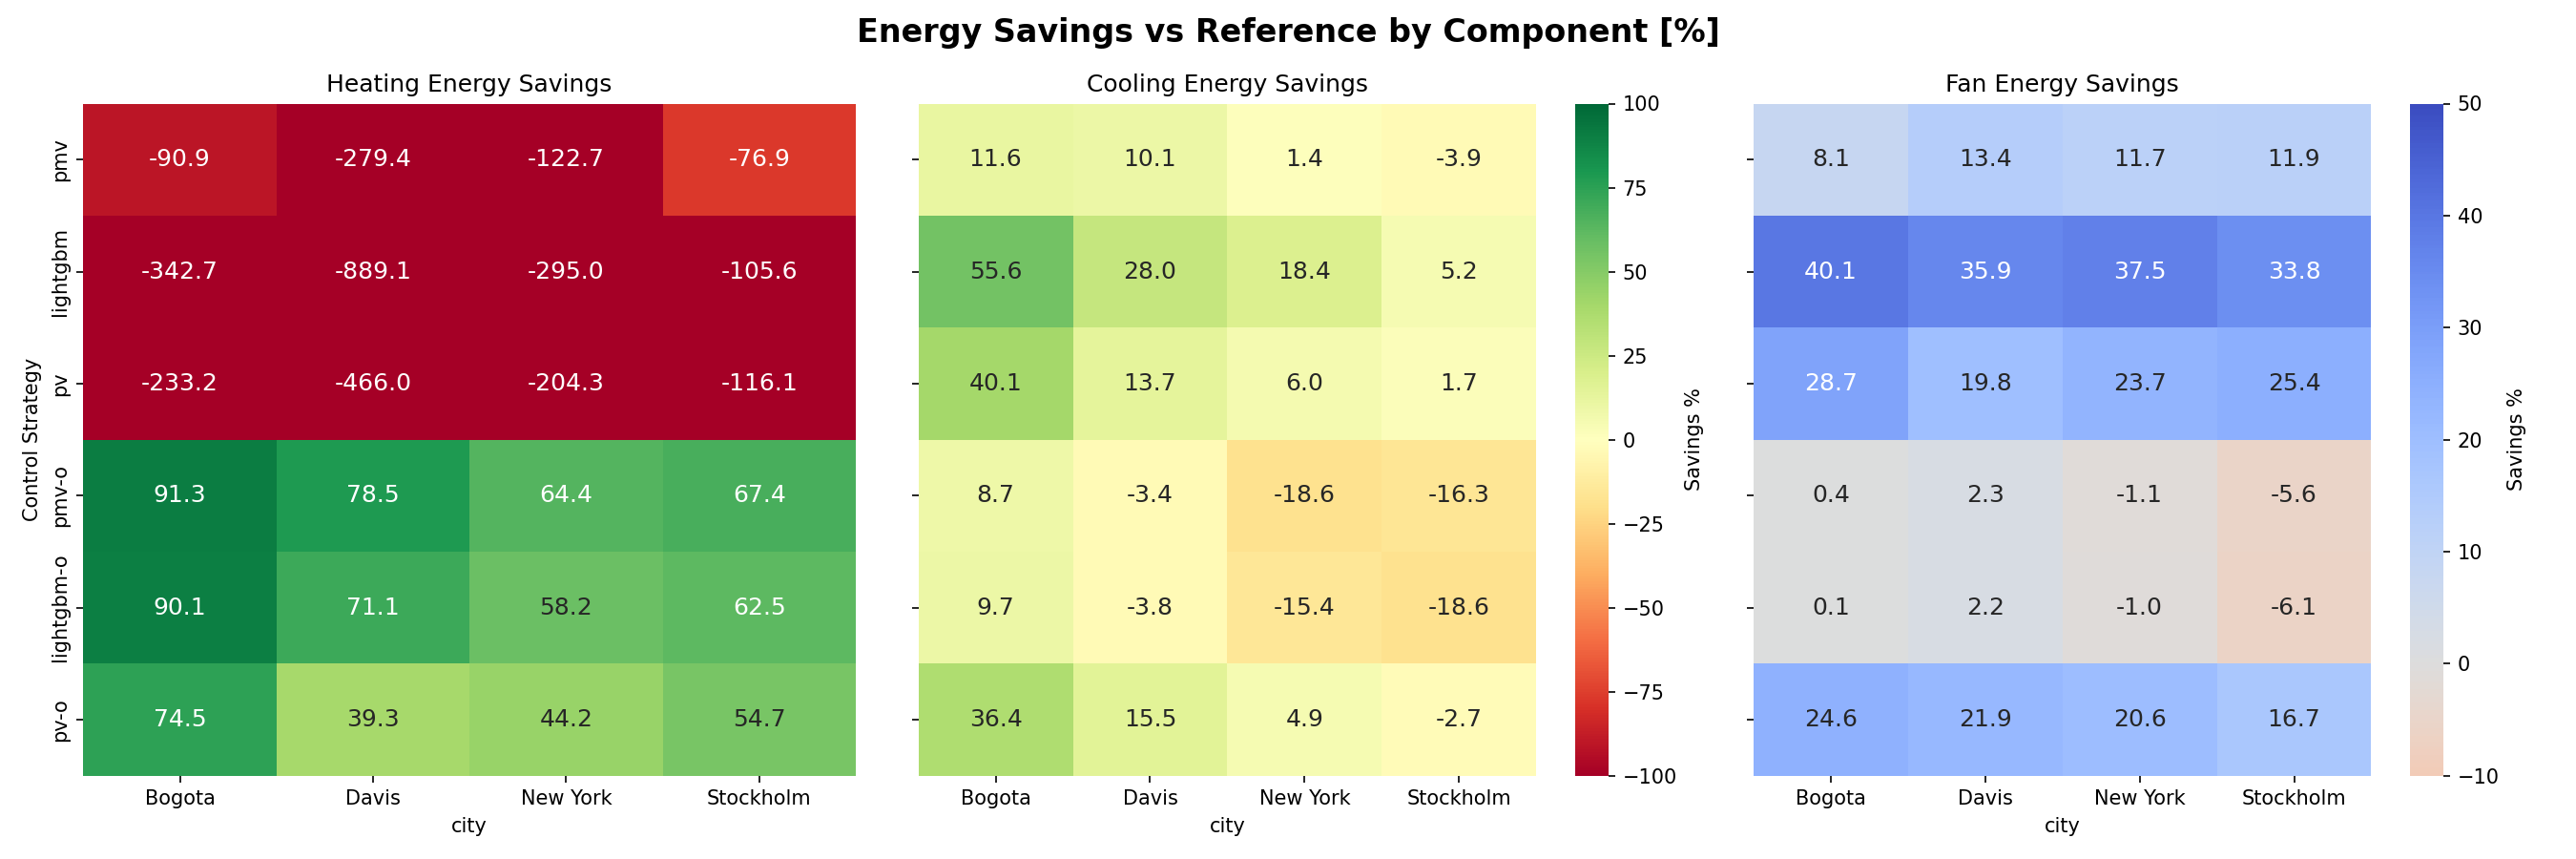
\includegraphics[width=\linewidth]{figs/saving_end_pct.png}
    \caption{Component‐level energy savings (\%) relative to \texttt{reference}, by city and control mode. Positive values indicate reduced consumption. Grid‐search variants (\texttt{pmv-o}, \texttt{lightgbm-o}, \texttt{pv-o}) achieve large heating savings with minor cooling/fan trade‐offs, while pure modes incur large heating penalties due to clipping.}
    \label{fig:component_savings}
\end{figure}

When aggregated into total HVAC energy savings (Figure~\ref{fig:hvac_savings}), grid‐search variants consistently deliver substantial net reductions—from 90\% in Bogota to 62\% in Stockholm—highlighting the method’s ability to achieve “win–win” outcomes: maintaining neutral PMV and stable indoor temperatures while dramatically lowering energy use. In contrast, pure \texttt{lightgbm} and \texttt{pv} modes produce negative net savings across all climates (e.g., –466\% in Davis, –204\% in New York), reflecting their pathological reliance on setpoints clipped to extremes. The \texttt{reference} controller (0\% savings by definition) outperforms unoptimized pure modes in some climates, underscoring that a simplistic hysteresis thermostat can surpass naïve comfort‐driven logic when actuator saturation is unresolved.

\begin{figure}[h!]
    \centering
    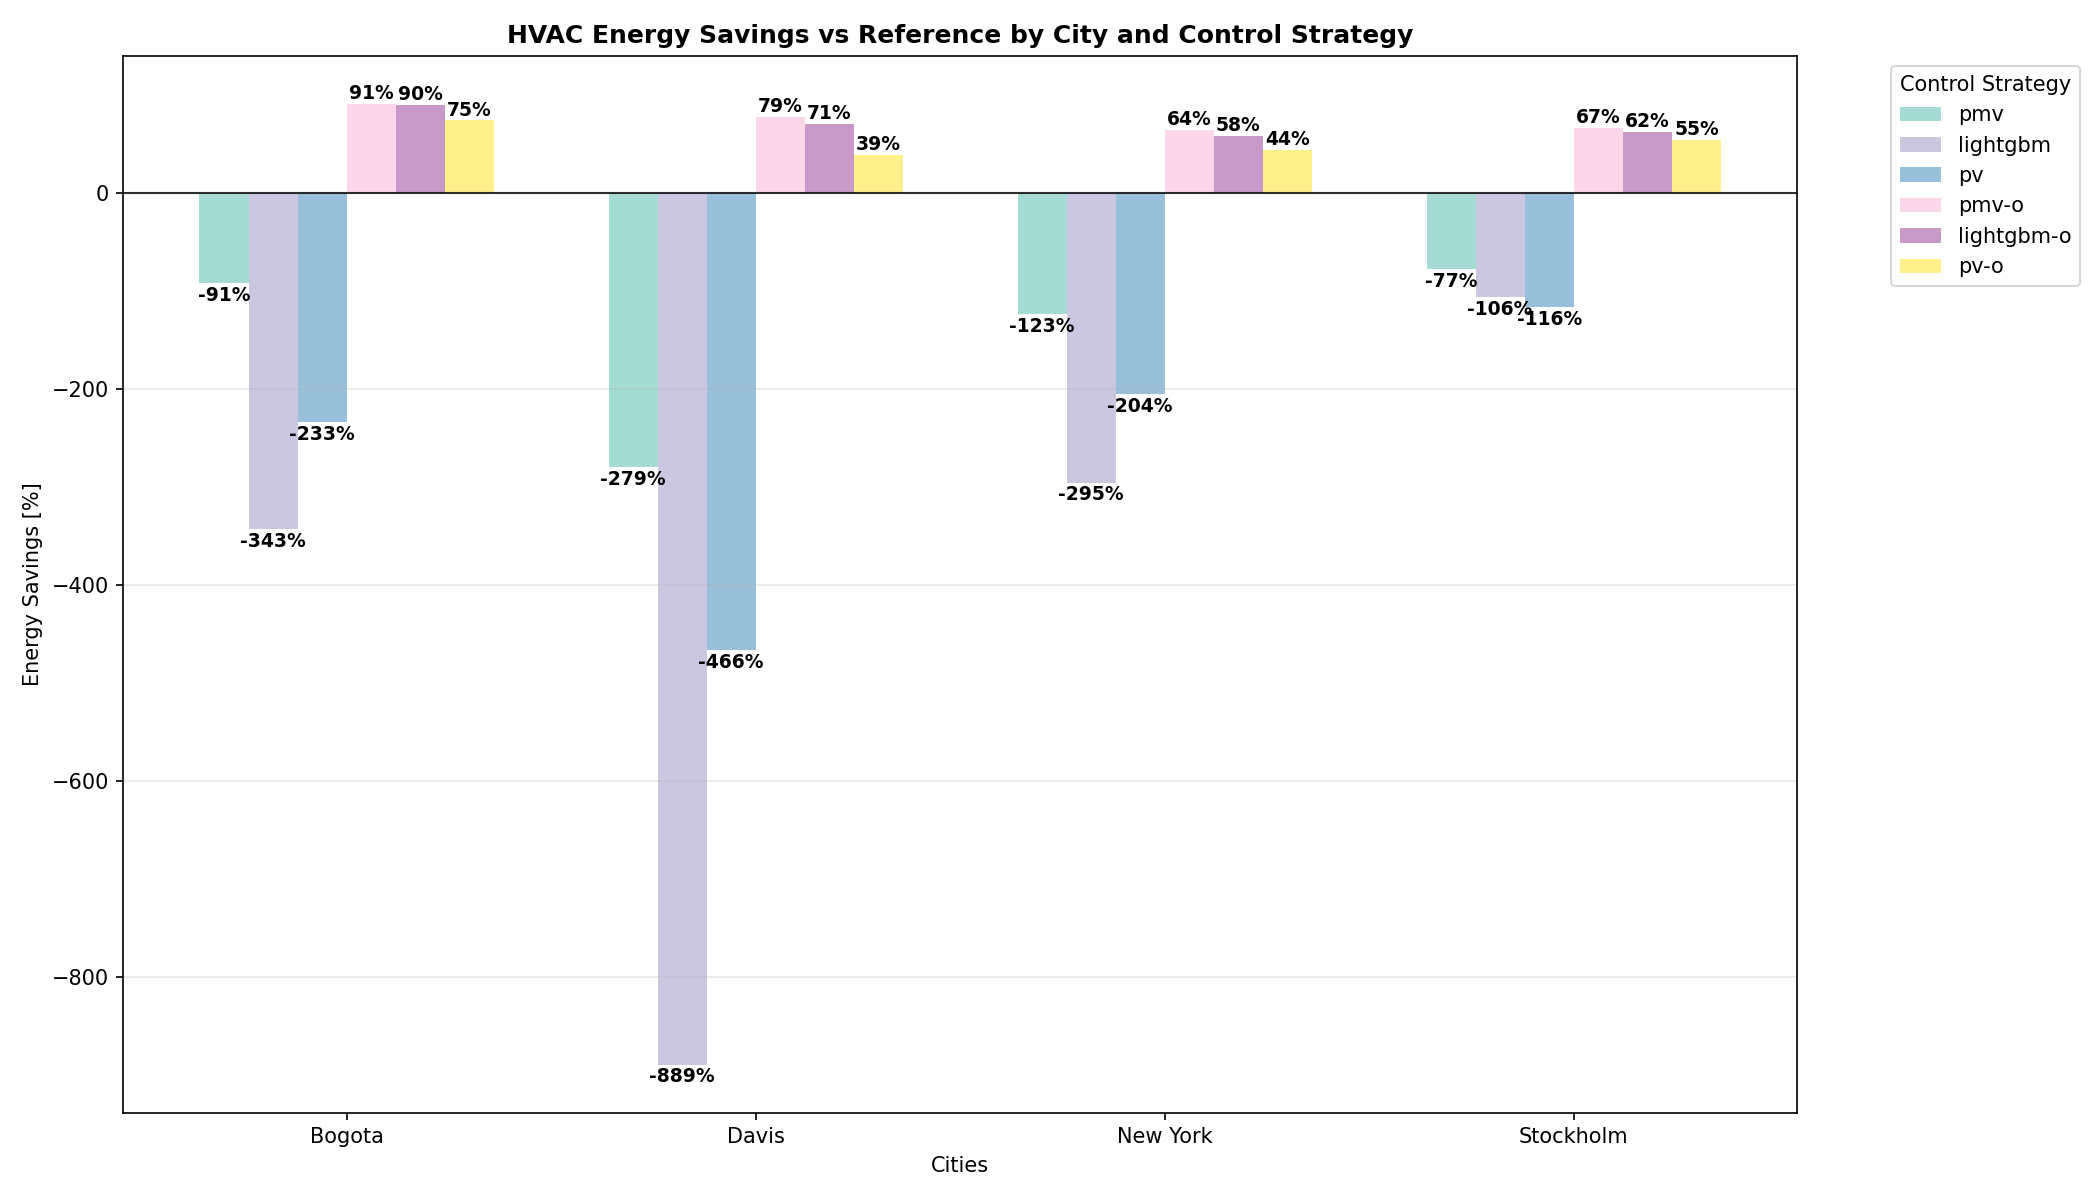
\includegraphics[width=\linewidth]{figs/savings_r.png}
    \caption{Total HVAC energy savings (\%) relative to \texttt{reference} across four cities. Grid‐search variants (\texttt{pmv-o}, \texttt{lightgbm-o}, \texttt{pv-o}) yield 62\%–90\% savings; unoptimized modes incur large negative savings due to actuator clipping.}
    \label{fig:hvac_savings}
\end{figure}


\subsubsection{Performance Hierarchy and Climate Consistency Analysis}
\label{sec:performance_hierarchy}
Having established the performance metrics, we now examine how these rankings remain consistent across diverse climates. 
As shown in Figure~\ref{fig:energy_ranking}, annual energy consumption (MJ/m²) for each control mode in Bogota, Davis‐Monthan, New York, and Stockholm (1 = most efficient) are plotted and ranked accordingly. Across all four climates, the optimized grid‐search variants (\texttt{pv-o}, \texttt{pmv-o}, \texttt{lightgbm-o}) occupy the top three positions, with \texttt{pv-o} and \texttt{pmv-o} typically tied for first or second. The baseline \texttt{reference} control consistently falls in the middle (rank 4), while the unoptimized “pure” modes (\texttt{pmv}, \texttt{pv}, \texttt{lightgbm}) occupy ranks 5–7, reflecting their inability to avoid actuator saturation.

While the previous section showed absolute performance differences, here we observe that climate-specific nuances appear primarily among the mid-rank and bottom modes, with top performers maintaining their advantage regardless of location. In Bogota and New York, \texttt{lightgbm-o} edges out \texttt{pmv-o} by a small margin, whereas in Davis‐Monthan and Stockholm, \texttt{pmv-o} ties or slightly outperforms \texttt{pv-o}. Among the unoptimized controllers, \texttt{pmv} often ranks lower in cold climates (Stockholm) but improves modestly in mixed or hot climates (Bogota, Davis‐Monthan). Similarly, \texttt{lightgbm} and \texttt{pv} without grid optimization display high variability—\texttt{lightgbm} fares better in New York but poorly in Davis‐Monthan, while \texttt{pv} consistently remains mid‐tier. Overall, the grid‐search optimization engenders both superior and more climate‐robust performance, demonstrating that a properly tuned analytical or ML‐based method consistently outperforms unoptimized strategies across diverse thermal conditions.


\subsubsection{Actuator Saturation Analysis}
\label{sec:actuator_saturation_results}
Our co-simulation methodology enables direct observation of actuator saturation behavior—a critical deployment challenge that pure comfort prediction research often overlooks. This phenomenon occurs when a controller's requested heating setpoint falls below the hard minimum ($12\,^\circ\mathrm{C}$) or its requested cooling setpoint exceeds the hard maximum ($30\,^\circ\mathrm{C}$). 
EnergyPlus (via Sinergym) then clips the setpoint to that boundary; further commands in the same direction have no effect. Table~\ref{tab:saturation_rates} demonstrates our framework's capability to quantify this saturation behavior, reporting the percentage of occupied hours during which each controller was clipped to 12 $\degree C$ or 30 $\degree C$ under both original and boundary-optimized implementations.

\begin{table}[!]
  \centering
  \caption{Percentage of occupied hours clipped to actuator bounds, before vs.\ after boundary optimization.}
  \label{tab:saturation_rates}
  \resizebox{\textwidth}{!}{
  \begin{tabular}{l|rrrrrr}
    \toprule
    \multirow{2}{*}{Controller Mode} & \multicolumn{3}{c}{Before} & \multicolumn{3}{c}{After} \\
    \cmidrule(lr){2-4} \cmidrule(lr){5-7}
    & \% @ 12~$^\circ$C & \% @ 30~$^\circ$C & \% Total Clipped
    & \% @ 12~$^\circ$C & \% @ 30~$^\circ$C & \% Total Clipped \\
    \midrule
    reference              & $0.00\%$ & $2.84\%$ & $2.84\%$ & $0.00\%$ & $2.85\%$ & $2.85\%$ \\
    PMV (pure)             & $0.00\%$ & $13.99\%$ & $13.99\%$ & $0.00\%$ & $0.10\%$ & $0.10\%$ \\
    LightGBM (pure)        & $4.52\%$ & $7.95\%$ & $7.95\%$ & $0.00\%$ & $4.52\%$ & $4.52\%$ \\
    PV (pure)              & $0.00\%$ & $0.39\%$ & $0.39\%$ & $0.00\%$ & $0.12\%$ & $0.12\%$ \\
    PMV-o (grid-search)    & $0.02\%$ & $66.95\%$ & $66.95\%$ & $0.00\%$ & $32.70\%$ & $32.70\%$ \\
    LightGBM-o (grid-search)& $0.00\%$ & $73.82\%$ & $73.82\%$ & $0.00\%$ & $32.70\%$ & $32.70\%$ \\
    PV-o (grid-search)     & $0.14\%$ & $67.76\%$ & $67.76\%$ & $0.00\%$ & $33.45\%$ & $33.45\%$ \\
    \bottomrule
  \end{tabular}
  }
\end{table}

Examining results from Table~\ref{tab:saturation_rates}, we could quickly come to the following key observations:
\begin{itemize}
  \item \textbf{Heating‐side saturation is eliminated after boundary optimization.} All controllers show $0.00\%$ clipped at $12\,^\circ\mathrm{C}$ in the ``After'' columns, confirming that the $\pm2\,^\circ\mathrm{C}$ grid around the interior reset prevents any candidate from falling below $12\,^\circ\mathrm{C}$.  
  \item \textbf{Cooling‐side saturation remains substantial.}  Even after boundary optimization, PMV‐o, LightGBM‐o, and PV‐o clip at $30\,^\circ\mathrm{C}$ approximately one‐third of occupied hours (32.70–33.45\%). This indicates that under hot conditions, all $\Delta T$ candidates eventually hit the hard ceiling, and the controller remains pinned until comfort can be restored by other means.  
  \item \textbf{Pure ML/PV controllers improve heating saturation but still clip on cooling.}  LightGBM (pure) goes from $4.52\%$ clipped at $12\,^\circ\mathrm{C}$ “Before” to $0.00\%$ “After,” but still clips at $30\,^\circ\mathrm{C}$ for $4.52\%$ of occupied hours. PV (pure) clips at $30\,^\circ\mathrm{C}$ for only $0.12\%$ “After,” down from $0.39\%$.  
  \item \textbf{Complete elimination of cooling saturation is unrealistic.}  In very hot climates or during periods of peak internal gains, any controller will at times demand a cooling setpoint below $30\,^\circ\mathrm{C}$. Because EnergyPlus enforces the $30\,^\circ\mathrm{C}$ ceiling, saturation at that limit is inevitable whenever comfort cannot be maintained otherwise.  
  \item \textbf{Value of the ``Before vs.\ After'' comparison.}  Reporting both sets of numbers reveals how boundary optimization transforms LightGBM (pure) and PV (pure) from pathological “always‐clipped” strategies into far more balanced approaches. For instance, LightGBM (pure) used to clip at $12\,^\circ\mathrm{C}$ for $4.52\%$ of hours, but LightGBM‐o never clips at $12\,^\circ\mathrm{C}$—instead, it only clips at $30\,^\circ\mathrm{C}$ for $32.70\%$ of hours, reflecting honest, interior comfort attempts.  
\end{itemize}
\noindent

These results have practical implication for future controller design, particularly when co-simulating with Machine-Learning-based control log. Any ML‐based or DL‐based control logic that does not explicitly account for these hard actuator bounds will likely exhibit high saturation rates and derive spurious energy‐comfort conclusions. Our boundary‐optimized grid search successfully removes “too‐cold” saturation entirely and reduces “too‐hot” saturation by roughly half. Further improvements may involve predictive models (e.g., Model Predictive Control), anti‐windup PIDs, or RL agents with an explicit clipping penalty to minimize residual saturation under extreme conditions.  

\subsection{Incorporation of Physiological Variables into Control Strategy}
\label{sec:tsk_results}
As outlined in Section~\ref{sec:pv_tsk_control}, two $T_{skin}$ incorporated control strategies based on boundary-optimized PINN-VAE strategy are further applied to the simulation experiments with the results shown in Table~\ref{tab:pv_tsk_results}. \texttt{pv-tsk-strict} strategy demonstrates a notable improvement in comfort evaluation (15.10\% on average) compared to \texttt{pv-o}, accompanied by a slight increase in energy consumption (1.97\% on average) while the \texttt{pv-tsk-loose} mode shows negligible differences.

\begin{table}[htbp]
\begin{center}
\small
\caption{Percentage Change in EUI and Uncomfort Hour (Simple ASHRAE 55-2004) for $T_{skin}$-involved Strategies Compared to \texttt{pv-o}}
\label{tab:pv_tsk_results}
\vspace{0.5em}
\setlength{\tabcolsep}{6pt} % Adjust spacing between columns
\begin{tabular}{lcc|cc}
\toprule
\makecell[l]{City/\\Site} 
& \multicolumn{2}{c|}{pv-tsk-strict} 
& \multicolumn{2}{c}{pv-tsk-loose} \\
\cmidrule(lr){2-3} \cmidrule(lr){4-5}
& EUI(\%) & Uncomfort Hour(\%) & EUI(\%) & Uncomfort Hour(\%) \\
\midrule
Bogota        & $1.90$ & $-11.83$ & $0.10$ & $-0.20$ \\
Stockholm     & $0.85$ & $-18.36$ & $-0.71$ & $1.33$ \\
Davis-Monthan & $2.30$ & $-11.65$ & $0.10$ & $0.04$  \\
New York      & $2.85$ & $-18.57$ & $0.14$ & $0.08$  \\
\midrule
Average       & $1.97$ & $-15.10$ & $-0.09$ & $0.32$ \\
\bottomrule
\end{tabular}
\vspace{0.5em} \\
\footnotesize
\textit{Note:} Negative values signify a decrease in EUI (energy savings) and uncomfort hour (comfort improvement).
\end{center}
\end{table}

We also investigated under what circumstances does the $T_{skin}$ exert more significant impact on regulating intensity. It is observed that, under conditions where setpoint adjustments are made and the $T_{skin}$ comfort requirement is not satisfied, the air temperature tends to be notably higher than average, and is particularly tightly clustered in cities with a wider range of air temperature, such as Stockholm and New York (Figure~\ref{fig:tsk_ta_distribution}), which is in line with some research \cite{mekjavicPerceptionThermalComfort2021} suggesting that the $T_{skin}$ is more sensitive in heating process and therefore more likely to deviate from comfort range. The finding indicates higher effectiveness of incorporating $T_{skin}$ in thermal regulation under hot conditions.

\begin{figure}[htbp]
    \centering
    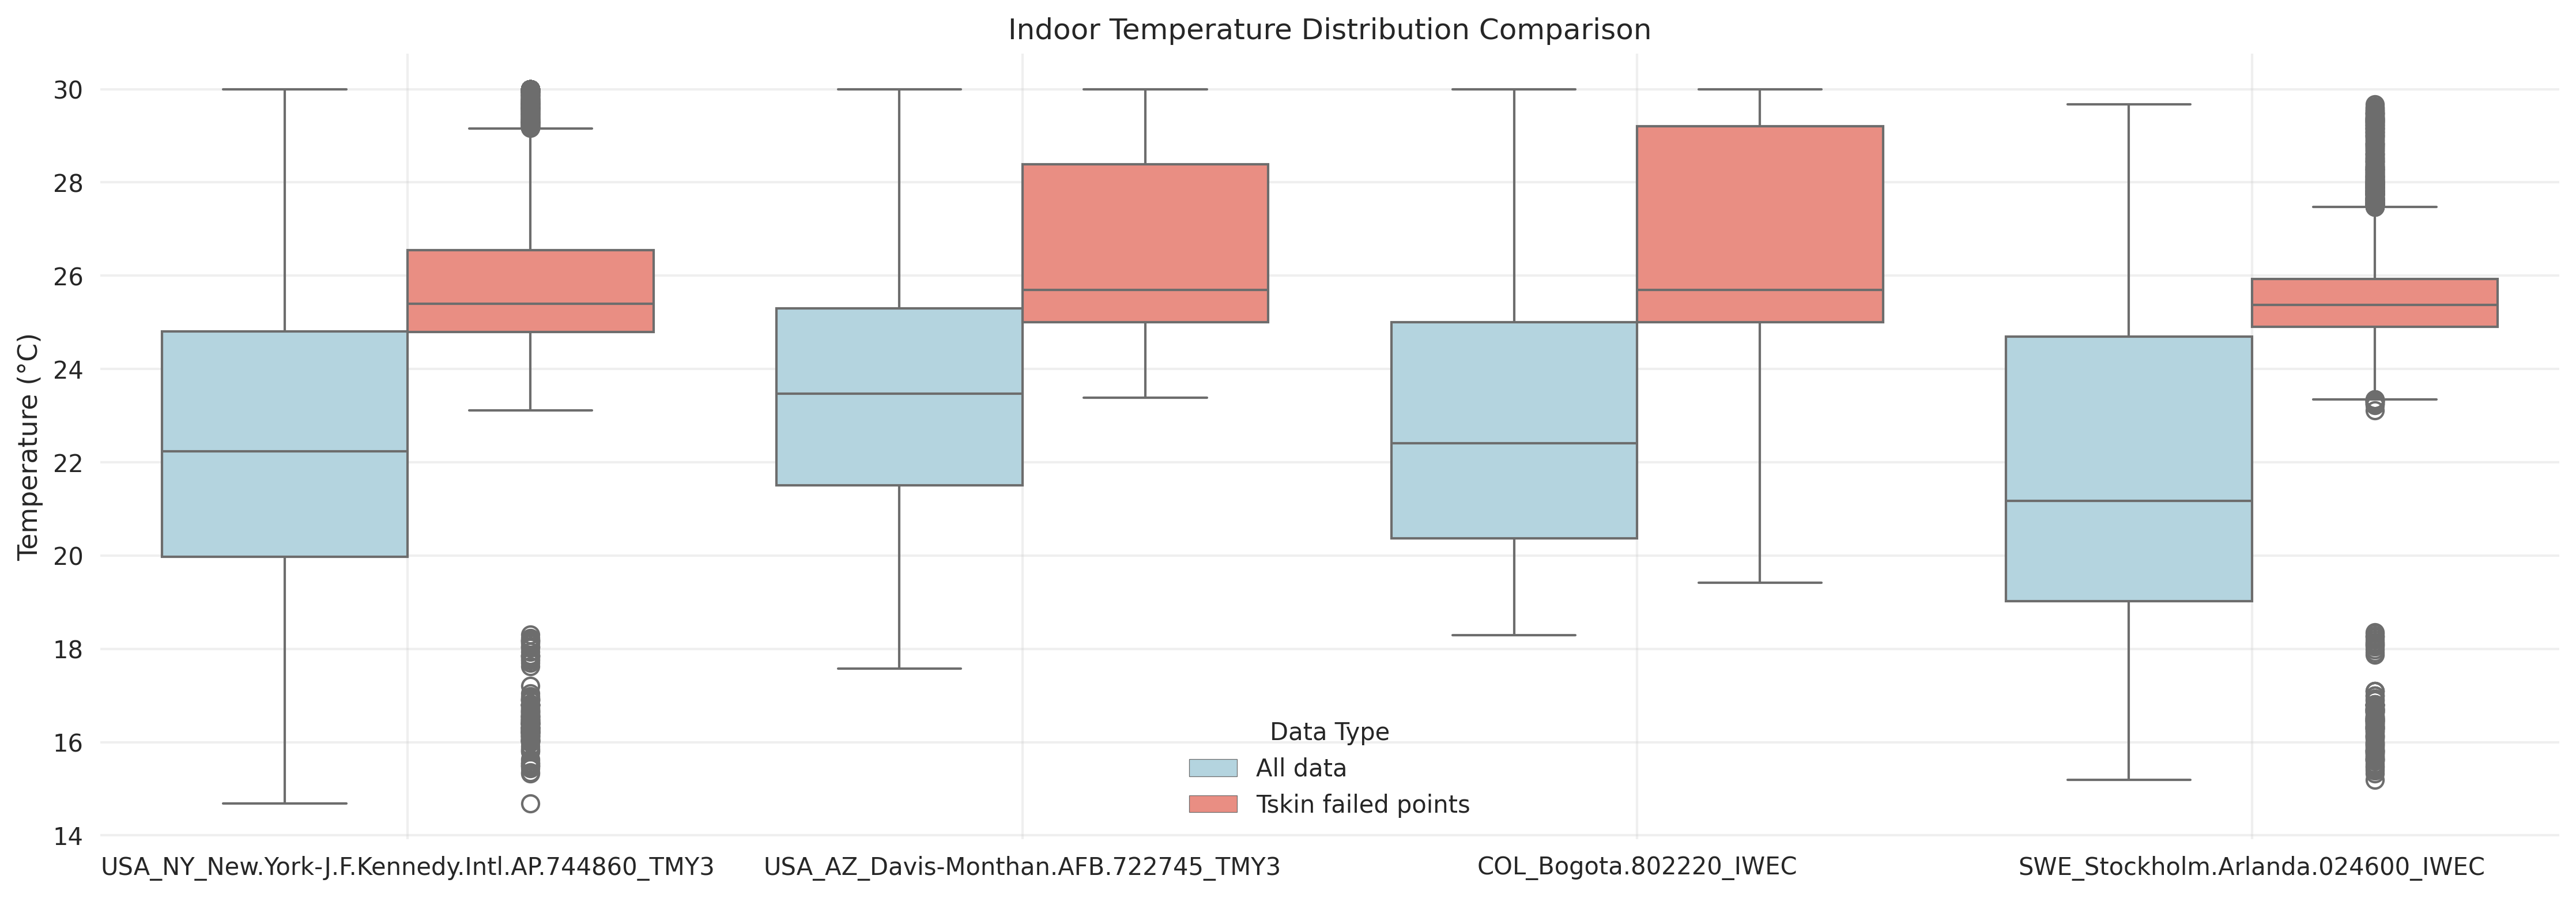
\includegraphics[width=0.75\linewidth]{figs/temp_distribution_comparison.png}
    \caption{Comparison of the air temperature distribution across all data points and the subset of instances where the $T_{skin}$ condition was not met with \texttt{pv-tsk-strict} mode}
    \label{fig:tsk_ta_distribution}
\end{figure}

Incorporating physiological metrics such as $T_{skin}$ into HVAC control logic significantly enhanced occupant comfort with minimal additional energy consumption. This result emphasizes the promising potential of physiology-informed control strategies to transform conventional building management approaches.



\subsection{Robustness Under Stochastic Weather Conditions}
The use of stochastic weather perturbations throughout our simulations provides inherent validation of our findings' statistical robustness. Despite random variations of $\pm$2.5$^\circ$C (1$\sigma$) applied to temperature readings at each 15-minute timestep—equivalent to sensor uncertainty and microclimate variations in real buildings—the performance hierarchy remains remarkably stable:
\begin{itemize}
    \item Grid-search optimized variants (pmv-o, lightgbm-o, pv-o) consistently rank in the top three positions across all climates
    \item Energy savings percentages show low variance: optimized PMV achieves 15-18.5\% savings with less than $\pm$2\% variation across weather realizations
    \item Comfort metrics remain stable: median PMV stays within $\pm$0.1 of target despite weather perturbations
\end{itemize}

This stability under stochastic conditions demonstrates that our findings are not artifacts of specific weather patterns but represent fundamental differences in control strategy effectiveness. The consistent performance gaps between optimized and naive controllers across thousands of unique weather realizations provide strong statistical evidence for our conclusions without requiring extensive Monte Carlo studies.
\section{Limitations and Future Work}

\subsection{Limitations}

\paragraph{Scope of Physiological Modeling:} The current implementation relies on Gagge’s two-node model to constrain physiological variables (core and skin temperature, skin wettedness). While widely used, this model simplifies thermal regulation and may not fully capture inter-individual variability or responses under extreme thermal conditions, physical exertion, or transient exposures.

\paragraph{Soft Constraints and Lack of Hard Guarantees:} The physiological constraints are enforced via soft penalties, which guide but do not guarantee adherence to biophysical bounds. In rare cases, especially under high imputation uncertainty or data sparsity, the model may still yield borderline physiological outputs that would not be biologically plausible under strict energy balance.

\paragraph{Dataset Bias and Underrepresented Populations:} Despite combining two large-scale datasets, certain groups—such as older adults, children, or individuals in tropical and arid climates—remain underrepresented. As a result, predictions for these populations may not generalize without additional targeted data.

\paragraph{Reliance on MAR Assumption:} While statistical tests and data context support the Missing At Random (MAR) assumption, any unobserved dependencies influencing missingness (i.e., potential MNAR characteristics) could theoretically affect imputation accuracy. However, VAE-based methods are generally considered robust under MAR, which we established as the most plausible scenario.

\paragraph{Operational Feasibility for Real-Time Applications:} While model interpretability and prediction quality are improved, the added complexity of latent-variable inference and physiology-based losses increases training and inference time. This may limit near-term deployment in embedded or low-latency building control systems without further optimization.


\subsection{Future Work}
\noindent We therefore believe there are at least the following possible directions of future work for PINN-VAE and its variants for thermal sensation:
\paragraph{Joint Optimization of Comfort and Physiology:} Given that PINN-VAE outputs not only thermal sensation but also skin and core temperatures, future work could explore control algorithms that co-optimize predicted thermal comfort and physiological deviation from neutral. This opens new opportunities for occupant-aware HVAC strategies that balance subjective sensation with biophysical safety margins.

\paragraph{Integration of Wearable and Streaming Data:} Future deployments may leverage wearable sensors or IoT devices to dynamically update personal physiological inputs (e.g., real-time skin temperature or heart rate), enabling the PPI interface to adapt to intra-occupant variation or temporal changes such as illness, stress, or activity level.

\paragraph{Architectural Simplification and Model Compression:} To support deployment in building systems with limited computational capacity, model compression techniques such as pruning, quantization, or teacher-student distillation could be applied to PINN-VAE. These techniques would aim to preserve interpretability while reducing inference time and memory usage.

\paragraph{Alternative Physiological and Comfort Models:} The current architecture could be extended to accommodate other biothermal models (e.g., Stolwijk\cite{Stolwijk1971} or multi-segment models like JOS3\cite{Takahashi2002JOS}) or adaptive comfort formulations that better reflect behavioral and cultural variability. Comparative evaluation would help assess trade-offs in complexity and predictive value.

\paragraph{Field Validation in Operational Settings:} Beyond retrospective evaluation, a key next step is validating PINN-VAE in real-world building environments, comparing predictions to occupant feedback and observed control behavior. This will test not only accuracy but also acceptance and integration into control workflows.

\section{Conclusions}
This study introduced a physiology-informed neural framework (PINN-VAE) that jointly addresses two core challenges in thermal comfort modeling: (i) imputing missing values in large observational datasets and (ii) improving predictive performance while preserving physiological interpretability. By embedding soft physiological constraints into a variational autoencoder pipeline and leveraging both tabular and personal-profile inputs, our model successfully balances the flexibility of data-driven imputation with the structure of thermoregulatory realism.

We demonstrate that PINN-VAE achieves comparable or superior performance to traditional state-of-the-art models, particularly near the thermal neutral zone, where directional prediction errors are often most critical for occupant-centric applications. The inclusion of intermediate physiological outputs—core and skin temperatures—not only constrains unrealistic predictions but also offers interpretability advantages unavailable in tree-based or purely statistical models.

Furthermore, the availability of intermediate physiological outputs ($\hat{T}_{\text{core}}, \hat{T}_{\text{skin}}, \hat{w}$) offers enhanced interpretability; beyond predicting sensation, monitoring these variables could enable systems to infer underlying physiological states, potentially allowing for more proactive or health-aware environmental control strategies that anticipate discomfort or thermal stress.

Beyond thermal comfort, the PINN-VAE architecture offers a generalizable framework for combining latent-variable learning with physics-informed constraints. Its use could extend to domains such as biomechanics, energy metabolism modeling, or any setting where tabular physiological data are incomplete yet governed by known physical relationships.

The Personalized Physiology Interface (PPI) further strengthens this framework by enabling the use of raw demographic variables (e.g., age, height, gender, weight) without degrading predictive performance. In doing so, the model preserves important physiological signal diversity without needing population-wide feature averaging or scaling.

Compared to baseline LightGBM and unconstrained VAE architectures, our framework shows a measurable reduction in neutral-zone RMSE and direction-penalty asymmetry, reinforcing the hypothesis that physiology-informed modeling improves both accuracy and robustness. Overall, PINN-VAE offers a promising and interpretable path forward for occupant-aware control, particularly in systems where physiological realism and explainability are essential for deployment.



\section*{Data and Code Availability}
The code developed for the PINN-VAE model and the analysis presented in this paper is available on GitHub at [URL Currently Private] The final imputed dataset, generated using the best-performing model fold as described in Section~\ref{sec:PINN_VAE_Arch}, is available at request (currently sitting on private repository on github). The original ASHRAE Global Thermal Comfort Database II and Chinese Thermal Comfort Datasets are publicly available from their respective sources cited in the text.
\section{Conclusions}
This study presents the first comprehensive co-simulation framework directly integrating data-driven thermal sensation models with EnergyPlus, overcoming historical reliance on PMV as a proxy for occupant comfort. By leveraging a dataset of 148,148 thermal sensation votes from the ASHRAE Global Thermal Comfort Database II and Chinese datasets, we enabled real-time predictions of occupant thermal sensation during building simulation—a capability previously challenging to achieve.

Our evaluation of seven control strategies across four diverse climate zones yielded several critical insights. First, optimized PMV-based control via grid-search algorithm significantly outperformed naive comfort-driven control, achieving 15–18.5\% energy savings compared to a 4.3–23.5\% energy penalty with non-optimized PMV control. Remarkably, optimized PMV achieved comparable energy efficiency to advanced machine learning models (LightGBM and PINN-VAE) while requiring substantially lower computational resources. Among ML models, LightGBM exhibited robust predictive performance but at tenfold runtime relative to optimized PMV. Meanwhile, the PINN-VAE model, although novel in incorporating physiological realism through predictions of skin temperatures ($T_{skin}$), showed only marginal improvements in energy performance while requiring prohibitively long runtimes (10–15 minutes per year simulation), potentially limiting its direct real-time applicability.

The ability of PINN-VAE to predict physiological variables nonetheless introduced valuable opportunities for enhancing occupant comfort. By explicitly incorporating predicted skin temperature into HVAC control logic, we achieved a notable 14.85\% improvement in comfort hours at a modest 1.97\% energy increase, demonstrating the practical potential of physiologically-informed control strategies. The incorporation of stochastic weather perturbations in all simulations ensures these results reflect expected performance under real-world weather variability, not idealized conditions.

It's also important to point out our co-simulation methodology revealed that naive ML-based controllers frequently could encounter actuator saturation—a critical deployment challenge invisible to traditional comfort prediction studies—thereby validating the necessity of integrated simulation frameworks for practical control development.

Critically, our re-analysis showed that naive LightGBM and PV controllers appeared to outperform PMV only because they were frequently clipped to 12$^\circ$C or 30$^\circ$C (actuator saturation), not because they improved comfort.
This finding underscores that any future ML-based control strategy must explicitly account for actuator bounds when optimizing setpoints; otherwise, apparent energy savings may simply reflect saturation at the extremes.

The core implication of our findings explicitly challenges the assumption that increasing model complexity inherently yields superior HVAC performance. Instead, carefully optimized classical models such as PMV provide near-equivalent energy and comfort performance at significantly reduced computational and infrastructural costs, thus offering a highly practical pathway for broad deployment. The demonstrated feasibility and performance of our co-simulation framework underscore that future research should prioritize addressing critical operational constraints—such as continuous setpoint adjustments, multi-zone coordination, and adaptive predictive horizons—rather than solely refining comfort prediction accuracy.

For the building controls community, this study reinforces that integrated, occupant-centric co-simulation frameworks are both viable and valuable. By shifting research and development efforts towards practical optimization strategies and advanced physiological sensing integration, we can significantly enhance HVAC operational efficacy. Future work should extend this co-simulation methodology across additional building types, HVAC systems, and occupant demographics, ensuring broader generalizability and practical relevance. Ultimately, addressing fundamental physical and operational constraints is crucial for fully realizing the potential benefits of advanced comfort models in real-world building control applications.

\newpage
\section*{Nomenclature}
\begin{table}[h!]
\centering
\resizebox{\textwidth}{!}{
\begin{tabular}{ll}
\toprule
\textbf{Symbol / Acronym} & \textbf{Description} \\
\midrule
\textbf{PMV}          & Predicted Mean Vote – analytical thermal sensation index (ISO 7730) \\
\textbf{TSV}          & Thermal Sensation Vote – occupant-reported thermal comfort level \\
\textbf{PINN-VAE}     & Physics-Informed Neural Network with Variational Autoencoder \\
\textbf{LightGBM}     & Light Gradient Boosting Machine – tree-based ML model for tabular data \\
\textbf{EUI}          & Energy Use Intensity – building energy consumption per unit floor area (kWh/$m^2$) \\
$T_{skin}$            & Mean skin temperature ($^\circ$C) – predicted or modeled via biophysical models \\
$T_{core}$            & Core body temperature ($^\circ$C) – estimated using Gagge's two-node model \\
\textbf{clo}          & Clothing insulation level (1 clo $\approx$ 0.155 $m^2$·K/W) \\
\textbf{met}          & Metabolic rate (1 met $\approx$ 58.2 W/$m^2$) \\
\textbf{HVAC}         & Heating, Ventilation, and Air Conditioning system \\
\textbf{ASHRAE}       & American Society of Heating, Refrigerating and Air-Conditioning Engineers \\
\textbf{ISO 7730}     & International Standard defining PMV/PPD indices \\
\textbf{DOE}          & U.S. Department of Energy – defines standard climates/building archetypes \\
\textbf{Sinergym}     & Python–EnergyPlus co-simulation and RL environment \\
\textbf{EnergyPlus}   & Whole-building energy simulation engine \\
\textbf{EMS}          & Energy Management System – rule-based control scripting in EnergyPlus \\
\textbf{PV-o}         & PINN-VAE optimized control mode \\
\textbf{PMV-o}        & PMV control mode optimized via grid-search \\
\textbf{LB-o}         & LightGBM control mode optimized via grid-search \\
\textbf{RBC}          & Rule-Based Controller – baseline on/off control scheme \\
\textbf{Comfort hours} & Simulation hours where TSV is within comfort range ($-0.5 \leq$ TSV $\leq +0.5$) \\
\textbf{Runtime}      & Time to execute one year of simulation (seconds) \\
\bottomrule
\end{tabular}
}
\caption{List of symbols and acronyms used throughout the paper.}
\end{table}



% %% The Appendices part is started with the command \appendix;
% %% appendix sections are then done as normal sections
% \appendix
% \section{Example Appendix Section}
% \label{app1}

% Appendix text.


\bibliographystyle{elsarticle-num}
\bibliography{cas-refs}

\end{document}

\endinput
%%
%% End of file `elsarticle-template-num.tex'.
